%%
%% This is file `thesis-ex.tex',
%% generated with the docstrip utility.
%%
%% The original source files were:
%%
%% uiucthesis2014.dtx  (with options: `example')
%% 
\def\fileversion{v2.25b} \def\filedate{2017/05/02}
%% Package and Class "uiucthesis2014" for use with LaTeX2e.
\documentclass[12pt,edeposit,fullpage]{uiucthesis2014}

% references at the end of each chapter
\usepackage[round,sectionbib]{natbib}
\usepackage{chapterbib}

\usepackage{amsmath}
\usepackage{amssymb}
\usepackage{bibentry}
\usepackage{graphicx}
\usepackage{hyperref}
\usepackage{caption}
\usepackage{subcaption}
\usepackage{rotating}
\usepackage{listings}
\usepackage{fancyvrb}

\usepackage{lscape}
\usepackage{longtable}


\usepackage{adjustbox}


\usepackage[ruled,vlined,linesnumbered]{algorithm2e}

\usepackage{listings} % code in snippets
\usepackage{color} % color syntax

\definecolor{mygreen}{rgb}{0,0.6,0}
\definecolor{mygray}{rgb}{0.5,0.5,0.5}
\definecolor{mymauve}{rgb}{0.58,0,0.82}
\usepackage[T1]{fontenc}


\usepackage[titletoc]{appendix}

\lstset{ %
  backgroundcolor=\color{white},   % choose the background color
  basicstyle=\footnotesize,        % size of fonts used for the code
 frame=single,	   
  breaklines=true,                 % automatic line breaking only at whitespace
    numbers=left,                    % where to put the line-numbers; possible values are (none, left, right)
  numbersep=5pt,
  numberstyle=\color{mygray},
  captionpos=b,                    % sets the caption-position to bottom
  commentstyle=\color{mygreen},    % comment style
  escapeinside={\%*}{*)},          % if you want to add LaTeX within your code
  keywordstyle=\color{blue},       % keyword style
  stringstyle=\color{mymauve},     % string literal style
    showspaces=false,
  showstringspaces=false,
  upquote=true,
}
%  literate={``}{\textquotedblleft}1,  %set right quote mark
 % deletestring=[b]",  % del left quote mark
  
\usepackage{multirow}
\usepackage[normalem]{ulem}
\useunder{\uline}{\ul}{}

% First level headings in table of contents
\setcounter{tocdepth}{1}


\def\aap{{A\&A}}
\def\AaA{{A\&A}}
\def\AJ{{AJ}}
\def\aj{{AJ}}
\def\ApJ{{ApJ}}
\def\apj{{ApJ}}
\def\apjl{{ApJL}}
\def\ApJL{{ApJL}}
\def\ApJSupp{{ApJS}}
\def\MN{{MNRAS}}
\def\mnras{{MNRAS}}
\def\mnrasl{{MNRAS Letters}}
\def\pasp{{PASP}}
\def\jcap{JCAP}
\def\pasj{{PASJ}}
\def\nat{Nature}
\def\ARAA{{ARA\&A}}
\def\apjs{{ApJS}}
\def\araa{{ARA\&A}}
\def\apss{{Ap\&SS}}
\def\cjaa{{ChJAA}}
\def\aaps{{A\&AS}}

\newcommand{\eg}{{e.g., }}
\newcommand{\ie}{{i.e., }}
\newcommand\blfootnote[1]{%
  \begingroup
  \renewcommand\thefootnote{}\footnote{#1}%
  \addtocounter{footnote}{-1}%
  \endgroup
}

%Define Robert Comment

\newcommand\RC[1]{\color{red}{\textbf{ Robert Comment: }{#1} }\color{black}}

% put figure on a new page
\renewcommand{\floatpagefraction}{0.1}

\newsavebox{\FVerbBox}
\newenvironment{FVerbatim}
 {\VerbatimEnvironment
  \begin{center}
  \begin{lrbox}{\FVerbBox}
  \begin{BVerbatim}}
 {\end{BVerbatim}
  \end{lrbox}
  \fbox{\usebox{\FVerbBox}}
  \end{center}}



\makeatletter
\newenvironment{breakablealgorithm}
  {% \begin{breakablealgorithm}
   \begin{center}
     \refstepcounter{algorithm}% New algorithm
     \hrule height.8pt depth0pt \kern2pt% \@fs@pre for \@fs@ruled
     \renewcommand{\caption}[2][\relax]{% Make a new \caption
       {\raggedright\textbf{\ALG@name~\thealgorithm} ##2\par}%
       \ifx\relax##1\relax % #1 is \relax
         \addcontentsline{loa}{algorithm}{\protect\numberline{\thealgorithm}##2}%
       \else % #1 is not \relax
         \addcontentsline{loa}{algorithm}{\protect\numberline{\thealgorithm}##1}%
       \fi
       \kern2pt\hrule\kern2pt
     }
  }{% \end{breakablealgorithm}
     \kern2pt\hrule\relax% \@fs@post for \@fs@ruled
   \end{center}
  }
\makeatother

\nocopyrightpage

\begin{document}

\title{Machine Learning and Information-Theoretic Approaches for Financial Applications}
\author{Kelechi Moise Ikegwu}
\department{Informatics}
\phdthesis
\advisor{Robert J.\ Brunner}
\degreeyear{2021}
\committee{
    Professor Robert J.\ Brunner,  Chair,  Director of Research\\
    Professor Theodore Sougiannis\\
    Assistant Professor Jeff McMullin\\
    Assistant Professor Joseph Yun}
\maketitle

\frontmatter

%% Create an abstract that can also be used for the ProQuest abstract.
%% Note that ProQuest truncates their abstracts at 350 words.
\begin{abstract}

Firm-specific information contributes to resource allocation in capital markets.  The prediction and inference of future firm-specific information are often critical factors for a prosperous economy.  Machine Learning and Information Theory offer alternative methods to aid in the prediction and inference of future firm-specific information.  Thus we explore approaches from machine learning and information theory to improve existing research areas in finance.  

%Maybe Remove SML?
In Chapter \ref{Chapter:SML} we introduce an agnostic framework called SML that integrates a query-like language to simplify the development of machine learning pipelines.  We show that SML significantly reduces the code one has to write to develop parts of a machine learning pipeline. In Chapter \ref{Chapter:ABIS} we utilized random forest trees to predict the annual direction of profitability for firms with a minimal amount of information.  We demonstrate that we can out-perform benchmark models typically used in financial accounting research settings.  

Major public firms announce their annual earnings during the first quarter of the year.  The embedding information in these announcements effects the announcing firm and is transferred or incorporated in other firms.  Existing literature in finance and accounting focuses on measuring information transfers as effects stemming from firm-specific information releases.  In Chapter \ref{Chapter:PyIF} we discuss a solution to estimate information transfer via transfer entropy between random processes.  We show that our solution to estimate information transfer scales better than and is up to 1,072 times faster than all open source existing solutions for large datasets.  In Chapter \ref{Chapter:EATE} we present an alternative approach to estimate information transfer between firms centered around earnings announcements.  We show that information transfer between firms is stronger for firms on days with unexpected earnings news.  We also show that communities of firms are not adequately captured by characteristics that are the focus of existing literature.

\end{abstract}

%% Create a dedication in italics with no heading, centered vertically
%% on the page.
\begin{dedication}
To my Father,  Mother,  Joshua,  Sandra,  Ezinne,  Natalia,  Khamille,  and Khalil.
\end{dedication}

%% Create an Acknowledgements page, many departments require you to
%% include funding support in this.
\chapter*{Acknowledgments}

First and foremost, I would like to thank my advisor,  Robert Brunner, for his guidance,  patience,  and support during my graduate studies at the University of Illinois at Urbana-Champaign.
I also wish to thank my committee members, Theodore Sougiannis, Jeff McMullin, and Joseph Yun,  for their help and support.
I am also grateful to Junhyung Kim, Vincent Reverdy, William Biscarri,  Samantha Thrush,  Matias Carrasco Kind,  Jacob Trauger,  Alice Perng, and Howard Hardiman.

\begin{flushright}
--- Kelechi Moise Ikegwu
\end{flushright}

\vspace{10mm}

This work was partially funded by the Graduate College Fellowship program at the University of Illinois.  The work was partially funded by the National GEM Consortium.  This work utilizes resources provided by the Innovative Systems Laboratory at the National Center for Supercomputing Applications at the University of Illinois at Urbana-Champaign.

%% The thesis format requires the Table of Contents to come
%% before any other major sections, all of these sections after
%% the Table of Contents must be listed therein (i.e., use \chapter,
%% not \chapter*).  Common sections to have between the Table of
%% Contents and the main text are:
%%
%% List of Tables
%% List of Figures
%% List Symbols and/or Abbreviations
%% etc.

\tableofcontents
%\listoftables
%\listoffigures


    

%% Create a List of Abbreviations. The left column
%% is 1 inch wide and left-justified
%\chapter{List of Abbreviations}
%
%\begin{symbollist*}
%\item[CA] Caffeine Addict.
%\item[CD] Coffee Drinker.
%\end{symbollist*}

%% Create a List of Symbols. The left column
%% is 0.7 inch wide and centered
%\chapter{List of Symbols}
%
%\begin{symbollist}[0.7in]
%\item[$\tau$] Time taken to drink one cup of coffee.
%\item[$\mu$g] Micrograms (of caffeine, generally).
%\end{symbollist}

\mainmatter

\chapter{Introduction}


The economic goal of a society is to maximize wealth by allocating resources efficiently. Capital markets (such as the stock market) provide a method to help allocate resources efficiently. The prediction and inference of future financial events are often critical to achieve the economic goal. Firm specific information contribute to how resources (i.e labor, capital, and natural resources) are allocated in capital markets. The prediction of a future state for a firm (such as the firm's profitability, financial condition, or revenue growth) is an important factor to contribute to how resources should be allocated.  There are many methods used to predict or inform about the future state of a firm.  


\section{Machine Learning}

Machine Learning encompasses a vast set of statistical tools for understanding data and making predictions and inference. These tools fall into supervised or unsupervised categories. For data-driven problems typically we have a response variable (or labels)  referred to as \(Y\) and \(p\) independent variables (or features) refereed to as \(X\). If an assumption is made that there is some relationship between \(Y\) and \(X\) the relationship can be expressed as:

\begin{equation}
\label{eq:function}
Y = f(X) + \epsilon
\end{equation}

\noindent In eq. \ref{eq:function} \(f\) is an unknown function that models the relationship between \(X\) and \(Y\) with  \( \epsilon \) noise.  In most cases it is not possible to perfectly model \(f\) with real-world data and \(f\) is estimated (\(\hat{f}\)). In eq.\ref{eq:function} if \(Y\) is a quantitative variable then regression techniques are used estimate \(f\), however if \(Y\) is a qualitative variable then classification techniques are used.   \(\hat{f}\) is sought for inference where one wants to estimate \(f\) to understand how \(\hat{Y}\) (predicted labels) changes as one adjusts features. \(\hat{f}\) is also sought for prediction where the only concern is the accuracy of predictions for \(Y\). Machine learning provides a variety of approaches to estimate \(f\) for prediction and inference (see \cite{ISL:C1}).

Machine learning problems typically fall into either supervised learning, semi-supervised learning, or unsupervised learning. With supervised learning one wants to fit a model on labels using a set of features. Semi-supervised learning consists of an environment with features and some corresponding labels. Typically in this setting one wishes to use the given features and partial labels to determine what the remaining missing labels are. Lastly with unsupervised learning one has features and no associated labels and seeks to find structure between the features. Currently, the research in this book will only utilize supervised learning. 

\subsection{Supervised Learning} \label{sec:SupervisedLearning}
In a supervised learning paradigm it is not enough to only have \(\hat{f}\) estimate \(f\) well on a dataset. \(\hat{f}\) is often sought to learn a dataset well enough to generalize well to new data that  \(\hat{f}\) has never seen before. To achieve this goal, a common methodology is to partition the data into a training set and testing set. The training set is used to train the model. The testing data is only used to assess the \(\hat{f}\)'s ability to generalize well to new data. The ratio of data used to train and assess the model is typically determined by the practitioner.  A specific \footnote{There are many error metrics that can be used however, for the sake of brevity MSE is the only error metric that will be discussed. } way to estimate \(\hat{f}\)'s performance is use  an error metric such as mean squared error (MSE) given by  

\begin{equation}
\label{eq:MSE}
MSE = \frac{1}{n} \sum_{i=1}^n (y_i -\hat{f}(x_i))^2
\end{equation}

\noindent In eq. \ref{eq:MSE} \(y_i\) and \(x_i\) are the \(i^{th}\) observations of the labels and features respectively. \(\hat{f}(x_i)\) is the prediction of \(\hat{f}\) for the \(i^{th}\) observation and \(y_i\) is the label for the \(i^{th}\) observations. There will be a training MSE indicating the mean error of \(\hat{f}\) learning the training data. Subsequently there is a testing MSE associated with mean error of \(\hat{f}\) on the withheld testing data. A model with a very small testing MSE generalizes well to the withheld data. Often, the training MSE and testing MSE differ where the training MSE  underestimates the MSE for the test MSE \cite{ISL:Chapter5}. To combat this issue there are many approaches that can produce a more accurate MSE of how \(\hat{f}\) will generalize to new data.

\subsection{Validation Approaches} \label{sec:validationApproach}

An alternative approach to training and assessing \(\hat{f}\) on training and testing sets respectively is to create a validation dataset by randomly sampling the training dataset. The sampling method is determined by the researcher/practitioner. \(\hat{f}\) is then trained on the training data and the trained model is assessed with validation data. The validation MSE is more indicative of the test MSE. However there are issues with this approach. For example the validation data-set is comprised of randomly sampled data. Given the random data the validation MSE highly variable. To combat this issue cross-validation can be used to  decrease the variability of the validation MSE.

A common cross-validation technique is \(k\)-fold cross-validation where the training data is split into \(k\) separate folds (see Figure \ref{fig:KFoldValidation}). The first fold is withheld and used as the validation data-set to assess the model's performance. The remaining \(k-1\) folds are used to train the model. For the next iteration the same procedure is followed where the 2nd fold is withheld to serve as the validation data-set to assess the model (see Figure \ref{fig:KFoldValidationExplain}) and the other \(k-1\) folds are used. This process repeats \(k\) times and  produces \(k\) \(MSE\) scores (\(MSE_1, MSE_2, ... , MSE_k\)). The \(k\)-fold CV estimate is  computed by averaging the MSE fold values

\begin{equation}
\label{eq:CV}
CV = \frac{1}{k} \sum_{i=1}^k MSE_i
\end{equation}

\noindent where \(k\) is the number of folds. 

Selecting a large value \(k\) can be computationally expensive as the model must be retrained on \(k\) separate folds. In addition to this, the selection of \(k\) can effect the model's ability to generalize to new data well. Typically with a smaller value of \(k\) you have more bias and a larger value of \(k\) has more variance. For example consider when \(k=3\) and \(k=10\), the training folds will have \(n_{train}\) observations where  \( n_{train}= \frac{(k-1)n}{k}\) and the validation fold will have \(n_{validation}\) observations where \( n_{validation}= \frac{k-(k-1)n}{k}\). When \(k=10\), 90\% of the data is used to train the model and the remaining 10\% is used to assess the model. The model is trained on very similar datasets and the predictions from the model on the cross-validation datasets are highly correlated. This results in a model with high variance. If \(k=3\) 66.7\% of the data is used to train the model and the remaining 33.3\% of the data is used to assess the model. CV averages fewer predictions that are less correlated with each other, since the overlap between the training sets are smaller.  This results in a CV score with lower variance and higher bias. 

% wrap ML up.

\section{Network Science} \label{sec:NetworkScience}

% context to how network science is used in Finanical Markets

A network (or graph) consists of a collection of nodes joined by connections between the nodes (commonly referred to as edges). Networks can be formed from data to offer a representation of the structure of data which subsequently allows many analysis techniques to be performed. Network Theory involves the study of networks as a representation of relationships between nodes. Throughout this section a network will be denoted by \(G\), the number of edges in a network will be denoted by \(m\), and the number of nodes will be denoted by \(n\).  A graph with \(n\) nodes and \(m\) edges is denoted as \(G(n,m)\).

Graphs do not have to specify the direction of an edge. Graphs with this property are referred to as a undirected graph. For example if Node \(A\) and Node \(B\) are connected a undirected graph will not distinguish whether Node ``A" is connected to Node ``B" or vice-versa;  an undirected graph will only retain information about nodes \(A\) and \(B\) having a connection. Figure \ref{fig:ExampleNetwork} shows an example of a undirected graph \(G(7,16)\). The amount of edges a particular node has is referred to as the degree of the node. In Figure \ref{fig:ExampleNetwork}, the node ``FB" has a degree of 6 because it is connected to 6 other nodes.
Degree is a common metric used in network theory.

It is also possible for a graph to retain additional information about edges. Another source of information are the direction of the edges; graphs that store information about the directions of edges are called directed graphs. For example if Node ``A"  is connected to Node ``B" a directed graph would contain information that Node ``A"  has an edge to Node ``B" but Node ``B" does not have an edge to Node ``A". Figure \ref{fig:ExampleNetworkDirected} shows an example of a directed graph; in Figure \ref{fig:ExampleNetworkDirected} there is an edge from ```JNJ" to ``FB"  however there is no edge from ``FB" to ``JNJ".

Another source of information that graphs can retain are edge weights and are called weighted networks (or weighted graphs). Instead of having a binary connection to determine whether an edge is present or not it can be useful to measure the strength between connections of nodes.For example if you can have an attribute to determine the strength between nodes such as TE estimates, TE estimates can be used as the weight value of an edge to determine the strength of information flow between nodes. Edge weights are applicable to both directed and undirected graphs ergo it is possible to have a undirected weighted graph or directed weighted graph. Figure \ref{fig:ExampleNetworkDirectedWeighted} contains an example of a directed weighted network. 

Under certain circumstances it is more convenient to express a graph as an adjacency matrix.  For example consider the graph in Figure \ref{fig:ExampleNetwork}, if this were expressed as a table with column and row headers Table \ref{tab:ExampleTable} would be produced. 

However it is mathematically more convenient to express Table \ref{tab:ExampleTable} as an adjacency matrix (see Eq \ref{eq:adjacencyMatrix}).

\begin{gather}
A =
 \begin{bmatrix}
    0 & 1 & 1 & 1 & 0 & 1 & 1 \\
    1 & 0 & 1 & 1 & 0 & 1 & 1 \\
    1 & 1 & 0 & 1 & 1 & 0 & 0 \\
    1 & 1 & 1 & 0 & 1 & 1 & 1 \\
    0 & 0 & 1 & 1 & 0 & 0 & 0 \\ 
    1 & 1 & 0 & 1 & 0 & 0 & 1 \\
    1 & 1 & 0 & 1 & 0 & 1 & 0 \\
  \end{bmatrix}
  \label{eq:adjacencyMatrix}
\end{gather}

\noindent Similar to Table \ref{tab:ExampleTable} each matrix element (\(A_{ij}\)) in \(A\) is assigned a 1 or 0 based on if there is a connection between a row index (\(i\))  and column index \(j\). You'll notice in Eq \ref{eq:adjacencyMatrix} that the matrix is symmetric because 
the direction of edges are not taken into account; ergo if node \(i\) and node \(j\) are connected \(A_{ij}\) and \(A_{ji}\) have a value of 1. It is also possible to represent directed graphs by assigning a 1 to a matrix element \(A_{ij}\) where node \(i\) is connected to node \(j\). Lastly you can express the weight of edges in adjacency matrices by assigning non-binary values to matrix elements.

\subsection{Analysis of Networks}
After forming a network from data, common metrics are often sought to help describe the structure of the network.  The first metric are the degree of nodes where the degree  can be defined in Eq \ref{eq:degree} as the sum of edges for a particular node. In Figure \ref{fig:ExampleNetworkDegree} the node sizes are scaled based on the degree .

\begin{equation}
    \label{eq:degree}
    k_i =  \sum_{j=1}^{n}A_{ij}
\end{equation}

\noindent where \(A\) is an adjacency matrix. Subsequently you can have degrees for directed networks such as in-degree which counts the amount of edges that are connected to node \(i\) (see Eq \ref{eq:indegree}). Whereas out-degree counts the amount of edges that node \(i\) is connected to (see Eq \ref{eq:outdegree}).

\begin{equation}
    \label{eq:indegree}
    k_i^{in} =  \sum_{j=1}^{n}A_{ij}
\end{equation}

\begin{equation}
    \label{eq:outdegree}
    k_i^{out} =  \sum_{i=1}^{n}A_{ij}
\end{equation}

\noindent The density of the network provides a numerical value for the portion of potential connections in a network that are actually connected. If all potential connections in a network are present then the density will have a numerical value of 1 and if there are no connections in an undirected network the density will be 0. The maximum number of potential connections in a network is \(n(n-1)/2\).  The degree summed for all nodes is \(m\) (for directed networks the summed in-degree and out-degree for all nodes is \(m\)). The density for a graph can be defined as:

\begin{equation}
    \label{eq:density}
    D_u = \frac{2m}{n (n-1)}
\end{equation}

Centrality is another metric often sought to measure the importance of nodes in networks. Measuring the degree of nodes in relation to other nodes is called degree centrality (see Eq \ref{eq:degreeCentrality}). 

\begin{equation}
    \label{eq:degreeCentrality}
    C_i^d =  k_i = \sum_{i=1}^{n}A_{ij}
\end{equation}



\section{Information Transfer in Financial Markets} \label{IFinFM}
% Tailor this section such that I dicuss Information Transfer in  a traditional context first, then explain transfer entropy.
The price discovery process is important to achieve the economic goal of a society. Information is embedded in price and in an efficient market changes rapidly (if not instantaneously) when new information arrives. In particular how information transfers from one price to another is useful in the price discovery process. For example Apple Inc. announced that their new line of computers (Macs) would use central processing units (CPUs) developed in house and transition away from Intel) CPUs. In ideal settings this information will be reflected in Apple's stock price and Intel's stock price.

In the example above it is probable that additional information can be reflected in Intel's price change at a given moment. However, it is difficult to determine price changes for specific events. The entire set of  information that is reflected in the price change at a given time period is unknown.  Prior studies have examined the price changes over long windows such as days or weeks (see \cite{Foster1981} and \cite{Baginiski 1987}) or shorter windows such as days. These methodologies may have missed much of the price change process given the assumption that information effects the price within seconds.  Given the theory that markets are efficient and reflect information into price within seconds after the information is known, we seek suitable methods to measure information flow in financial markets.

\subsection{Information Theory } \label{sec:InformationTheory}
Information theory provides a framework for studying the quantification, storage, and communication of information \cite{InfoTheoryApplications}.  Information theory has the potential to be useful in the price discovery process given that it can offer alternative approach for understanding information in price. In particular it offers alternative methods to understand information transfer between dynamic processes (such as stock prices). In this dissertation, I measure information flow in financial markets with the relatively new measure transfer entropy (see \ref{} and \ref{}). Transfer Entropy (TE) quantifies the reduction in uncertainty in one random process from knowing past realizations of another random process (see \ref{}). For example it is unlikely to predict Intel's closing price tomorrow. However knowing Intel's price today reduces the amount of uncertainty in the prediction for it's price tomorrow. In addition to this, knowing Apple's price today may help further reduce the uncertainty in the future prediction. If Apple's price today helps to further reduce the uncertainty then TE will be positive indicating an information transfer from Apple to Intel. 

In 2000, Schreiber \cite{IntroToTransferEntropy} discovered TE and coined the name ``transfer entropy," although Milian Palus \cite{IntroToTransferEntropy2} also independently discovered the concept as well. To define TE, one must begin with the building blocks of information theory \footnote{For simplicity discrete events are used to introduce these concepts.}.  Shannon Information is defined as: 

\begin{equation}
\label{{eq:shannonInfo}}
h(x) = \log_2 \frac{1}{p(x)}
\end{equation}

\noindent where \(x\) is an event and \(p(x)\) is probability of \(x\) occurring. This definition implies that values of x with small probabilities contain more information. Consequently values of x that are more probable (or common) contain less information. Entropy is the amount of uncertainty or disorder in a random process.

\begin{equation}
\label{eq:Entropy}
H(X) =  \frac{1}{n} \sum_{i=1}^n  \log_2 p(x)
\end{equation}


\noindent Entropy is defined in eq. \ref{eq:Entropy} is the weighted average of shannon information.  Conditional entropy is the entropy after conditioning on another process (\(Y\)):

\begin{equation}
\label{eq:CondEntropy}
H(X|Y) = \sum_{y \in \Omega_y} p(y) H(X|y)
\end{equation}

\noindent In eq. \ref{eq:CondEntropy} \(y \in \Omega_y\) represents the occurrence of \(y\) in a set of possible events for \(y\) and \(H(X|y)\) represents conditional entropy on a single event \(y\) (or \(H(X|y) = \sum_{x \in \Omega_x}  \frac{p(x|y)}{\log_2p(x|y)} \)). Mutual Information quantifies the amount of information shared across random variables:

\begin{equation}
\label{eq:MutalInformation}
I(X,Y) = H(X) - H(X|Y) = H(Y) - H(Y|X)
\end{equation}

\noindent In eq. \ref{eq:MutalInformation} consider \(H(X) - H(X|Y)\),  \(H(X)\) computes the entropy of X and \(H(X|Y)\) computes the entropy of X conditioned on Y. The difference between \(H(X)\) and \(H(X|Y)\) captures the shared information between \(X\) and \(Y\). Mutual Information in a directed measure ergo \(I(X,Y) = I(Y,X)\).

Lagged mutual information \(I(X_t : Y_{t-k})\) can be used as a time-asymmetric measure of information transfer from \(Y\) to \(X\) where \(X\) and \(Y\) are both random processes, \(k\) is a lag period, and \(t\) is the current time period. However, lagged mutual information is unsatisfactory as it does not account for a shared history between the processes \(X\) and \(Y\) \cite{MIdiffTE}. While similar to lagged mutual information, transfer entropy (TE) also considers the dynamics of information and how these dynamics evolves in time \cite{IntroToTransferEntropy}. TE is also an asymmetric measure of information transfer. Ergo, TE computed from process \(A\) to process \(B\) may yield a different result than TE computed from \(B\) to \(A\). The information theoretic framework and these measures have led to a variety of applications in different research areas \cite{InfoTheoryApplications}, \cite{TEBook}.

TE considers the shared history between two processes via conditional mutual information. Specifically, TE conditions on the past of \(X_t\) to remove any redundant or shared information between \(X_t\) and its past. This also removes any information in the process \(Y\) about \(X\) at time \(t\) that is in the past of \(X\) \cite{b359}. Transfer entropy \(T\) (where the transfer of information occurs from \(Y\) to \(X\)) can be defined as:
\begin{equation}
T_{Y \rightarrow X} (t) \equiv I(X_t: Y_{t-k} |  X_{t-k})
\end{equation}

\noindent Kraskov \cite{kraskovEstimator} shows that transfer entropy can be expressed as the difference between two conditional mutual information computations: 

\begin{equation} 
T_{Y \rightarrow X}(t) = I(X_t | X_{t-k}, Y_{t-k}) -  I(X_t | X_{t-k}) 
 \end{equation} 

The intuition of this definition is that TE measures the amount of information in \(Y_{t-k}\) about \(X_t\) after  considering the information in \(X_{t-k}\) about \(X_t\). Put differently, TE quantifies the reduction in uncertainty about \(X_t\) from knowing \(Y_{t-k}\) after considering the reduction in uncertainty about \(X_t\) from knowing \(X_{t-k}\).


\subsection{Estimating Transfer Entropy} \label{intro:estimateTE}

Prior research has developed a few approaches for estimating TE. There's a requirement to specify some or all of the following parameter choices: the time between periods, length of the time series, number of past observations that inform the future observations and the direction of information transfer in the approaches. The correct approach depends on the underlying data. There are many techniques for estimating mutual information. Khan et al. explored the utility of different methods for mutual information estimation \cite{EstimatingTE} and many of the methods  are applicable to estimate TE.

\subsubsection{Kernel Density Estimator}
Kernel Density Estimators can be used to estimate TE \cite{KDE}. For a bivariate dataset of size n with variables X and Y, Mutual Information can be estimated as:

\begin{equation}
\hat{I}(X,Y) = \frac{1}{n} \sum_{i=1}^n ln \frac{\hat{p}_{XY}(x_i, y_j)  } {\hat{p}_X(x_i) \hat{p}_Y(y_i)}
\end{equation}

\noindent where \(\hat{p}_X(x_i)\) and \( \hat{p}_Y(y_i)\) are the estimated marginal probability density functions and  \(\hat{p}_{XY}(x_i, y_j)\) is the joint estimated probability density function. For a multivariate dataset containing: \(x_1, x_2, ..., x_n\) where each \(x\) is in a d-dimensional space, the multivariate kernel density estimator with kernel \(K\) is defined by:

\begin{equation}
\hat{p}(x) = \frac{1}{nh^d} \sum_i=1^n K(\frac{x-x_i}{h}  ) 
\end{equation}

\noindent where \(h\) is the smoothing parameter, and in this case, \(K\) is a standard multivariate normal kernel defined by \(K(x)=(2\pi)^{-d/2} e^{\frac{x^Tx}{2} } \). Moon et al. outlined a procedure to estimate Mutual Information using marginal and joint probabilities with Kernel Density Estimators \cite{KDE}.

\subsubsection{Kraskov Estimator} \label{intro:Kraskov}

Transfer Entropy can be estimated using k-nearest neighbors \cite{kraskovEstimator}. Note that entropy can be estimated with:

\begin{equation}\hat{H}(X) = - \frac{1}{n} \sum^n_{i=1} ln \hat{p}(x_i) \end{equation}

\noindent Kraskov et al. expanded this definition to estimate entropy to:

\setlength{\arraycolsep}{0.0em}
\begin{eqnarray}
\hat{H}(X) = - \frac{1}{n} \sum^n_{i=1} \psi(n_x(i)) - \frac{1}{k} + \psi(n) + ln (c_{d_x}) + \nonumber\\
 \frac{d_x}{n} \sum^n_{i=1} ln (\epsilon(i))
\end{eqnarray}
\setlength{\arraycolsep}{1pt}

%\begin{equation} \hat{H}(X) = - \frac{1}{n} \sum^n_{i=1} \psi(n_x(i)) - \frac{1}{k} + \psi(n) + ln (c_{d_x}) + \frac{d_x}{n} \sum^n_{i=1} ln (\epsilon(i)) \end{equation},
\noindent where n are the number of data points, k are the nearest neighbors, \(d_x\) is the dimension of x, and \(c_{d_x}\) is the volume of the \(d_x\)-dimensional unit ball. For two random variables X and Y, let \( \frac{\epsilon(i)}{2} \) be the distance between (\(x_i,y_i\)) and it's k\textsuperscript{th} neighbor be denoted by (\(kx_i,ky_i\)). Let \(\frac{\epsilon_x(i)}{2}\) and  \(\frac{\epsilon_y(i)}{2}\) be defined as \( ||x_i-kx_i ||\) and \( ||y_i-y_i || \) respectively. \(n_x(i)\) is the number of points \(x_j\) such that \(||x_i - x_j  || \leq \epsilon_x(i)/2\), \(\psi(x)\) is the digamma function where

\begin{equation}\psi(x) = \Gamma(x)^-1 d\Gamma(x) / dx \end{equation}
and  \(\Gamma(x)\) is the ordinary gamma function. Lastly \(\psi(1) = -C\) where \(C=0.5772156649\) and is the Euler-Mascheroni constant. To estimate the entropy for the random variable Y, \(Y\) can be substituted into \(\hat{H}(X)\).

Joint entropy between X and Y can then be estimated as:
\setlength{\arraycolsep}{0.0em}
\begin{eqnarray}
\hat{H}(X,Y) = - \psi(k) - \frac{1}{k} + \psi(n) + ln(c_{d_x} c_{d_y})  +  \nonumber\\
\frac{d_x + d_y}{n} \sum^n_i ln(\epsilon(i)
\end{eqnarray}
\setlength{\arraycolsep}{1pt}

%\begin{equation}\hat{H}(X,Y) = - \psi(k) - \frac{1}{k} + \psi(n) + ln(c_{d_x} c_{d_y})  + \frac{d_x + d_y}{n} \sum^n_i ln(\epsilon(i))\end{equation}

\noindent where \(d_y\) is the dimension of \(y\), and \(c_{d_y}\) is the column of the \(d_y\)-dimensional unit ball. Using \(\hat{H}(X), \hat{H}(Y),\) and \(\hat{H(X,Y)}\) mutual information can be estimated as:

\begin{equation}
\label{KraskovEquation}
\hat{I}(X,Y) = \psi(k) - \frac{1}{k} - \frac{1}{n}  \sum_{i=1}^n [\psi(n_x(i)) + \psi(n_y(i))] + \psi(n)
\end{equation}

\noindent where \(n_y(i)\) is the number of points \(y_j\) such that \(|| y_i - y_j || \leq \frac{\epsilon_y(i)}{2} \). This method has been referred to as the Kraskov estimator in literature.

\subsubsection{Additional Estimators}
Khan et al. also explored the utility of Edgeworth approximation of differential entropy to calculate Mutual Information and adaptive partitioning of the XY plane to estimate the joint probability density, which can be used to estimate mutual information. Ultimately Khan et al. found that a KDE estimator and Kraskov estimator outperform  other methods  with respect to their ability to capture the dependence structure of random processes. %

\cite{JeffTE} examined the properties of the Kraskov estimator between equities and their underlying options and found that incorrect parameter choices lead to smaller TE estimates. \cite{JeffTE} also found that kraskov's method has a downward bias indicating that it underestimates information transfer. Nevertheless, it is relatively insensitive to the parameter selection. 

\clearpage
\section{Figures and Tables}


\begin{figure*}[!htb]
    \centering
      \centering
      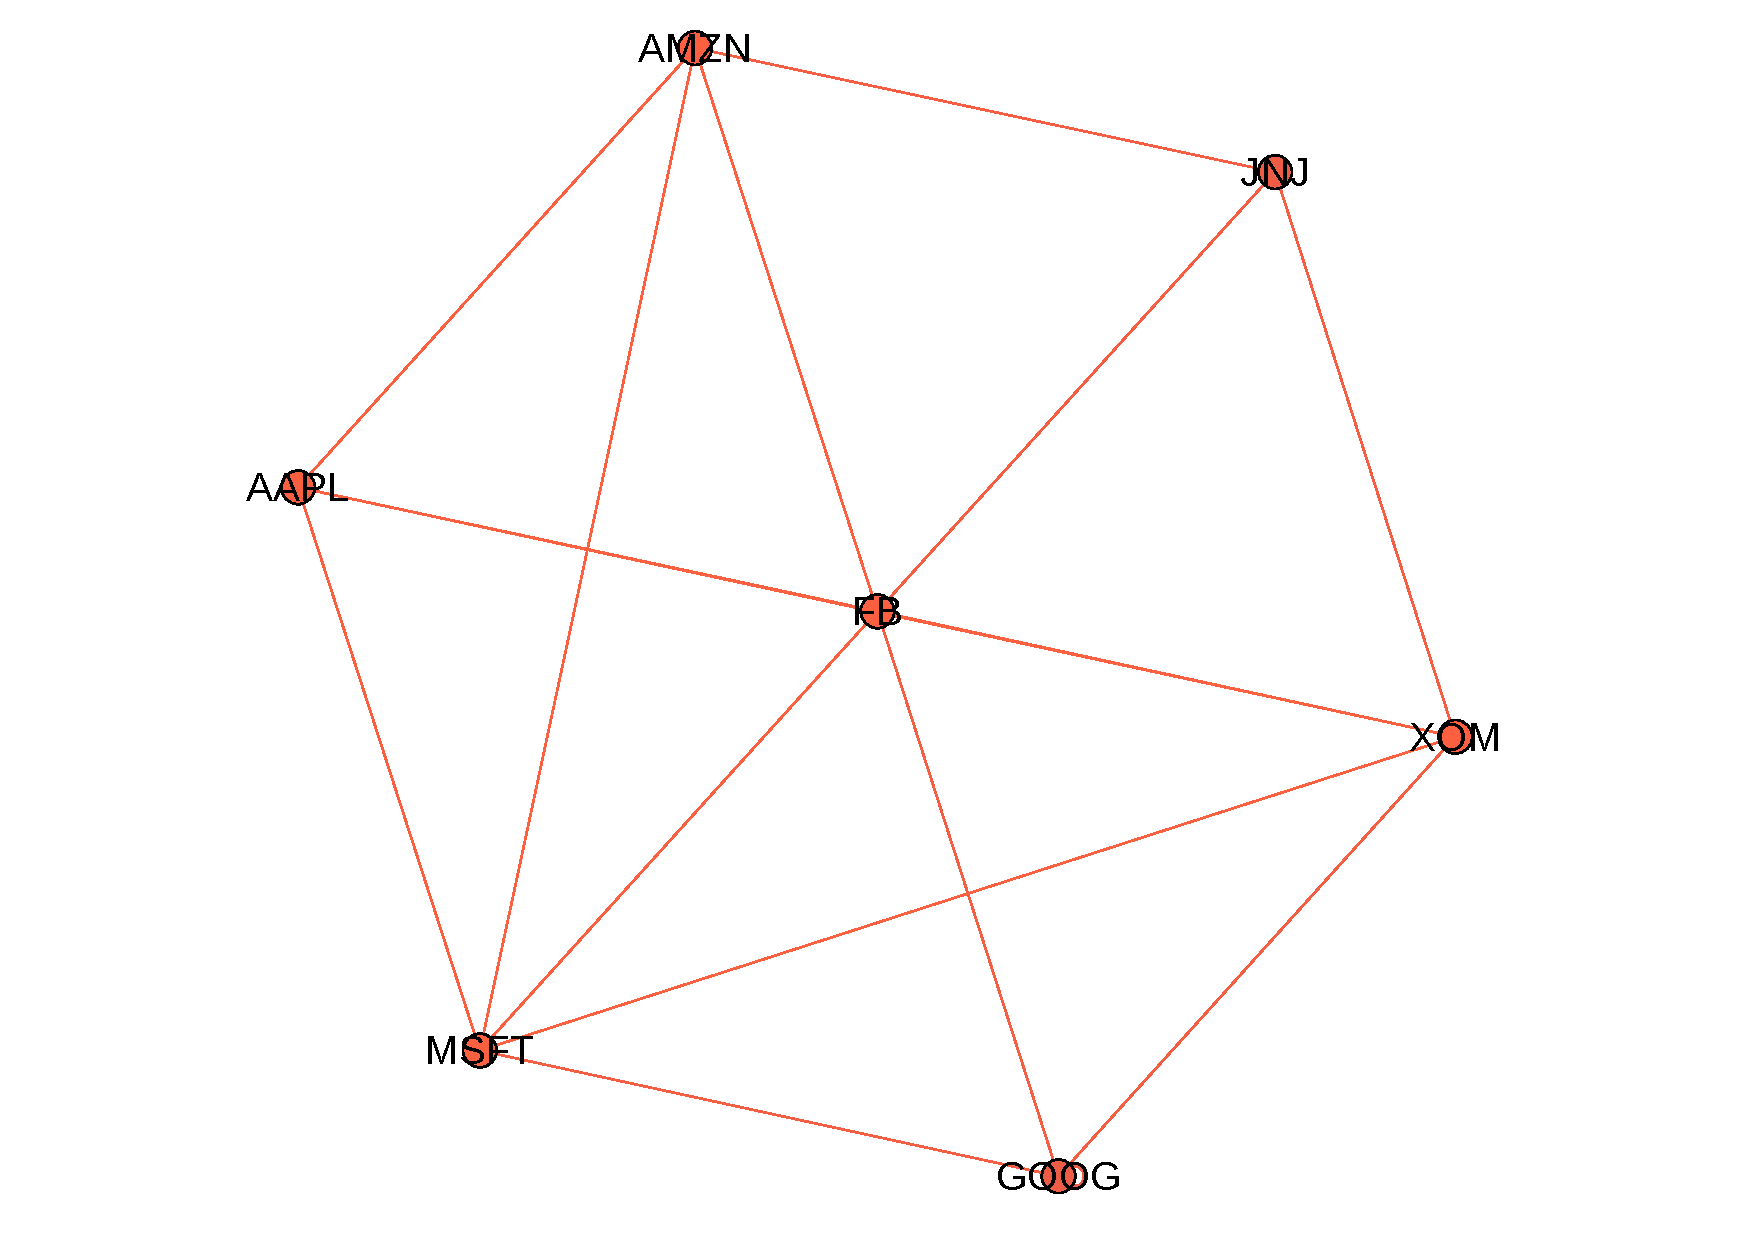
\includegraphics[width=\textwidth]{figures/Intro/ExampleNetwork.pdf}

      \caption{
      This figure contains an example of an undirected graph with 7 nodes and 16 edges. This graph is formed from randomly selecting stock symbol tickers from a set of tickers and forming connections randomly. The purpose of this data is solely to demonstrate the basics of network theory. The nodes are defined as circles and have ticker symbols overlaid on them. Edges are formed between nodes with lines between them. Since this is an undirected graph there is no directional information ergo no distinction as to whether one node is connected to another or vice-versa. The only information represented from an undirected graph is that they are connected. Lastly the amount of connections a node has is referred to as degree. So the node \(FB\) has 6 edges or a degree of 6.
      }
      \label{fig:ExampleNetwork}

  \end{figure*}

\begin{figure*}[!htb]
    \centering
     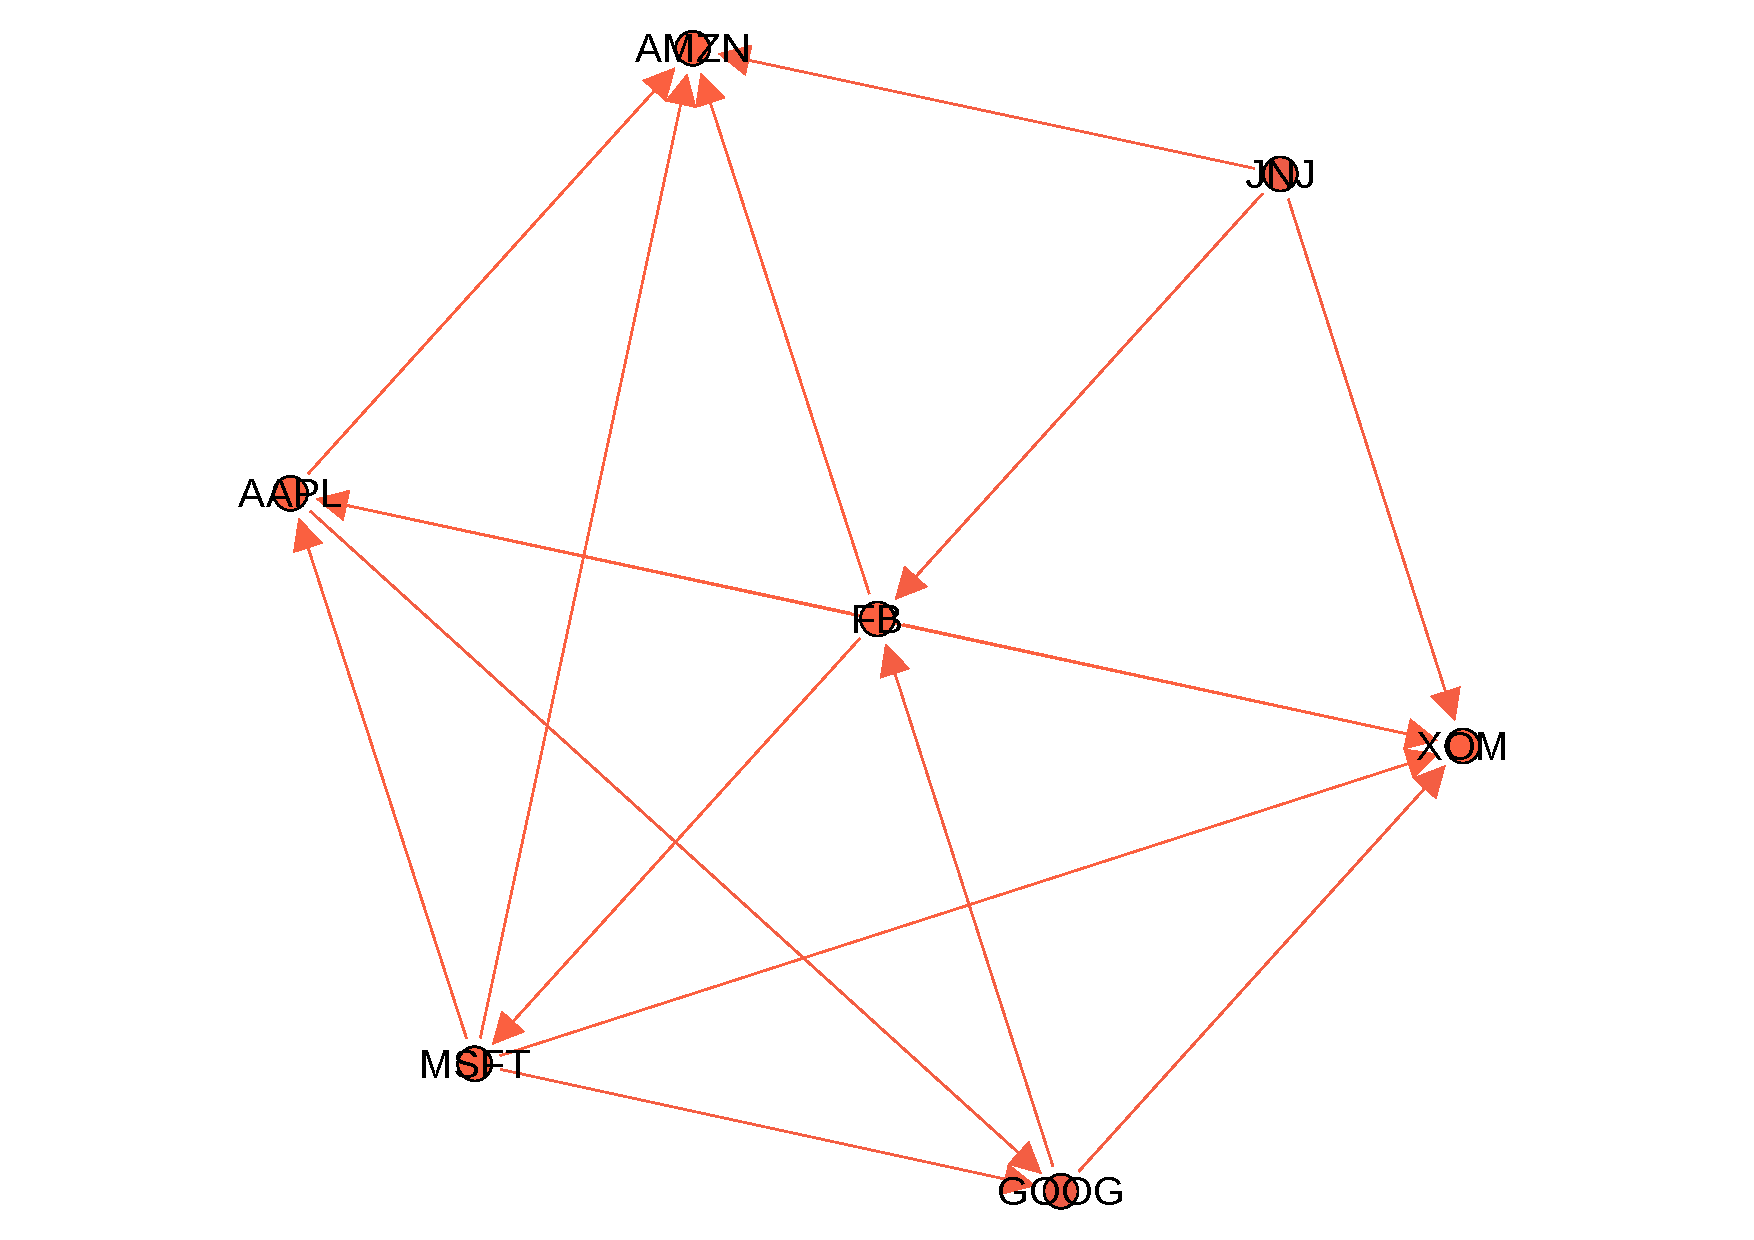
\includegraphics[width=\textwidth]{figures/Intro/ExampleNetworkDirected.pdf}
    \caption{
This graph is nearly identical to the graph in Figure \ref{fig:ExampleNetwork} except this graph is a directed network. This means that it contains directional information between the nodes. This directional information is communicated based on the position of the arrow in a line. For example, the node \(FB\) has an edge to \(MSFT\) however \(MSFT\) does not have an edge to \(FB\). The directional information allows other metrics to be used such as in-degree (which represents the amount of edges directed toward a node) and out-degree (which represents the amount of edges directed away from a node. In this example \(FB\) has an in-degree of 2, an out-degree of 4 and a degree of 6.
      }
	\label{fig:ExampleNetworkDirected}
\end{figure*}



  \begin{figure*}[!htb]
    \centering
      \centering
      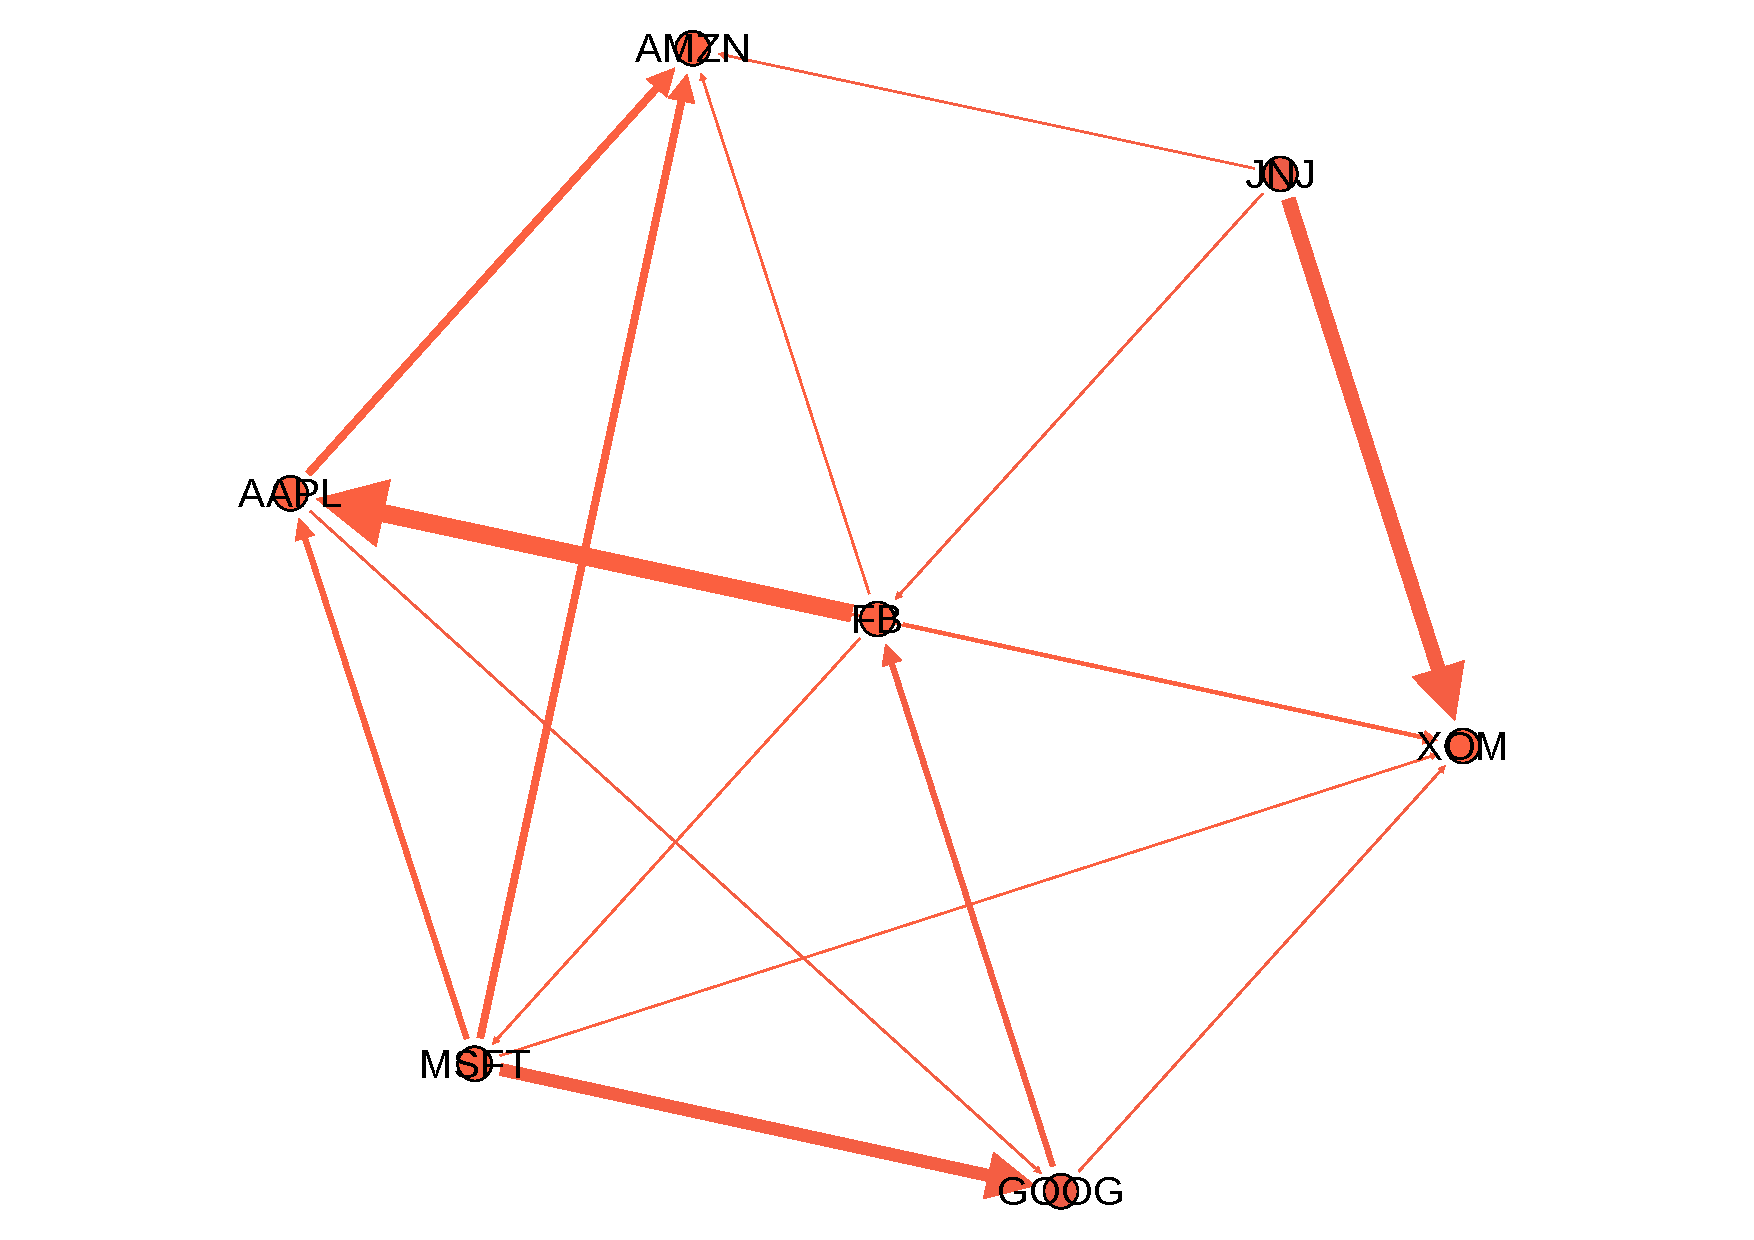
\includegraphics[width=\textwidth]{figures/Intro/ExampleNetworkDirectedWeighted.pdf}
      \caption{A nearly identical graph to the graph in Figure \ref{fig:ExampleNetworkDirected}. This directed graph contains weighted edges where a thick edge represents a high weight value (or strong connection). The smaller the edge weight value the thinner the edge will be.  Here \(FB\) has a strong connection to \(AAPL\) whereas \(FB\) has a weak connection to \(AMZN\).}
      \label{fig:ExampleNetworkDirectedWeighted}
    
  \end{figure*}

\begin{figure*}[!htb]
    \centering
      \centering
      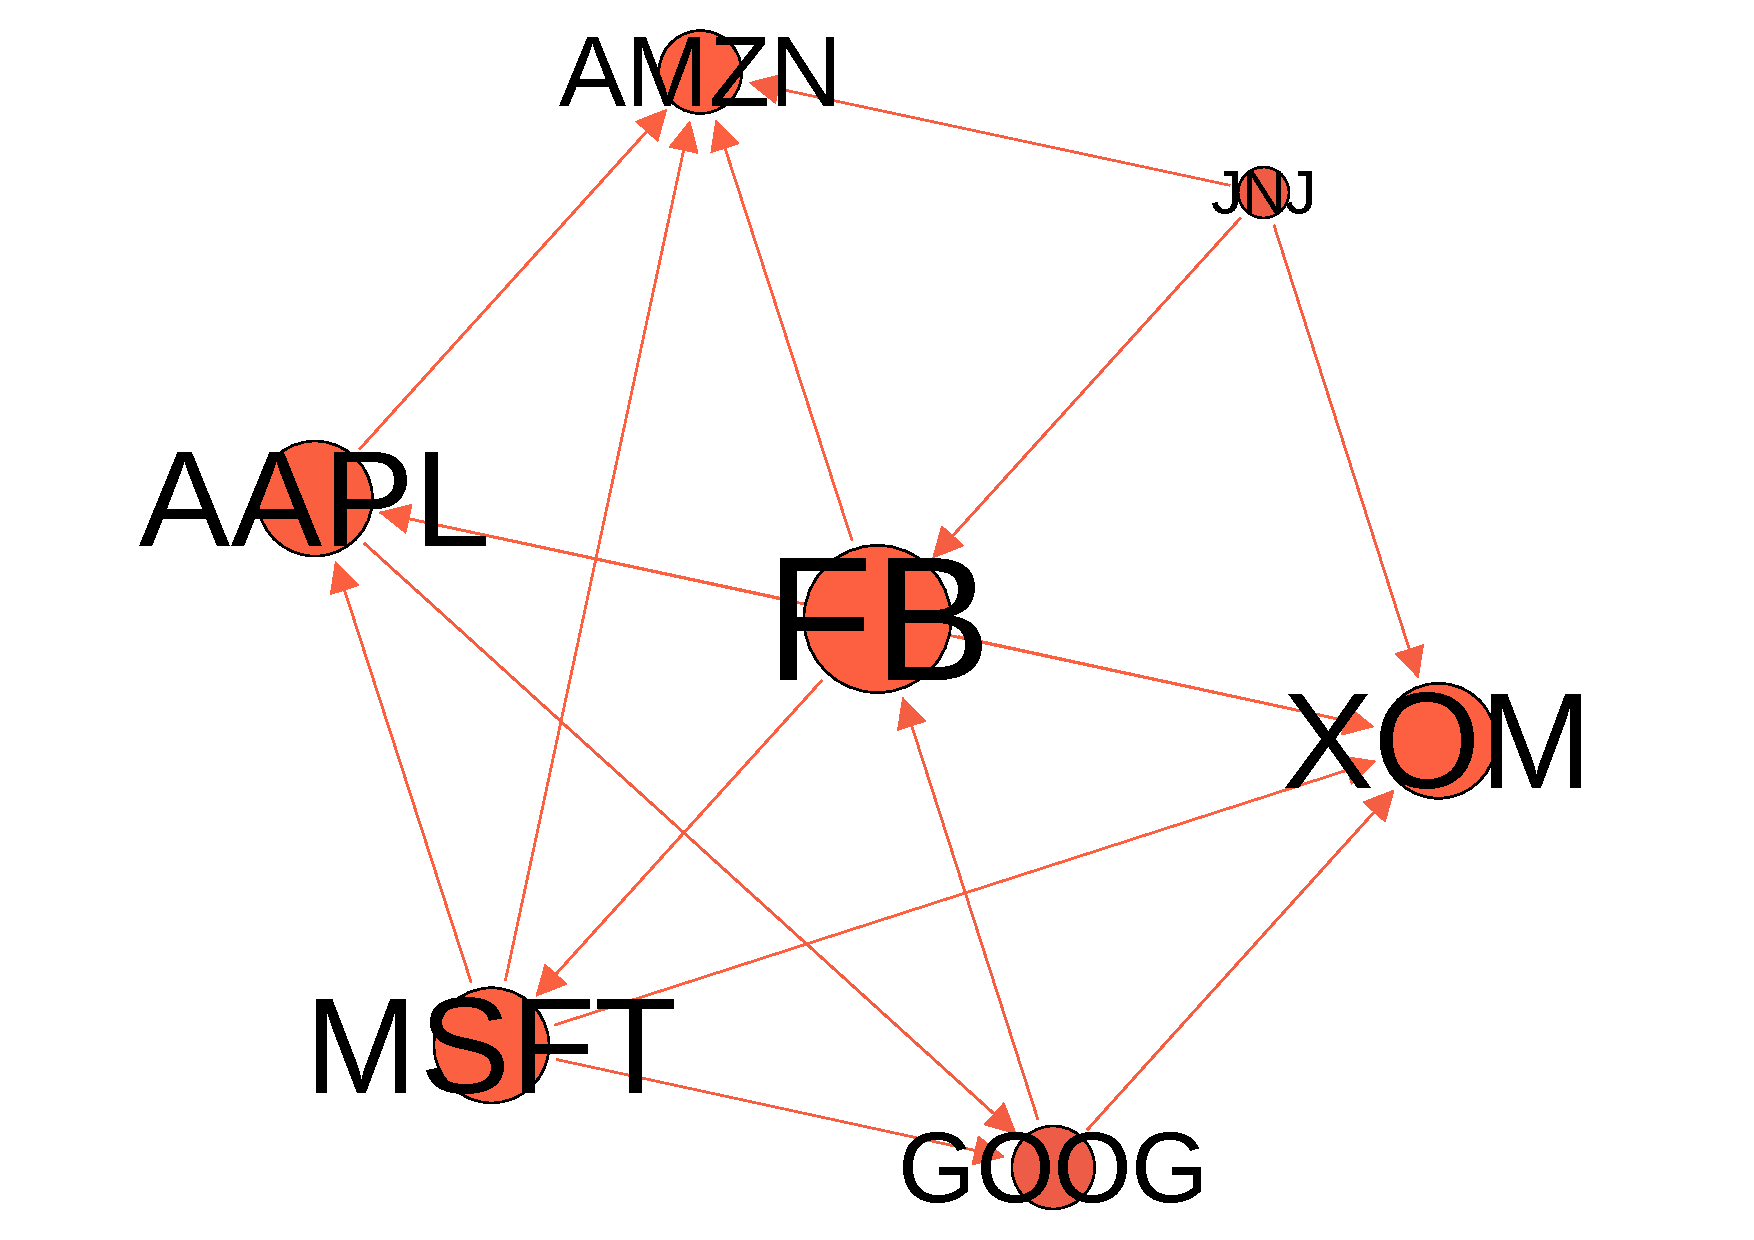
\includegraphics[width=\textwidth]{figures/Intro/ExampleNetworkDegree.pdf}
    \caption{
      A nearly identical graph to the graph in Figure \ref{fig:ExampleNetworkDirected}. Here the node sizes are scaled based on the degree. The higher the degree the larger the node size and consequently the smaller the degree the smaller the node size.
      }
      \label{fig:ExampleNetworkDegree}
  \end{figure*}


\begin{table}[htbp]
\begin{center}
    \begin{tabular}{|p{2cm}|p{1.5cm}|p{1.5cm}|p{1.5cm}|p{1.5cm}|p{1.5cm}|p{1.5cm}|p{1.5cm}|  }
        \hline
         & MSFT & AAPL & AMZN & FB & JNJ &  GOOG & XOM\\
        \hline
        MSFT  & 0 & 1 & 1 & 1  & 0 & 1 & 1 \\
        \hline
        AAPL & 1& 0 & 1 & 1 & 0 & 1 & 1 \\
        \hline
        AMZN & 1 & 1 & 0 & 1 & 1  & 0 & 0 \\
        \hline
        FB & 1 & 1 & 1 & 0  & 1 & 1 & 1 \\
        \hline
        JNJ & 0 & 0 & 1 & 1 & 0 & 0 & 0  \\ 
        \hline
        GOOG & 1 & 1 & 0 & 1 & 0 & 0 & 1 \\
        \hline
        XOM & 1 & 1 & 0 & 1 & 0 & 1 & 0  \\
        \hline
    \end{tabular}
\end{center}
\caption{ 
      This table contains an example of simulated data. This table was formed from randomly selecting stock symbol tickers from a set of tickers. The purpose of this data is solely to demonstrate the basics of network theory. Here the columns and row indicies belong to the selected tickers. The values contain either a 1 to represent if there is a connection between the ticker at a particular row index \(i\)  and the ticker of a particular column \(j\) or a 0 if there is no connection.
}

\label{tab:ExampleTable}
\end{table}

\begin{figure*}[!htb]
    \centering
      \centering
      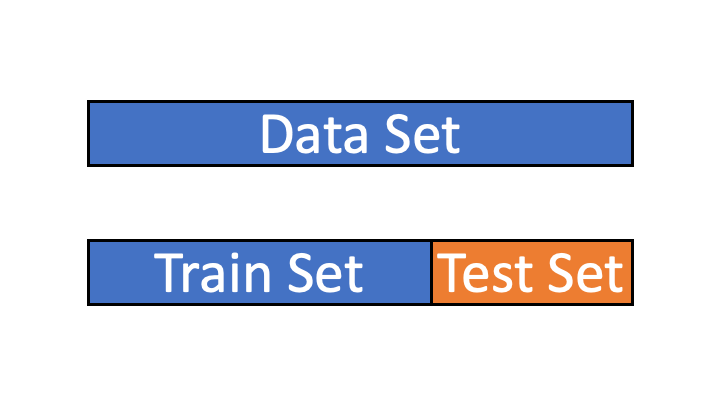
\includegraphics[width=\textwidth]{figures/ppt/TrainTestSplit.png}
    \caption{
      This figure shows how a data set can be partitioned for a supervised machine learning paradigm. The ``Data Set" is partitioned into 2 unequal sets with the``Train Set" having more data assigned to it than the ``Test Set". The ``Train Set" and ``Test Set" ratios can vary and is typically determined by the practitioner. There are many ways to partition the data for the train and test sets. For example the dataset can be partitioned sequentially from the data, or form partitions based on the data being randomly sampled.
      }
\label{fig:TrainTestSplit}

  \end{figure*}


\begin{figure*}[!htb]
    \centering
      \centering
      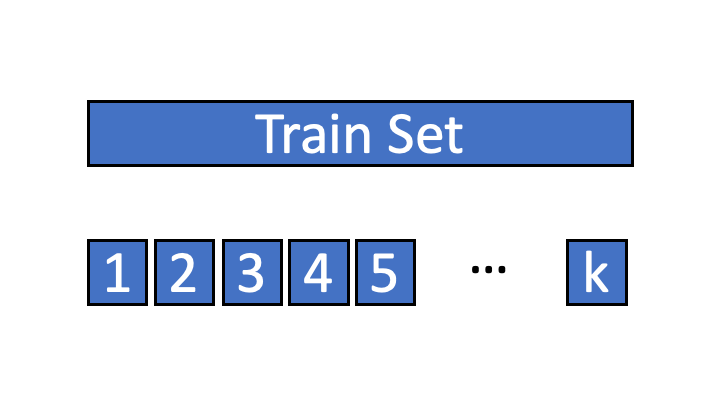
\includegraphics[width=\textwidth]{figures/ppt/KFoldValidation.png}
    \caption{
	``Train Set" here represents ``Train Set" in Figure \ref{fig:TrainTestSplit}. In this figure the data is split into \(k\) folds. How the \(k\) folds are created can vary. A common technique is to randomly divide the ``Train Set" observations into \(k\) equal folds.
      }
     \label{fig:KFoldValidation}
  \end{figure*}

\begin{figure*}[!htb]
    \centering
      \centering
      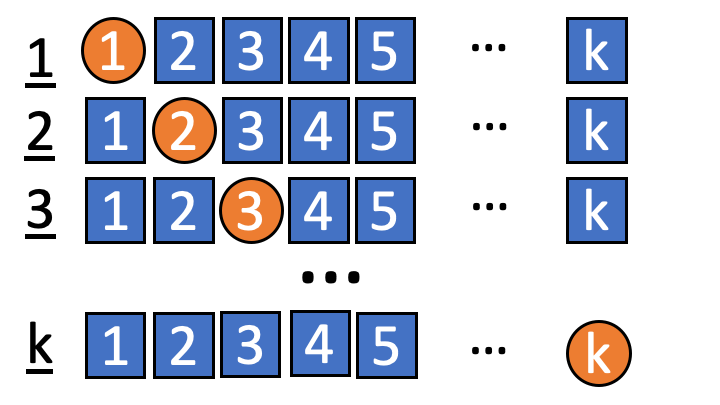
\includegraphics[width=\textwidth]{figures/ppt/KFoldValidationExplain.png}
     
    
    \caption{
	This figure breaks down how \(k\)-Fold Cross Validation works. These folds are created from ``Train Set" in Figure \ref{fig:KFoldValidation}. For the first iteration (where you see 1 underlined), the 1st fold (circle labeled 1) is used to assess the models ability and the remaining folds (squares) are used to train the model. The 2nd iteration follows the same procedure as the 1st except only the 2nd fold is withheld and the other folds are used. This repeats \(k\) times.
      }
\label{fig:KFoldValidationExplain}
  \end{figure*}


\begin{figure*}[!htb]
    \centering
      \centering
      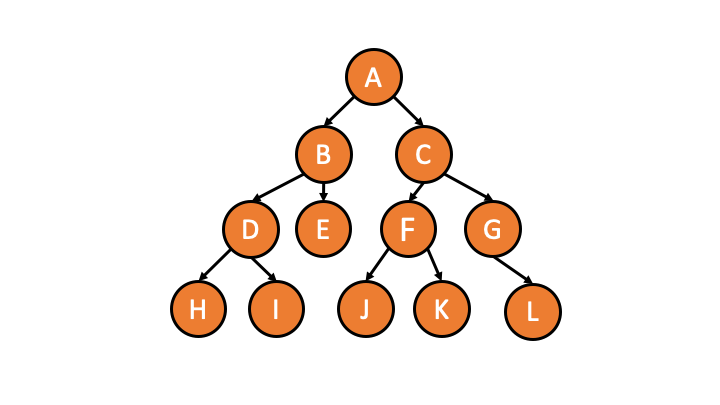
\includegraphics[width=\textwidth]{figures/ppt/DecisionTree.png}

    \caption{
	This figure shows an example of a Decision Tree. This is essentially a graph with no cycles.  Each circle represents a node (the label of the node is a letter inside of the node) and the arrows represent directional edges (branches) to another node. Node \(A\) is the root node of this tree and is where the decision begins. Potential outcomes from the root node lead to different states that are represented in nodes \(B\) and \(C\). \(B\) and \(C\) are the children of \(A\).  Nodes \(B\) and \(C\) have children and their children has children. Nodes \(H, I, E, J, K,\) and \(L\) are the leaf nodes of this tree because they have no children.
      }
      \label{fig:DecisionTree}
  \end{figure*}

\clearpage
\bibliographystyle{plainnat}
\bibliography{thesisbib}
\chapter{Standard Machine Learning Language}

\section{Introduction}
\label{Introduction}
\blfootnote{
This chapter contains material from the following working paper: 
\nobibliography{thesisbib}
\begin{itemize}
\item\bibentry{SML}
\end{itemize}
}
Machine Learning has simplified the process of solving problems in a variety of fields (see \cite{ML-UseCase1} or \cite{Monahan} for examples).  However \cite{pedros:fewUsefulThings} noted that there are a number of nuisances that should be taken into consideration when developing machine learning pipelines.  If these nuisances are not taken into consideration one may not receive satisfactory results.  To combat these issues we introduce Standard Machine Learning Language (SML) targeted at domain experts that want to utilize machine learning to solve research questions.

The overall objective of SML is to provide a level of abstraction which simplifies the development process of machine learning pipelines.  Consequently this enables students, researchers, and industry professionals without a background in developing machine learning pipelines to solve problems in different domains with machine learning (see Listing \ref{lst:sml-ex-1} for an example).  In the subsequent sections related works are discussed,  followed by defining the grammar used to create queries for SML. The architecture of SML is described,  lastly SML is applied to use-cases to demonstrate how it reduces the complexity of solving problems that utilize machine learning.

\section{Prior Works}
\label{SML:PriorWorks}

There are prior related works that attempt to provide a level of abstraction for developing machine learning models.  \cite{RizzoloRo10} created a tool called LBJava based on a programming paradigm called Learning Based Programming (see \cite{Roth05}). Learning Based Programming is an extension of conventional programming that creates functions using data driven approaches.  LBJava utilizes machine learning to create these functions and abstract the details from the user.  What differentiates SML from LBJava is that it offers a higher level of abstraction by providing a query like language which allows people who aren't experienced programmers to use SML.  

TPOT (see \cite{TPOT}) is a tool implemented in Python that creates and optimizes machine learning pipelines using genetic programming.  Given cleaned data,  TPOT  preprocessing the data,  performs feature selection,  and the construction of machine learning models.  Given the task (classification,  regression,  or clustering) TPOT uses genetic programming to tune model parameters and select features to determine the most optimal model to use.  Similar to TPOT \cite{kotthoff_auto_2019} developed Auto-WEKA which automates the selection of learning algorithms and tuning hyper-parameters for implemented models in WEKA see (\cite{frank2005weka}).   

Subsequently \cite{komer_hyperopt_2019} created Hyperopt-Sklearn that provides automated algorithm selection from models in the Scikit-learn machine learning library \footnote{See \cite{scikit-learn} for an introduction to Scikit-learn.} similar to Auto-Weka.  \cite{feurer_auto_2018} introduced improvements upon Hyperopt-Sklearn by taking into account past performance on similar datasets and constructing ensembles from optimized models.  %From the prior works,  it is probable to produce a model that will generalize well to new data; however it is likely that the model will be a black box not easily interpretable by the user.
What differentiates SML from these prior works is that it provides an agnostic language to reduce the amount programming that one has to write and offers a visualization framework to assess the models performance visually.

\section{Grammar}
\label{grammar}

The SML language is a domain specific language with grammar implemented in Bakus-Naur form (BNF) (see \cite{Backus59}).  Each expression has a rule and can be expanded into additional terms.  Listing \ref{lst:sml-ex-1} is an example of how one would perform classification on a dataset using SML. The query in listing \ref{lst:sml-ex-1} reads from a dataset, performs a 80/20 split of training and testing data respectively, and performs classification on the 5th column of the hypothetical dataset using columns 1,2,3, and 4 as predictors. In the subsequent subsections SML's grammar in BNF form is defined in addition to the keywords.

\subsection{Grammar Structure}
This subsection is dedicated to defining the grammar of SML in terms of BNF.  A \(Query\) can be defined by a delimited list of actions where the delimiter is an \(AND\) statement; with BNF syntax this is defined as:

\begin{equation} \label{BNF:Query}
<Query> ::= <Action> | <Action> AND <Query>
\end{equation}

An \(Action\) in (\ref{BNF:Query}) follows one of the following structures defined in (\ref{BNF:Action}) where a \(Keyword\) is required followed by an \(Argument\) and/or \(OptionList\).

\begin{equation} \label{BNF:Action}
\begin{split}
<Action> ::= <Keyword> <Argument> \\
| <Keyword> <Argument> (<Option List>) \\
| <Keyword> (<Option List>)
\end{split}
\end{equation}

A \(Keyword\) is a predefined term associating an \(Action\) with a particular string. An \(Argument\) generally is a single string surrounded by quotes that specifies a path to a file. Lastly,  an \(Argument\) can have a multitude of options (\ref{BNF:Option}) where an \(Option\) consist of an \(OptionName\) with either an \(OptionValue\) or \(OptionValueList\). An \(OptionName\) and \(OptionValue\) consist of a single string. An \(OptionList\) (\ref{BNF:OptionList}) consist of a comma delimited list of options and an \(OptionValueList\) (\ref{BNF:OptionValueList}) consist of a comma delimited list of \(OptionValues\).

\begin{equation} \label{BNF:Option}
\begin{split}
<Option> ::= <Option Name> = <Option Value> \\
		| <Option Name> = [<Option Value List>]
\end{split}
\end{equation}

\begin{equation} \label{BNF:OptionList}
\begin{split}
	<Option List> ::= <Option> | <Option>,  <Option List>
\end{split}
\end{equation}

\begin{equation} \label{BNF:OptionValueList}
\begin{split}
<Option Value List> ::= <Option Value> \\
| <Option Value> ,  <Option Value List>
\end{split}
\end{equation}

To put the grammar into perspective the example \(Query\) in Listing \ref{lst:sml-ex-1} has been transcribed into BNF format and can be found in Listing \ref{lst:SML:BNFComp}. In  Listing \ref{lst:SML:BNFComp}  the first \(Keyword\) is \(READ\) followed by an \(Arugment\) that specifies the path to the dataset. Next an \(OptionValueList\) contains information about the delimiter of the dataset and the header. We then include the \(AND\) delimiter to specify an additional \(Keyword\) \(SPLIT\) with an \(OptionValueList\) that tells us the size of the training and testing partitions for the dataset specified with the \(READ\) \(Keyword\). Lastly, the \(AND\) delimiter is used to specify another \(Keyword\) \(CLASSIFY\) which performs classification using the training and testing data from the result of the  \(SPLIT\) \(Keyword\) followed by an \(OptionValueList\) which provides information  to SML about the features to use (columns 1-4), the label we want to predict (column 5), and the algorithm to use for classification. The next subsection describes the functionality for all \(Keyword\)s of SML.

\subsection{Keywords}
Currently there are 8 \(Keyword\)s in SML \footnote{Detailed documentation providing examples and describing all of the keywords of SML are publicly available on github: https://github.com/lcdm-uiuc/sml/tree/master/dataflows \label{SML:Dataflow}}. These \(Keyword\)s can be chained together to perform a variety of actions. In the subsequent subsections we describe the functionality of each \(Keyword\).

\subsubsection{Reading Datasets}
When reading data from SML one must use the \(READ\) \(Keyword\) followed by an \(Argument\) containing a path to the dataset. \(READ\) also accepts a variety of \(Option\)s. The first \(Query\) in listing \ref{lst:SML:READ} consist of only a \(Keyword\) and \(Argument\). This \(Query\) reads in data from "/path/to/dataset". The second \(Query\) includes an \(OptionValueList\) in addition to reading data from the specified path; the \(OptionValueList\) specifies that the dataset is delimited with semicolons and does not include a header row. 


\subsubsection{Cleaning Data}
When NaNs, NAs and/or other missing values are present in dataset we clean these values in SML by using the \(REPLACE\) \(Keyword\).  Listing \ref{lst:SML:REPLACE}  shows an example of the \(REPLACE\) \(Keyword\) being used. In this \(Query\) we use the \(REPLACE\) \(Keyword\) in conjunction with the \(READ\) \(Keyword\).  SML reads from a comma delimited dataset with no header from the path "/path/to/dataset". Then we replace any instance of "NaN" with the mode of that column in the dataset.


\subsubsection{Partitioning Datasets}
It's often useful to split a dataset into training and testing datasets for most tasks involving machine learning.  This can be achieved in SML by using the \(SPLIT\) \(Keyword\).  Listing \ref{lst:SML:SPLIT} shows an example of a SML \(Query\) performing a 80/20 split for training and testing data respectively by utilizing the \(SPLIT\) \(Keyword\) after reading in data.

\subsubsection{Creating Models}

In SML,  one can create create a model to either perform classification, regression, or clustering. To use a classification model in SML one would use the \(CLASSIFY\) \(Keyword\). SML has the following classification models implemented: Support Vector Machines, Naive Bayes, Random Forest, Logistic Regression, and K-Nearest Neighbors.  Listing \ref{lst:SML:CLASSIFY} demonstrates how to use the \(CLASSIFY\) \(Keyword\) in a \(Query\).  Clustering models can be utilized by using the \(CLUSTER\) \(Keyword\).  SML currently has K-Means clustering implemented.  Listing \ref{lst:SML:CLUSTER} demonstrates how to use the \(CLUSTER\) \(Keyword\) in a \(Query\).  Regression models use the \(REGRESS\) \(Keyword\).  SML currently has the following regression algorithms implemented: Simple Linear Regression, Ridge Regression, Lasso Regression, and Elastic Net Regression. Listing \ref{lst:SML:REGRESS} demonstrates how to use the \(REGRESS\) \(Keyword\) in a \(Query\).


\subsubsection{Saving/Loading Models}
It's possible to save models and reuse them later. To save a model in SML one would use the \(SAVE\) \(Keyword\) in a \(Query\). To load an existing model from SML one would use the \(LOAD\) \(Keyword\) in a \(Query\).  Listing \ref{lst:SML:SAVE_LOAD} shows the syntax required to save and load a model using SML.  With any of the existing queries using \(REGRESS\),  \(CLUSTER\),  or \(CLASSIFY\) \(Keyword\)s attaching \(SAVE\) to the \(Query\) will save the model. 

\subsubsection{Visualizing Datasets and Metrics of Algorithms}
When using SML it's possible to visualize datasets or performance of models (such as learning curves or ROC curves).  To do this the \(PLOT\) \(Keyword\) must be specified in a \(Query\).  Listing \ref{lst:SML:PLOT} shows an example of how to use the \(PLOT\) \(Keyword\) in a \(Query\).  We apply the same operations to perform clustering in Listing \ref{lst:SML:CLUSTER} however we utilize the \(PLOT\) \(Keyword\).

\section{SML's Architecture}
\label{sml-architecture}

With SML's grammar defined, enough information has been presented to explain SML's architecture.  When SML receives a \(Query\) in the form of a string, it is passed to the parser. The grammar is then used to parse through the string to determine the actions to perform.  The actions are stored in a dictionary and given to one of the following phases of SML: Model Phase, Apply Phase, or Metrics Phase. Figure \ref{fig:SML:Architecture} shows a block diagram of this process.

The model phase is for constructing a model. The \(Keyword\)s that generally invoke the model phase are: \(READ\), \(REPLACE\), \(CLASSIFY\), \(REGRESS\), \(CLUSTER\), and \(SAVE\). The apply phase is  for applying a preexisting model  to new data. The \(Keyword\) that  invokes the apply phase is \(LOAD\). It's often useful to visualize the data that one works with and beneficial to see performance metrics of a machine learning model. By default if you specify the \(PLOT\) \(Keyword\) in a \(Query\), SML will execute the metrics phase.

The last significant component of SML's architecture is the connector. The connector connects drivers from different libraries and languages to achieve an action a user wants during a particular phase (see Figure \ref{fig:SML:Connector}). If one considers applying linear regression on a dataset, during the model phase SML calls the connector to retrieve the linear regression library in this case SML uses sci-kit learn's implementation however, if we wanted to use an algorithm not available in sci-kit learn such as a Hidden Markov Model (HMM) SML will use the connector to call another library that supports HMM.

\section{Interface}
\label{interface}

They're multiple interfaces available for working with SML. We have developed an alpha version of a web tool  which allows users to write queries and get results back from SML through a web interface (see Figure \ref{fig:SML:website}). There's also a REPL environment available that allows the user to interactively write queries and displays results from the appropriate phases of SML.  Lastly,  users have the option to import SML into an existing pipeline to simplify the development process of apply machine learning to problems.

\section{Use Cases}
\label{use-cases}

We tested SML's framework against ten popular machine learning problems with publicly available data sets. We applied SML to the following datasets: Iris Dataset \footnote{https://archive.ics.uci.edu/ml/datasets/Iris}, Auto-MPG Dataset \footnote{https://archive.ics.uci.edu/ml/datasets/Auto+MPG}, Seeds Dataset \footnote{https://archive.ics.uci.edu/ml/datasets/seeds},  Computer Hardware Dataset \footnote{https://archive.ics.uci.edu/ml/datasets/Computer+Hardware},  Boston Housing Dataset \footnote{https://archive.ics.uci.edu/ml/datasets/Housing}, Wine Recognition Dataset \footnote{https://archive.ics.uci.edu/ml/datasets/Wine}, US Census Dataset \footnote{https://archive.ics.uci.edu/ml/datasets/US+Census+Data+(1990)}, Chronic Kidney Disease \footnote{https://archive.ics.uci.edu/ml/datasets/Chronic\_Kidney\_Disease}, Spam Detection \footnote{https://archive.ics.uci.edu/ml/datasets/Spambase} which were taken from UCI's Machine Learning Repository (see \cite{Lichman:2013}).  We also applied SML to the Titanic Dataset \footnote{https://www.kaggle.com/c/titanic}.  

As mentioned in footnote \ref{SML:Dataflow} there are detailed examples and explanations for all 10 data sets.  In this paper we discuss in detail the process of applying SML to the Iris Dataset and the Auto-MPG dataset.   In particular we compare the process for using machine learning to solve the problems presented by the datasets with SML against traditionally writing code.  We forgo comparing SML to prior works in section \ref{SML:PriorWorks}.  For both of these data sets we used the same libraries and programming language in SML for writing code to solve these use cases. 

\subsubsection{Iris Dataset}
Listing \ref{lst:SML:IrisQuery} shows all of the code required to perform classification on the Iris dataset using SML in Python.  In listing \ref{lst:SML:IrisQuery} data is read in from a specified path named "iris.csv" of a subdirectory called "data". performs a 80/20 split, uses the first 4 columns to predict the 5th column, uses support vector machines as the algorithm to perform classification and finally plot distributions of features from the dataset and metrics of the classification model's performance.  Appendix A illustrates what is required to perform the same operations using Python and sci-kit learn.  The \(Query\) in listing \ref{lst:SML:IrisQuery} and the code in Appendix A use the same 3rd party libraries implicitly or explicitly.  It's also worth noting that the code in Appendix A is publicly available and well documented \footnote{For a detailed documentation describing this code visit: https://github.com/lcdm-uiuc/sml/blob/master/dataflows/plot/iris\_svm-READ-SPLIT-CLASSIFY-PLOT.ipynb \label{lab:iris:git}} and it is out of the scope of this paper.  Instead the complexities required to produce such results with and without SML are outlined.  The result for both snippets of code are the same and can be seen in Figure \ref{fig:IrisResults}.

\subsubsection{Auto-Mpg Dataset}
Listing  \ref{lst:SML:AutoMPGQuery} shows the SML \(Query\) required to perform regression on the Auto-MPG dataset in Python.  In listing \ref{lst:SML:AutoMPGQuery} we read data from a specified path, the dataset is separated by fixed width spaces and we choose not to provide a header for the dataset.  Next we perform a 80/20 split, replace all occurrences of "?" with the mode of the column. We then perform linear regression using columns 2-8 to predict the 1st label. Lastly, we visualize distributions of features from the dataset and metrics of our algorithm.  Appendix B.  demonstrates what's required to perform the same operations using scikit learn \footnote{For a detailed documentation describing this code visit: https://github.com/lcdm-uiuc/sml/blob/master/dataflows/plot/autompg\_linear\_regression-READ-SPLIT-REGRESS-PLOT.ipynb \label{lab:SML:AUTO}}. The outcome of both processes are the same and can be seen in Figure \ref{fig:AutoMPG:Results}.

\subsection{Discussion}
For the Iris and Auto-MPG use cases the same libraries and programming language were used to perform regression and classification.  The amount of work required to perform a task and produce the following results in Figure \ref{fig:AutoMPG:Results} and Figure \ref{fig:IrisResults} significantly decreases when SML is utilized.  Constructing each SML query used less than 10 lines of code however, implementing the same procedures without SML using the same programming language and libraries needed 70+ lines of code.  This provides evidence that SML simplifies the development process of solving problems with machine learning.  

\section{Future Work}
While we have formally introduced an agnostic framework a lot of work remains to be done to improve SML.  In the future we plan to extend the connector to support more machine learning libraries and additional languages.  SML's web application can be extended out to include additional functionality to improve the ease of use.  Feature selection, model selection, and parameter optimization are additional areas to add to SML.  In addition to improving SML it can also be tested by researchers in a comparative analysis against the works outlined in section \ref{SML:PriorWorks} to determine how beneficial SML is against alternative frameworks.

\section{Conclusion}
\label{conclusion}
To summarize we introduced an agnostic framework that integrates a query-like language to simplify the development of machine learning pipelines.  We provided a high level overview of it's architecture and grammar. We then applied SML to machine learning problems and demonstrated how the amount of the code one has to write significantly decreases when SML is used.  The source code and detailed documentation for SML is open-sourced and publicly available on github \footnote{https://github.com/lcdm-uiuc/sml \label{SML:Github}}. 


SML provides a realm of possibility to rapidly develop machine learning pipelines with an agnostic language to solve problems. This attractive aspect can boost  the productivity of researchers which utilize machine learning.  Abstracting the complexities of machine learning with a tool like SML can foster new research and solve problems in different disciplines at a faster rate.

\clearpage

\section{Figures and Listings}

\subsection{Figures}
\begin{sidewaysfigure}[!h]
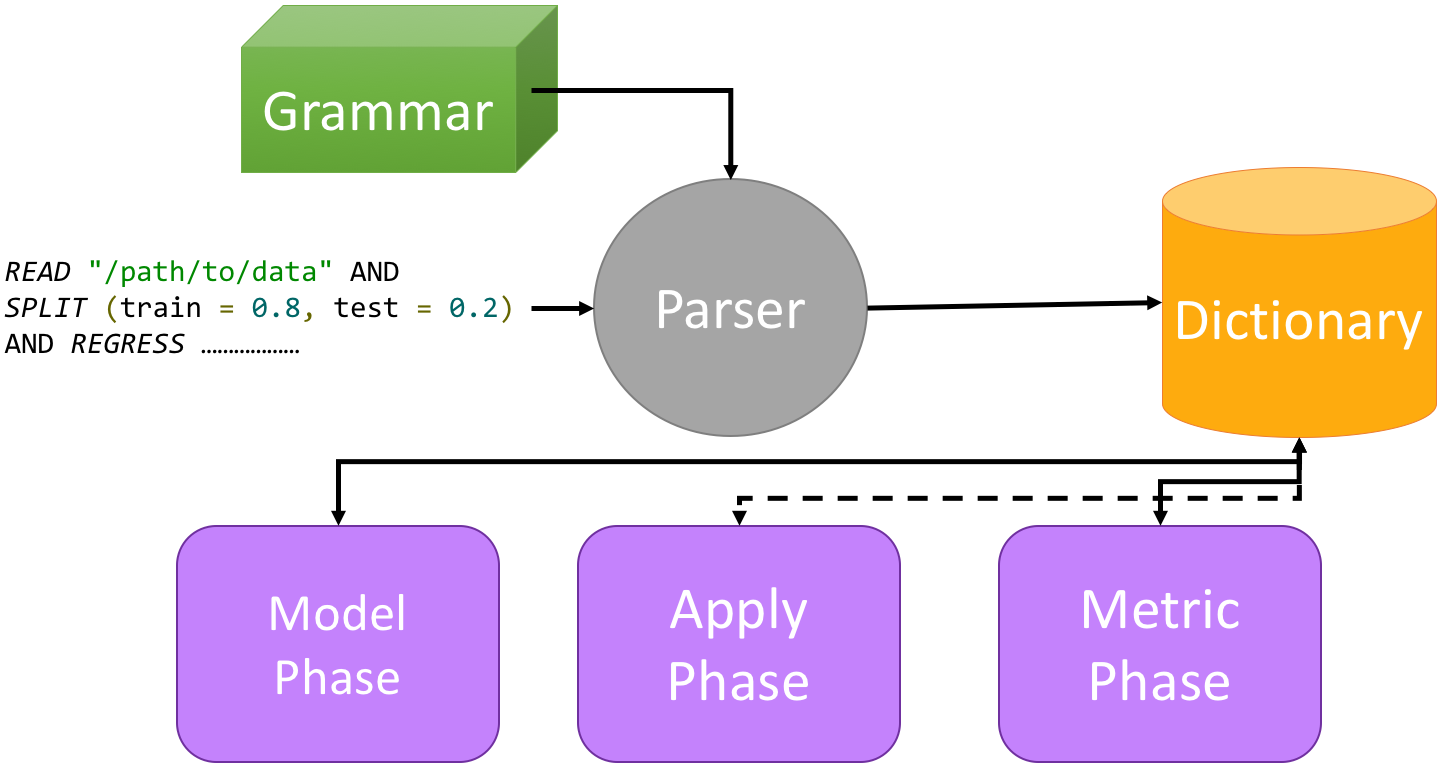
\includegraphics[width=.9\textwidth]{figures/SML/architecture.png}
\centering
\caption{Block Diagram of SML's Architecture\\}
\label{fig:SML:Architecture}
\end{sidewaysfigure}

\begin{sidewaysfigure}![h]
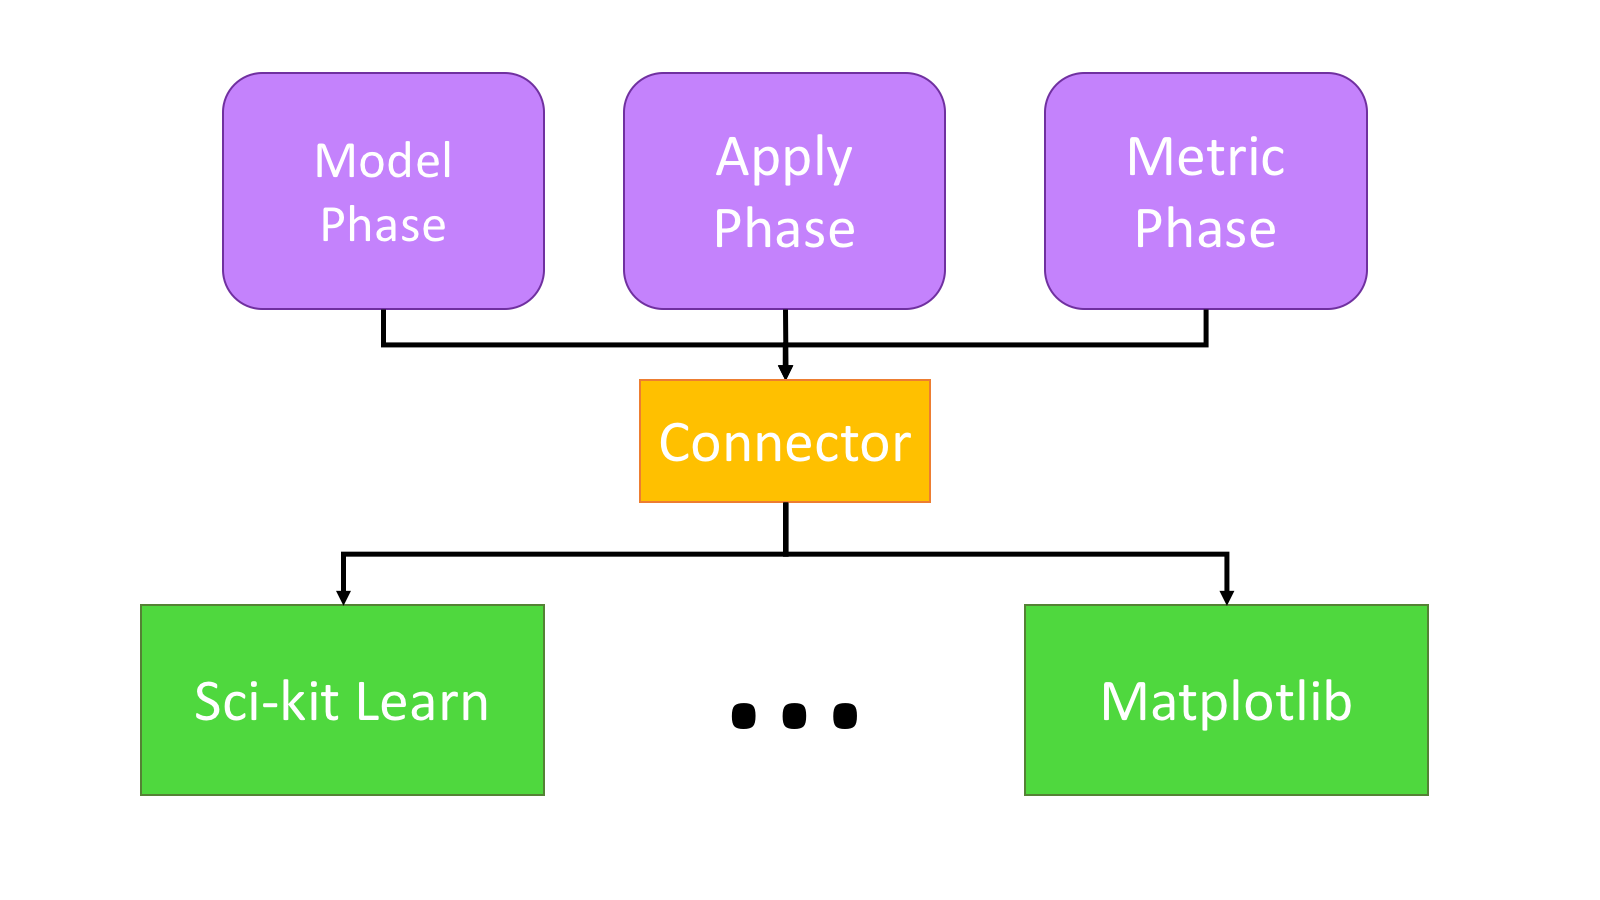
\includegraphics[width=1\textwidth]{figures/SML/connector.png}
\centering
\caption{Block Diagram of SML's Connector\\}
\label{fig:SML:Connector}
\end{sidewaysfigure}

\begin{sidewaysfigure}[!h]
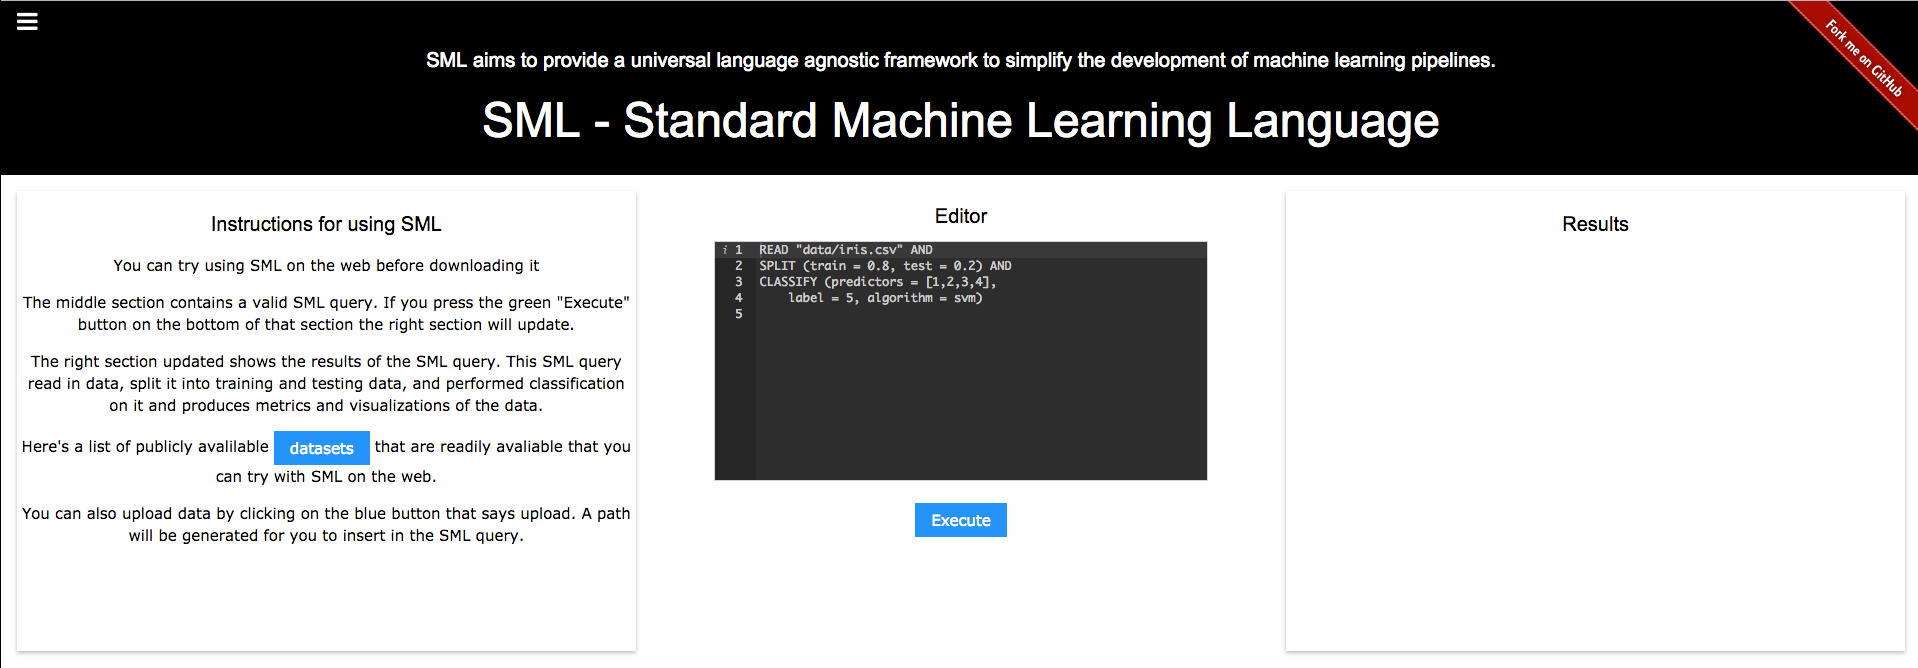
\includegraphics[width=1\textwidth]{figures/SML/sml-web-site.png}
\centering
\caption{Interface of SML's website. Currently users can read instructions and examples of how to use SML are on the left pane. In the middle pane users can type an SML \(Query\) and then hit the execute button. The results of running the \(Query\) through SML are then displayed on the right pane.\\}
\label{fig:SML:website}
\end{sidewaysfigure}


\begin{sidewaysfigure}[!h]
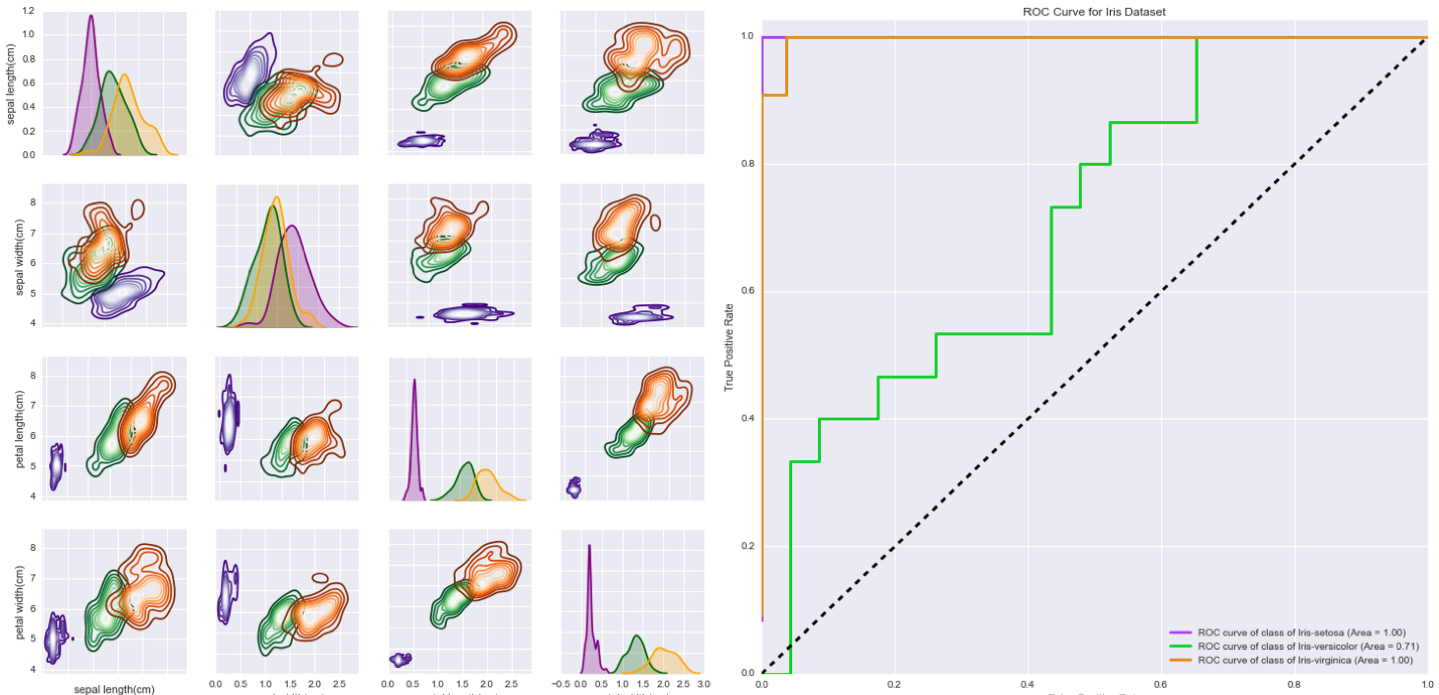
\includegraphics[width=1\textwidth]{figures/SML/iris_results.png}
\centering
\caption{The SML \(Query\) in Figure \ref{fig:SML:IrisQuery} and the code in Figure \ref{fig:Manual:IrisCode} produce these results. The subgraph on the left is a lattice plot showing the density estimates of each feature used. The graph on the right shows the ROC curves for each class of the iris dataset.\\}
\label{fig:IrisResults}
\end{sidewaysfigure}

\begin{sidewaysfigure}[!h]
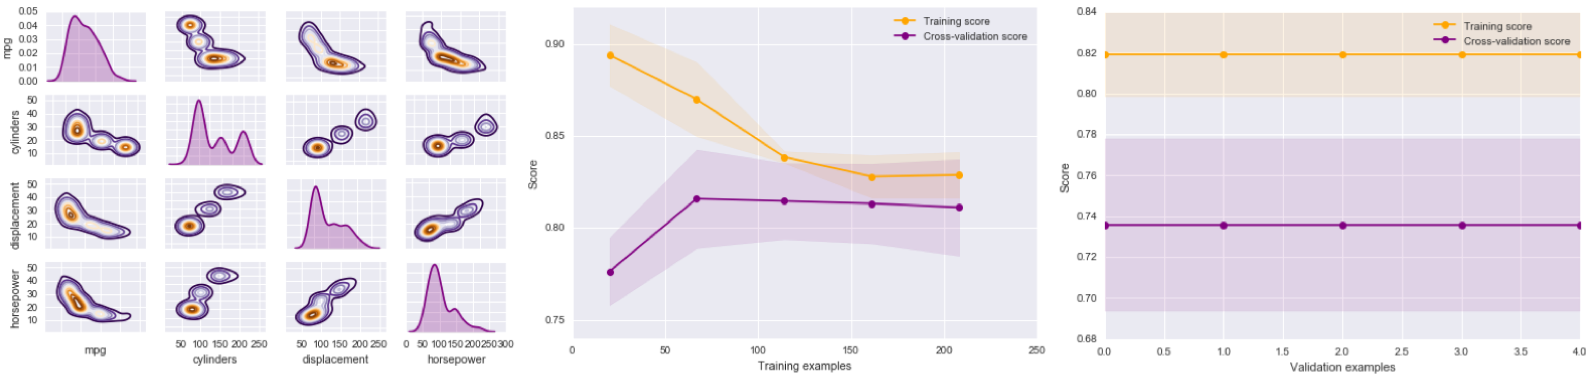
\includegraphics[width=1\textwidth]{figures/SML/auto-mpg-results.png}
\centering
\caption{The SML \(Query\) in Figure \ref{fig:SML:AutoMPGQuery}  and the code in Appendix B. produce these results. The subgraph on the left is a lattice plot showing the density estimates of each feature used. The top right graph shows the learning curve of the model and the graph on lower right shows the validation curve.\\}
\label{fig:AutoMPG:Results}
\end{sidewaysfigure}

\clearpage


\subsection{Listings}
\begin{lstlisting}[language=python,  caption={Example of a SML Query Performing Classification.}, label={lst:sml-ex-1}]
READ "/path/to/data" (separator =  ";", header = None) 
AND SPLIT (train = 0.8,  test=0.2) AND CLASSIFY 
(predictors =[1,2,3,4],  label = 5, algorithm = svm) 
\end{lstlisting}


\begin{lstlisting}[language=python,  caption={Here the example \(Query\) in listing \ref{lst:sml-ex-1} is defined in BNF format.}, label={lst:SML:BNFComp}]
<Keyword> <Argument> (<OptionList>) 
AND <Keyword> (<OptionList>) AND <Keyword>
(<OptionList>) 
\end{lstlisting}

\begin{lstlisting}[language=python,  caption={Examples using the \(READ\) \(Keyword\) in SML.}, label={lst:SML:READ}]
READ "/path/to/data" 
READ "/path/to/data" (separator = ";", header = None) 
\end{lstlisting}


\begin{lstlisting}[language=python,  caption={An example utilizing the \(REPLACE\) \(Keyword\) in SML.}, label={lst:SML:REPLACE}]
READ "/path/to/data" (separator = ";", header = None) 
AND REPLACE (missing = "NaN",  strategy = "mode")
\end{lstlisting}

\begin{lstlisting}[language=python,  caption={Example using the \(SPLIT\) \(Keyword\) in SML.}, label={lst:SML:SPLIT}]
READ "/path/to/data" (separator = ";", header = None) 
AND SPLIT (train = 0.8, test = 0.2)
\end{lstlisting}

\begin{lstlisting}[language=python,  caption={Example using the \(CLASSIFY\) \(Keyword\) in SML.  Here we read in data and create training and testing datasets using the \(READ\) and \(SPLIT\) \(Keyword\)s respectively. We then use \(CLASSIFY\) \(Keyword\) with the first 4 columns as features and the 5th column to perform classification using a support vector machine.}, label={lst:SML:CLASSIFY}]
READ "/path/to/data" (separator = ";", header = None) 
AND SPLIT (train = 0.8, test = 0.2) AND CLASSIFY
(predictors = [1,2,3,4],  label=5,  algorithm=svm)
\end{lstlisting}

\begin{lstlisting}[language=python,  caption={Example using the CLUSTER Keyword in SML. Here we read in data and create training and testing datasets using the READ and SPLIT Keywords respectively. We then use CLUSTER Keyword with the first 4 columns as features and perform unsupervised clustering with the K-Means algorithm.}, label={lst:SML:CLUSTER}]
READ "/path/to/data" (separator = ";", header = None) 
AND SPLIT (train = 0.8, test = 0.2) AND  CLUSTER
(predictors = [1,2,3,4],  algorithm=kmeans)
\end{lstlisting}

\begin{lstlisting}[language=python,  caption={Example using the \(REGRESS\) \(Keyword\) in SML. Here we read in data and create training and testing datasets using the \(READ\) and \(SPLIT\) \(Keyword\)s respectively. We then use \(REGRESS\) \(Keyword\) with the first 4 columns as features and the 5th column to perform regression on using ridge regression.}, label={lst:SML:REGRESS}]
READ "/path/to/data" (separator = ";", header = None) 
AND SPLIT (train = 0.8, test = 0.2) AND  CLUSTER
(predictors = [1,2,3,4],  label=5, algorithm=ridge)
\end{lstlisting}

\begin{lstlisting}[language=python,  caption={Example using the \(LOAD\) and \(SAVE\) \(Keyword\)s in SML.}, label={lst:SML:SAVE_LOAD}]
SAVE "/path/to/save/model" 
LOAD "/path/to/save/model" 
\end{lstlisting}

\begin{lstlisting}[language=python,  caption={Example using the \(PLOT\) \(Keyword\) in SML.}, label={lst:SML:PLOT}]
READ "/path/to/data" (separator = ";", header = None) 
AND SPLIT (train = 0.8, test = 0.2) AND  CLUSTER
(predictors = [1,2,3,4],  algorithm=kmeans)
AND PLOT
\end{lstlisting}

\begin{lstlisting}[language=python,  caption={SML \(Query\) that performs classification on the iris dataset using support vector machines. It's important to note that detailed documentation is publicly available in \textsuperscript{\ref{lab:iris:git}} and the purpose of this figure is to highlight the level of the level of complexity relative to an SML query.}, label={lst:SML:IrisQuery}]
from sml import execute
query = 'READ "../data/iris.csv" AND \ 
SPLIT (train = 0.8, test = 0.2) AND \ 
CLASSIFY (predictors = [1,2,3,4],  label = 5, algorithm=svm) AND \
PLOT'

execute(query, verbose=True)
\end{lstlisting}

\begin{lstlisting}[language=python,  caption={SML \(Query\) that performs regression on the Auto-MPG dataset using Linear Regression.}, label={lst:SML:AutoMPGQuery}]
from sml import execute
query = 'READ "../data/auto-mpg.csv" AND \ 
REPLACE (missing = "?", strategy = "mode") AND \
SPLIT (train = 0.8, test = 0.2) AND \ 
REGRESS (predictors = [2,3,4,5,6,7,8],  label = 1, algorithm=simple) AND \
PLOT'

execute(query, verbose=True)
\end{lstlisting}



\clearpage

%\appendix


\clearpage
\bibliographystyle{plainnat}
\bibliography{thesisbib}
%\chapter{Predicting Profitability Using Machine Learning}
\chapter{Directional Profitability Predictions with Random Forests} \label{Chapter:ABIS}

\section{Introduction}
\blfootnote{
	This chapter contains material from the following working paper: 
	\nobibliography{thesisbib}
	\begin{itemize}
		\item\bibentry{ABIS}
	\end{itemize}
}

\RC{This first statement should be clarified. Not all countries/people would agree.}

An economic goal of a society is to maximize wealth. In order to maximize wealth, resources such as labor, capital, and natural resources must be allocated efficiently to firms. Capital markets (such as the stock market) allow capital to be efficiently allocated to said firms. Firm profitability can affect society, whether through job growth or loss, the offered services, the provision of goods, or personal gain or loss (see \cite{IntAccBook}).  Predicting the future profitability for firms is an essential endeavor as it is central to the valuation of the firm and the securities they issue (see \cite{Monahan}). 

A study by \cite{Bradshaw} provides evidence that analysts' predictions are not superior to random walk predictions, indicating that traditional methods provide little efficacy. \cite{Monahan} conducts a review and discussion on the accounting research related to out-of-sample profitability predictions.  He provides evidence that models in prior works have lower out-of-sample accuracy than random walk models. This provides motivation to seek an alternative method, given the shortcomings of traditional methods.   \cite{ABIS:ML:EX1},  \cite{ABIS:ML:EX2},  \cite{ABIS:ML:EX3},  and \cite{ABIS:ML:EX4} are relatively recent examples that demonstrate the effectiveness of machine learning for prediction and inference in a variety of applications.  Thus, we explore machine learning methods to predict the future profitability of firms.
 
An approach outlined in \cite{Monahan} is to select five items: the labels (or what to predict), the features (or predictors), a regression model (where the functional form is determined by the researcher),  and the training and testing datasets.  It is easier with a parametric approach to assume the functional form of \(f\) (see \ref{eq:function}) and estimate a set parameters; however,  it is likely that the functional form will not match the true unknown form of \(f\) which would provide poor results.  Given our objective to find the best \(f\) in eq. \ref{eq:function} that predicts \(Y\) reasonably well, we use non-parametric methods.  In addition, we employ cross-validation, described in section \ref{sec:validationApproach}, to avoid overfitting the model.  Lastly, we use machine learning to predict directional changes rather than the magnitude of changes in the firm's profitability. We make this choice to account for working with a smaller dataset.  \cite{BB68} and \cite{OU1989295} have shown that the future directional change of profitability is a useful indicator. 

Our stated research objective is to determine if a machine learning model can be constructed to outperform a random walk model.  This chapter will describe the datasets used in this study and the methods used to predict firms' directional change of profitability.  Finally, comparative analyses will be conducted between the proposed model and random walk model, followed by a discussion of results and potential future directions of this research.

\section{Data} \label{sec:ABIS:Data}

We follow the data selection process described in \cite{HOU2012504} in this research. We use all observations from the fiscal years 1963 - 2016 from the Compustat fundamentals annual file. We merge this data set with the CRSP monthly returns file, which includes all securities listed on the NYSE,  Amex,  and Nasdaq markets. The securities selected have share codes 10 or 11, indicating that they are ordinary common shares of US companies and exclude ADR's and REITs. We remove observations if total assets, common equity, dividends, income before extraordinary items,  or accruals are missing, resulting in 194,172 observations.  Given the objective to predict the future direction of profitability for firms, each firm must have at least three observations; the rationale behind this choice is to compute two price changes for a firm. Excluding firms with fewer than four years of observations, the final dataset consists of 166,925 observations. 

The following variables were retrieved and computed for this research: Return on common equity (ROE),  Return on assets (ROA), return on net operating assets (RNOA), Cash flow from operations (CFO),  and free cash flow (FCF).  Table \ref{tab:CompustatVariables} contains more details about the variables used from Compustat and table \ref{tab:ProfitMeasures} shows how the profitability measures are computed.   

%ROE, ROA, RNOA, CFO, and FCF are selected as the labels for separate machine learning models.   To state this differently a machine learning model will use a features to predict  the change in ROE, ROA, RNOA, CFO, or FCF.  Year to year change is computed with each of the labels where +1 represents increase, -1 represents decrease, and 0 represents no change in the profitability measure.  Table \ref{} shows the percentage of profitability measures that increase, decrease, or have no change from year to year. 

Table \ref{tab:CompustatDescribe} provides descriptive statistics on variables retrieved from Compustat. Outliers are present in most variables, and all of them have positively skewed distributions given that the mean is greater than the median. Table \ref{tab:ProfitDescribe} provides the descriptive statistics on profitability measures.  Since the raw variables construct the profitability measures, their values are also extreme.  However, unlike the raw variables, the distributions of the targets are negatively skewed (the mean is smaller than the median).  Table \ref{tab:TargetPercentIncreases} shows the percentage of times the target variables increase in the holdout period (2012-2015).   With the exception of CFO and FCF during 2013,  there are no relatively significant class imbalances for directional changes in profitability measures. 

Tables \ref{tab:ROECorr},  \ref{tab:ROACorr},  \ref{tab:RNOACorr},  \ref{tab:FCFCorr}, and \ref{tab:CFOCorr} show the Pearson correlations between variables that will serve as the features in the random forest models.  Since correlations of raw variables are extreme due to large outliers, we truncate each variable at 2.5\% on each side of its distribution.  Many of the features in these tables are correlated. Nevertheless, the proposed machine learning method is insensitive to outliers.   Table \ref{tab:AutCorrProfitability} shows the autocorrelations of truncated profitability features.  With the exception of CFO, the second-order autocorrelations are marginally smaller than the first-order autocorrelations for all profitability measures. 

\section{Methods}

\subsection{Cross Validation for Time Series} \label{sec:CV-TS}

For this work, the supervised learning paradigm described in section \ref{sec:SupervisedLearning} will be employed.  We use 90\% of the data for training and the remaining 10\% for testing. The first 90\% of data contains data from the fiscal years 1963-2011, and the last 10\% of data is from 2011-2016.  Given the objective to predict the year-to-year change, we cannot predict using features for firms in the fiscal year 2016 because the fiscal year 2017 is not in the sample. Given the time-series nature of the data, we use blocked K-fold cross-validation as described in \cite{cerqueira2019evaluating}. The difference between blocked \(k\)-fold cross-validation and \(k\)-fold cross-validation is that the observations are not randomly shuffled and then divided into k folds. Instead, the observations are split into K blocks of contiguous observations. 

%The natural order of observations is preserved within blocks but not across them. A machine learning model will learn to predict year to year price change for a particular profitability measure. For the first iteration blocked \(k\)- fold cross validation the model will have access to features from the \(1^{st}\) block of observations in the data set and predict how the profitability measure will change for the \(2^{nd}\) block of data  . For the \(2^{nd}\) iteration the model will have access to features from the  \(1^{st}\) and \(2^{nd}\)  chunks of data to predict how the profitability measure will change for the next chunk.  This process will repeat  \(k-1\) times (see figure \ref{} for a detailed explanation).

\subsection{Tree based Machine Learning Methods}

%There are many models that can be used within the realm of machine learning to predict the profitability of price change.  
Many machine learning models can provide high accuracy scores. However, there is a trade-off between interoperability and performance (see  \cite{ISL}, Chapter 2).  Given that the research objective is more aligned with prediction than inference, we emphasize model performance. Tree-based models are flexible, simple to implement, and have high performance (see \cite{ISL},  Chapter 8). In addition to this, tree-based methods can handle multicollinearity and non-linearity better than linear regression methods traditionally used in the financial accounting domain (see \cite{Monahan}).  

\subsection{Decision Trees} \label{sec:DecisionTrees}

Decision Trees are the building blocks of tree-based machine learning methods.  Decision Trees are directed graphs with no cycles, meaning there are no nodes with edges to the same node, there is no more than one edge connecting two nodes, and there is only one path connecting two nodes.  We refer to edges in trees as branches.  Consider three nodes node \(A\),  \(B\), and \(C\), if node \(A\) has a branch to nodes \(B\) and \(C\),  \(B\) and \(C\) are the children of node \(A\). In this case, node \(A\) is the parent of nodes \(B\) and \(C\).  The root node starts the decision tree and does not have a parent.  Lastly, a node with no children signifies a stopping point  within the decision tree and is referred to as a leaf node (see Figure \ref{fig:DecisionTree} for an example).

In a supervised machine learning paradigm, decision trees are constructed from the training data set.  Each node in the decision tree will represent the training features (or feature space, i.e. \(X_1,...,X_p\)) partitioned into particular regions. Using the CART algorithm (see \cite{CART}) a decision tree will create \(m\) distinct non-overlapping regions \(R\). The root node will contain a rule to partition the feature space into two non-overlapping regions (\(R_1\) and \(R_2\)). The process will repeat recursively, in other words, both \(R_1\) and \(R2\) will be further divided by a splitting criteria to partition the data into two additional regions. \(R1\) will be divided into \(R_3\) and \(R_4\)  and \(R_2\) into  \(R_5\) and \(R_6\). 

%  A common criteria is to determine which feature that has the largest amount of certainty (or smallest amount of entropy).

In a classification setting, a decision tree at a given region will determine the most optimal feature to select from the set of features to partition the data.  The selection is typically based on the feature's ability to minimize error.  A common metric is gini-impurity, where gini-impurity measures the variance across \(C\) classes. We can define gini-impurity as: 

\begin{equation}
\label{eq:GiniImpurity}
G_{index} = \sum_{i=1}^{C} p(i) \cdot (i - p(i))
\end{equation}

\noindent where \(C\) is the number of classes in a label and \(p(i)\) is the probability of an observation labeled class \(i\).  A small value of gini-impurity indicates that a particular region has many observations from a single class. 

Decision trees have stopping criteria.  For example, we stop creating additional regions when a child has less than a defined number of observations at a particular region or when the difference of gini-impurity between the parent and its children is less than a specified amount.  Lastly, to predict values of \(Y\) from another set of data (containing the same features), new observations can be passed into the trained tree.  The trained tree will select the appropriate region for an observation based on the splitting criteria rules. 

Decision Trees offer an intuitive explanation of the results it produces. However, there are some caveats to this method.  A few additional observations or any modification to observations in a feature space can drastically change a decision tree because it is using a greedy search to build a tree (see \cite{koning2017decision}). Meaning that at each stage of the tree-building process, a node is split using a local optimal choice instead of a choice that will find the optimal choice on a global level. 

\subsection{Random Forests} \label{sec:RandomForest}

Random forests can overcome some of the shortcomings of decision trees.  Random forests are an ensemble of decision trees used to make predictions. However, a random forest is less interpretable than a single decision tree.  A random forest will create \(B\) decision trees.  For each decision tree,  the random forest will assign a random dataset to each decision tree in the forest by sampling the data with replacement (or bootstrapping). In addition to this, the random forest will choose a subset of random features (with replacement) to construct each decision tree. 
 
The rationale behind selecting only a subset of features is to decorrelate trees, meaning that if a feature is important, it will not always be used as a top-level split thereby producing unique decision trees. Each tree is built and predictions made by using the random data and features in the method outlined in the Decision Trees subsection at \ref{sec:DecisionTrees}. To make predictions in a classification setting \(B\), decision trees will make a prediction using the features from the bootstrapped data. The most common prediction class is used as the prediction for the forest of trees (which is referred to as the majority vote).

%\section{Implementation to Predict Directional Profitability}
%\section{Random Forest Directional Profitability Prediction }

\section{Random Forest Implementation to Predict Directional Profitability}

For this research, annual profitability changes (ROE, ROA, RNOA, CFO, and FCF) are coded as +1 for an increase and -1 for a decrease for individual firms in the dataset described in section \ref{sec:ABIS:Data}. The features used are described in section \ref{sec:CAnalyses}. With data sorted by fiscal year, for a change in a specific profitability measure that feature set (see tables \ref{tab:ROECorr},  \ref{tab:ROACorr},  \ref{tab:RNOACorr},  \ref{tab:FCFCorr}, and \ref{tab:CFOCorr}) will be partitioned into training and testing sets. The first 90\% of observations (fiscal years between 1963-2011) are used to train and build \(B\) trees.  The remaining 10\% of observations (2012-2015) are used to make predictions out of sample. 

While building \(B\) decision trees,  cross-validation, as described in \ref{sec:CV-TS}, is employed. The training data will have \(k\) folds (where \(k=5\)) grouped by fiscal year.  Each particular fold will consist of observations for particular firm-years.  Each decision tree in the forest will bootstrap from each fold and select random features. The decision tree will then train and build a tree based on the methodology outlined in \ref{sec:DecisionTrees}. The random forest of trees will make predictions on the validation sets with the process outlined in section \ref{sec:RandomForest}. Finally, the trained random forest will  make predictions out-of-sample on observations from the test set.

\section{Random Walk Benchmark Models} \label{sec:RWModel}

The random walk is a model of a stochastic process.  \cite{Campbell1997} (hereafter CLM)  described it by the following equation: 

\begin{equation}
\label{eq:RW1}
P_t = \mu + P_{t-1} + \epsilon_t 
\end{equation}

\noindent In eq. \ref{eq:RW1}, \(P_t\) is the value of some state variable at time \(t, \mu\) is a drift term that we will assume is 0, and \(\epsilon_t\) is a disturbance, or increment.  CLM note that a common assumption is that the disturbance term is independent and identically distributed, with mean zero and variance \(\sigma^2\),  i.e.  \( \epsilon_t \sim IID(o,\sigma^2)\). 

The random walk is a mathematical description of a process, not a forecasting tool. However, some papers (i.e.  \cite{Bradshaw}) that wish to use the random walk as a benchmark for their results treat it as a forecasting tool by taking the expected value of both sides of eq.  \ref{eq:RW1}. That yields the following:

\begin{equation}
\label{eq:RW2}
E[P_{t+1}] = P_t \Leftrightarrow E[P_{t+1} - P_t] = 0
\end{equation}

\noindent These papers reason that since the expected value of \(P_{t+1}\) is \(P_t\), the best forecast of \(P_{t+1}\) is also \(P_t\). However, the random walk does not actually predict \(P_{t+1}\). It simply states that the expected magnitude of change in \(P\) at any time is zero. In other words, if you observe changes in \(P\) over a long time series, the average change will be zero.

To be consistent with prior literature, we treat the random walk model as a forecasting tool. However, our work introduces a complication. Prior literature forecasts the magnitude of some variable. By contrast, we forecast the direction of change in our variables. Applying the random walk to our setting, therefore, requires some additional steps. CLM notes that the expected value of \(\epsilon_t\) is zero, but without additional assumptions, we cannot know the proportion of increases and decreases in \(\epsilon_t\).

\subsection{Random Walk: Benchmark 1}

Rearranging equation \ref{eq:RW1} and setting the drift term to zero yields \(P_t - P_{t-1} = \epsilon_t\). Thus, the change in profitability is exactly equal to the disturbance term. That implies that the sign of the change in profitability is equal to the sign of the disturbance term. By assumption,  \(\epsilon_t \sim IID(0,\sigma^2)\), and CLM (p.32) state that “perhaps the most common distributional assumption for the innovations or increments \(\epsilon_t\) is normality.” Normality implies a 50-50 chance of an up or down movement since the normal distribution is symmetric. Therefore, our first random walk prediction should be that profitability is equally likely to increase or decrease.

Under the assumption that the error term is equally likely to increase or decrease, we find that the random walk model has an expected accuracy of 50\%. To see this, assume the testing subsample contains \(N\) observations, and  \(0 \leq p \leq 1\) is the fraction of increases. Then \(p\) of those observations increases, and \((1-p)N\) decreases. For any observation, the random walk will predict an increase 50\% of the time and a decrease 50\% of the time. Thus, of the \(p\) increases, on average 0.5\(pN\) will be classified accurately.  Similarly, of the \((1-p)N\) decreases, \(0.5(1-p)N\) will be classified accurately.  For the overall sample, the fraction that will be accurately classified is:

\[Accuracy= \frac{0.5pN+0.5(1-p)N}{pN+(1-p)N}=\frac{1}{2}\]

\noindent Note that the classification accuracy of this interpretation of the random walk is invariant to the fraction of increases in the data. For any value of \(p\), if we assume increases and decreases are equally likely, this random walk model will accurately predict on average the outcome 50\% of the time.

\subsection{Random Walk: Non-normal Error Term}

The random walk model requires that the error term has zero mean and finite variance, \(\epsilon_t \sim I(0,\sigma^2)\). This restriction does not imply normality of the error term: \(\epsilon_t\) could have any arbitrary probability of increase as long as its expected value is zero.  For example,  if \(\frac{2}{3}\) of the time \(\epsilon_t\) increases by 1, and \(\frac{1}{3}\) of the time it decreases by 2,  it has mean zero.  A distributional assumption other than normality may be appropriate if the actual fraction of increases in the data is not 50\%.

%\cite{ABIS} shows in Appendix B that if the fraction of increases in \(\epsilon_t\) is within the range of 40 – 60\%, then the classification accuracy of a non-normal random walk model remains close to 50\%.  
\cite{ABIS} showed in Appendix B  that even if we assume \(\epsilon_t\) will increase 40\%-60\% of the time, the classification accuracy ranges from 48\%-52\% which is very close to the 50\% by assuming a normally distributed error term. Table \ref{tab:TargetPercentIncreases} shows that,  for most measures in most years, the actual fraction of increases in our sample are very close to 50\%. Even in the most extreme case (in 2013,  CFO and FCF increase 43.3\% and 42.5\% of the time).

\subsection{Random Walk: Benchmark 2}

As an alternative interpretation of applying the random walk model to forecasting, consider the following equations:

\begin{align}
	P_t &= P_{t-1} + \epsilon \label{eq:RW3}\\
	P_{t-1} &= P_{t-2} + \epsilon_{t-1} \label{eq:RW4}
\end{align}

\noindent Subtracting eq. \ref{eq:RW4} from eq. \ref{eq:RW3} yields:

\begin{align}
(P_t - P_{t-1}) = (P_{t-1} - P_{t-2}) + (\epsilon_t - \epsilon_{t-1}) \nonumber \\
\Delta P_t = \Delta P_{t-1} + (\epsilon_t - \epsilon_{t-1}) \label{eq:RW5}
\end{align}

If we take the expected value of both sides, equation \ref{eq:RW5} reduces to  \(\Delta P_t = \Delta P_{t-1}\) since, by assumption, \(E[\epsilon_t] = 0, \forall t \). Under this interpretation, in expectation, an increase in a profitability measure in period \(t-1\) will persist into period \(t\). Thus, our second random walk prediction is that the sign of the change in a measure in one period will persist into the subsequent period.


\section{Comparative Analyses} \label{sec:CAnalyses}

To answer the research objective,  we conduct comparative analyses between the benchmark random walk models (described in \ref{sec:RWModel}) and the random forest models (described in \ref{sec:RandomForest}). We employ multiple random forests to predict specific profitability measures and add additional features to each random forest for each subsequent analysis. These analyses provide insight as to whether specific features are informative and yield more accurate estimates.

We perform the analyses in two phases.  In the first phase, we test whether Random Forests performs better with winsorized or un-winsorized data. In the second phase, we employ multiple random forests to learn the incremental value of additional variables used in fundamental analysis. 

\RC{Do you think you should define winsorization?}

\subsection{Phase 1: Effect of Winsorization}

The purpose of phase 1 is to test the effect of winsorization on predictive accuracy.  Our prior is that winsorization will not affect the predictive accuracy of random forests.  In phase 1, we use a minimal information set in which each firm-year observation consists of the firm identifier (PERMNO), fiscal year, the contemporaneous value of a measure (i.e., ROE), and the label or change that occurs in the subsequent year (i.e., increase or decrease). We create three random forests for this phase.  We train the first random forest on un-winsorized data and refer to this as analysis 1-1.  For analysis 1-2, we train the second random forest on data where the measure is winsorized at 1\% on each side. For analysis 1-3 we repeat the same methodology as analysis 1-2 where the measure is winsorized at 2.5\% on each side.

\subsection{Phase 2: Effect of Adding Additional Fundamental Information}
In phase 2, we progressively add information about each firm's industry.  We begin with analysis 2-1, and add SIC codes as a feature.  Analysis 2-2 adds industry information to the feature set.  For each firm-year observation in analysis 2-2 we add the industry mean, median, and standard deviation for the measure. For example, consider predicting the change in annual RNOA for IBM during the fiscal year 2000.  The industry mean, median, and standard deviation of RNOA for IBM's Industry are used as features during the year 2000.  The firm's 4-digit SIC code determines the industry.

Analysis 2-3 repeats analysis 2-2 while including the lag of the profitability measure.  For example, if the measure is ROE, then for IBM in the year 2000 its ROE from 1999 is included as a feature in addition to other features from analysis 2-2.  For the final analysis 2-4,  we repeat analysis 2-3 while including the 2nd lag of the profitability measure.  Following the IBM example for analysis 2-3, its ROE from 1998 is included as a feature.

\section{Results}

\subsection{Phase 1 Results and Discussion}
Phase 1 tests the predictive power of random forests with minimal information. It also tests the effect of winsorizing the input data, a common practice in accounting research.  In phase 1, we create three random forests per profitability measure and use a minimal set of features. For each random forest, the only predictors (features) in each observation are a firm identifier (PERMNO),  fiscal year, and the contemporaneous value of the profitability measure. The label is a categorical variable that indicates whether profitability increased or decreased in the subsequent year. The input data's non-categorical measures are winsorized at three levels, 0\%, 1\%, and 2.5\% on each side. Analysis 1-1 uses a random forest to make predictions on the non-winsorized data, 1-2 uses the 1\% winsorized data, and 1-3 uses the 2.5\% winsorized data.

We begin with the default values for model parameters in sci-kit learn version 0.22 (see \cite{scikit-learn}). We varied the number of trees used in a forest for each measure to predict the change in profitability. We found for all measures that there was no significant improvement in performance after using 30 decision trees in a random forest, see Figure \ref{fig:ValidationCurve-A1-Trees}. In figure \ref{fig:ValidationCurve-A1-Trees}, all subplots share the same x-axis, which represents the number of trees used in a forest. The y-axis for each subplot represents the accuracy score for a particular measure.

In each subplot, the dashed line with the circle markers represents the mean training scores during cross-validation. The shaded region surrounding the dashed line with circle markers represents the variance of the training accuracy scores during cross-validation.  This shaded region is not visible because the variance of the \(k-1\) training scores is very small. The solid line with star markers represents the mean cross-validation accuracy score, and the shaded-in region represents the variance of the cross-validation scores for each fold.

Given the large gap between the mean training and cross-validation accuracy scores, it is probable that the random forests are over-fitting the data. With the current model parameters (while varying the number of trees used in the random forest), the model is learning information from the training data that is noise. The current parameters impede the model's ability to generalize to the cross-validation data well. To decrease the model's variance (or flexibility), we vary the depth of each decision tree in the forest. 

Figure \ref{fig:ValidationCurve-A1-Depth} shows the mean training and cross-validation scores for a random forest with 30 trees as the maximum depth is varied.  As the depth increases, the model becomes more flexible. Across all profitability measures, one can see that the model can learn from the training data fairly well with high training accuracy scores. However, the highly flexible models cannot generalize well to the cross-validation data and perform worst than other models with a smaller maximum depth. Thus, we select the maximum depth that yields a model with relatively low variance and bias for each profitability measure. We forgo displaying similar plots for analyses 1-2 and 1-3 because the effect and accuracy scores are similar. 

Table \ref{tab:MaxDepthA1} shows the model maximum depth selected for analyses 1-1, 1-2, and 1-3. Tables \ref{tab:ROE-1},  \ref{tab:ROA-1}, \ref{tab:RNOA-1}, \ref{tab:CFO-1}, and \ref{tab:FCF-1} show the mean training, mean cross-validation, and testing scores for the ROE, ROA, RNOA, CFO, and FCF measures respectively. In addition to showing the cross-validation scores, we show the random walk model performance on the data,  and the feature importance of each variable. 

The results show that the random forest can outperform the random walk models for each measure in predicting the change of profitability with a minimum set of features. In addition to this, when excluding the ROE measure we find no significant difference in mean testing accuracies between winsorized and non-winsorized data. Analysis 1-1 (no winsorization) and 1-3 (2.5\% per side winsorization) had a mean test accuracy of 55.2\%; however, analysis 1-2 (1\% per side winsorization) had a mean test accuracy of 56.8\%. The remaining analyses for the other profitability measures have mean testing accuracies within 1\% of each other. These results provide evidence that winsorization has a negligible effect on performance out of sample.

To summarize,  traditional approaches have struggled in the past to out-perform a random walk model. With a minimum amount of features (company identifier, profitability measure, and fiscal year), we find that a random forest model is able to out-perform a random walk model in predicting annual profitability changes. In addition, we find that winsorizing the data (which is a traditional method used to handle outliers in financial accounting) has a negligible effect on the performance of a random forest model.

\subsection{Phase 2 Results and Discussion}

Given that there is no significant effect of winsorization on the random forest model's performance, we forgo using the winsorized datasets. We create additional random forests where each successive forest incrementally adds features. In analysis 2-1, we include the firm's industry as a feature. Analysis 2-2 includes descriptive statistics about the firm's industry at a given year. The specific statistics used are mean, median, and standard deviation. Analysis 2-3 adds the previous lag value of the profitability measure (i.e., the profitability measure at \(t-1\)), and analysis 2-4 includes the two previous lag values of the profitability measure (i.e., \(t-1, t-2\)). Tables \ref{tab:ROE-2}, \ref{tab:ROA-2}, \ref{tab:RNOA-2}, \ref{tab:CFO-2}, and \ref{tab:FCF-2} report the results from the second set of analyses. 

Similar to the first set of analyses, all random forest models outperform the random walk models. Comparing the second set of analyses to analysis 1-1 (non-winsorized data with a minimum set of features), we find mixed results for each profitability measure. For CFO and FCF, we find improvements across all sets of analyses. However, for ROE, ROA, and RNOA there is little to no improvement from analysis 1-1.  We find that CFO and FCF random forest models utilize the feature \(CFO_t\) and \(FCF_t\) the most throughout all analyses. This finding provides evidence that the best feature to predict the future directional change of a measure is the current value of the measure for CFO and FCF. 

The RNOA, ROA, and ROE analyses still utilize \(RNOA_t\), \(ROA_t\), and \(ROE_t\) respectively more than any other feature; however, they utilize it significantly less than the random forest models that predict CFO and FCF. For example, in analysis 2-3  for RNOA, ROA, ROE, CFO, and FCF the previous lagged measures are the second most used by the model. The feature importance of CFO and FCF are 69.2\% and 78.5\% more than the lagged value (\(CFO_{t-1}\) and \(FCF_{t-1}\)). However, the ROE, ROA, and RNOA measures use their respective current values at \(t\) 45.7\%, 50.3\%, and 45.8\% more than the lagged values. In addition to this, we find that ROE's performance improves more than ROA and RNOA. This finding further provides evidence that the most information about future profitability changes is in the profitability measure's current value.

\section{Conclusion and Future Work}

In this chapter, we explored the utility of random forest trees in a supervised learning paradigm to predict the annual direction of profitability for firms with minimal information. This study's motivation stems from the fact that the accounting literature shows that traditional regression methods cannot produce models superior to random walk models when predicting out of sample. We also explore the advantages of following a supervised learning paradigm to predict directional change. For example, random forests are insensitive to multicollinearity, and properly utilizing the supervised paradigm discovers a functional form that generalizes well to new data.

We implement and train random forests in a classification setting using a large sample of US firms over the period 1963-2011.  We generate out-of-sample predictions of directional changes (increases or decreases) in five profitability measures: return on equity (ROE), return on assets (ROA), return on net operating assets (RNOA), cash flow from operations (CFO), and free cash flow (FCF) from 2011-2016. We found that the classification accuracy for each measure outperformed the random walk models.  The accuracy does not tend to decline with a four-year forecast horizon significantly for the out of sample predictions. In addition to these findings, models with a strong reliance on a profitability measure's current value provided more accurate estimates of the future directional change in profitability.  

We can improve these results further by selecting a model that yields better performance but offers less interpretability. Given that we focus on a minimal set of features in this research, we can incorporate additional features for additional performance gains. Utilizing more data, we can extend the methodology outlined in this paper to a regression setting and make predictions about the magnitudes of profitability. 


The results shown in the paper are promising since  we outperform a random walk model for all of the profitability measures used in this study. The methods used in this chapter are robust to econometric issues such as multicollinearity and outliers.  When used correctly, the methodology outlined in this paper can produce models that generalize well to out of sample data.  Machine learning has simplified and solved problems in many aspects of our lives.  The results show the benefit that it can have on predicting the profitability of firms in a financial accounting research setting.

\clearpage

\section{Figures and Tables}

%\begin{minipage}{0.8\textheight}
   %\centerline{ \includegraphics[width=0.85\textwidth, keepaspectratio]{figures/ABIS/analysis_1-1_ValidationCurveTrees.png}}
    %\captionof{figure}{This figure shows validation curves for each measure in Analysis 1-1 varying the amount of trees. }
%    \label{fig:ValidationCurve-A1-Trees}
%\end{minipage}

\begin{figure*}[htb!]
    \centering
    \includegraphics[width=\textwidth,height=0.87\textheight,keepaspectratio]{figures/ABIS/analysis_1-1_ValidationCurveTrees.png}

   \caption{This figure shows validation curves for each measure in Analysis 1-1, varying the number of trees. }
      \label{fig:ValidationCurve-A1-Trees}
\end{figure*}

\begin{figure*}[htb!]
    \centering
    \includegraphics[width=\textwidth]{figures/ABIS/analysis_1-1_ValidationCurveDepth.png}

    \caption{
    		This figure shows the validation curves for each measure in Analysis 1-1 varying the max depth using  \(30\) trees in a forest. 
      }
      \label{fig:ValidationCurve-A1-Depth}
\end{figure*}

\clearpage


{\renewcommand{\arraystretch}{1.5}

\begin{table}[htb!]
\centering
\begin{tabular}{|l|l|}
\hline
\textbf{Variable}                                                          & \textbf{Code} \\ \hline
Current Assets – Total                                                     & ACT           \\ \hline
Assets – Total                                                             & AT            \\ \hline
Capital Expenditures                                                       & CAPX          \\ \hline
Common Equity – Total                                                      & CEQ           \\ \hline
Cash and Short-Term Investments                                            & CHE           \\ \hline
Debt in Current Liabilities (short-term debt)                              & DLC           \\ \hline
Long-Term Debt – Total                                                     & DLTT          \\ \hline
Depreciation and Amortization                                              & DP            \\ \hline
Data year – fiscal                                                         & FYEAR         \\ \hline
Earnings (income before extraordinary items)                               & IB            \\ \hline
Earnings (income before extraordinary items, from statement of cash flows) & IBC           \\ \hline
Interest and Related Income – Total                                        & IDIT          \\ \hline
Short-term investments – Total                                             & IVST          \\ \hline
Current Liabilities – Total                                                & LCT           \\ \hline
Liabilities – Total                                                        & LT            \\ \hline
Operating Activities – Net Cash Flow                                       & OANCF         \\ \hline
Operating Income before Depreciation                                       & OIBDP         \\ \hline
CRSP permanent number                                                      & PERMNO        \\ \hline
Property, Plant, and Equipment – Total (Net)                               & PPENT         \\ \hline
Standard Industry Classification                                           & SIC           \\ \hline
Income Taxes Payable                                                       & TXP           \\ \hline
Extraordinary Items and Discontinued Operations (Statement of Cash Flows)  & XIDOC         \\ \hline
Interest Expense                                                           & XINT          \\ \hline
\end{tabular}
\caption{Table showing the Computstat variables used in this study.}
\label{tab:CompustatVariables}
\end{table}

{\renewcommand{\arraystretch}{2}
\begin{table}[htb!]
\centering
\begin{tabular}{|c|c|}
\hline
\textbf{Variable} & \textbf{Definition}                           \\ \hline
$ROE_t$           & $\frac{IB_t}{0.5(CEQ_t + CEQ_{t-1})}$         \\ \hline
$ROA_t$           & $\frac{IB_t + XINT_t}{0.5(A_t + A_{t-1})}$    \\ \hline
$RNOA_t$          & $\frac{OI_t}{0.5 \times (NOA_t + NOA_{t-1})}$ \\ \hline
$CFO_t$           & $\frac{OANCF_t}{0.5(A_t + A_{t-1})}$          \\ \hline
$FCF_t$           & $\frac{OANCF_t - CAPX_t}{0.5(A_t + A_{t-1})}$ \\ \hline
\end{tabular}
\caption{Table showing the profitability measure definitions.}
\label{tab:ProfitMeasures} 

\end{table}


\begin{table}[htb!]
\centering
\resizebox{\columnwidth}{!}{\begin{tabular}{|l|c|c|c|c|c|c|c|c|c|c|}
\hline
\textbf{Variable} & \multicolumn{1}{l|}{\textbf{Count}} & \multicolumn{1}{l|}{\textbf{Mean}} & \multicolumn{1}{l|}{\textbf{Std}} & \multicolumn{1}{l|}{\textbf{Min}} & \multicolumn{1}{l|}{\textbf{1\%}} & \multicolumn{1}{l|}{\textbf{25\%}} & \multicolumn{1}{l|}{\textbf{50\%}} & \multicolumn{1}{l|}{\textbf{75\%}} & \multicolumn{1}{l|}{\textbf{99\%}} & \multicolumn{1}{l|}{\textbf{Max}} \\ \hline
\textbf{AT}       & 167,718.00                          & 3,344.65                           & 37,775.67                         & 0                                 & 2.08                              & 32.21                              & 139.24                             & 754.55                             & 45,009.92                          & 2,573,126.00                      \\ \hline
\textbf{CAPX}     & 167,213.00                          & 103.64                             & 665.28                            & -401.61                           & 0                                 & 0.99                               & 5.29                               & 30.46                              & 1,833.88                           & 37,985.00                         \\ \hline
\textbf{CEQ}      & 167,718.00                          & 733.70                             & 4,746.54                          & -59,640.00                        & -46.55                            & 13.94                              & 59.19                              & 272.44                             & 11,881.49                          & 255,550.00                        \\ \hline
\textbf{DP}       & 166,456.00                          & 73.70                              & 465.94                            & -7.91                             & 0.02                              & 0.95                               & 4.20                               & 23.01                              & 1,250.90                           & 22,016.00                         \\ \hline
\textbf{IB}       & 167,718.00                          & 85.78                              & 859.57                            & -99,289.00                        & -227.97                           & -0.32                              & 3.38                               & 25.86                              & 1,844.83                           & 53,394.00                         \\ \hline
\textbf{OANCF}    & 167,718.00                          & 181.91                             & 1,590.52                          & -110,560.00                       & -81.17                            & 0.10                               & 6.70                               & 51.69                              & 3,353.03                           & 129,731.00                        \\ \hline
\textbf{OIBDP}    & 167,026.00                          & 264.67                             & 1,742.21                          & -76,735.00                        & -53.35                            & 1.57                               & 13.19                              & 81.83                              & 4,516.75                           & 81,730.00                         \\ \hline
\textbf{PPENT}    & 166,826.00                          & 620.94                             & 3,822.74                          & 0                                 & 0.05                              & 4.86                               & 24.81                              & 154.47                             & 12,305.75                          & 252,668.00                        \\ \hline
\textbf{XINT}     & 167,718.00                          & 49.38                              & 639.00                            & -0.88                             & 0                                 & 0.12                               & 1.28                               & 10.41                              & 648.83                             & 57,302.00                         \\ \hline
\end{tabular}}
\caption{This table shows the descriptive statistics for the Compustat variables in the sample.}
\label{tab:CompustatDescribe}
\end{table}

\begin{table}[]
\begin{tabular}{|c|c|c|c|c|c|c|c|c|c|c|}
\hline
\textbf{Variable} & \textbf{Count} & \textbf{Mean} & \textbf{Std} & \textbf{Min} & \textbf{1\%} & \textbf{25\%} & \textbf{50\%} & \textbf{75\%} & \textbf{99\%} & \textbf{max} \\ \hline
\textbf{ROE}      & 160,653.00     & 0.00          & 0.50         & -4.47           & -2.52        & -0.01         & 0.10          & 0.17          & 1.10          & 2.97         \\ \hline
\textbf{ROA}      & 160,653.00     & 0.02          & 0.18         & -1.33           & -0.85        & 0.01          & 0.06          & 0.10          & 0.26          & 0.35         \\ \hline
\textbf{RNOA}     & 160,653.00     & 0.07          & 1.07         & -12.03          & -4.00        & 0.02          & 0.10          & 0.17          & 3.64          & 10.66        \\ \hline
\textbf{CFO}      & 160,653.00     & 0.04          & 0.16         & -0.91           & -0.68        & 0.01          & 0.07          & 0.12          & 0.34          & 0.41         \\ \hline
\textbf{FCF}      & 160,653.00     & -0.03         & 0.17         & -1.07           & -0.76        & -0.07         & 0.01          & 0.06          & 0.27          & 0.34         \\ \hline
\end{tabular}
\caption{This table shows the descriptive statistics for profitability measures.}
\label{tab:ProfitDescribe}
\end{table}


\begin{table}[htb!]
\centering
\resizebox{\columnwidth}{!}{\begin{tabular}{|c|c|c|c|c|c|}
\hline
\textbf{Fisical Year} & \textbf{ROE} & \textbf{ROA} & \textbf{RNOA} & \textbf{CFO} & \textbf{FCF} \\ \hline
2012                  & 47.6\%       & 48.4\%       & 47.9\%        & 49.4\%       & 51.9\%       \\ \hline
2013                  & 48.9\%       & 49.7\%       & 47.6\%        & 43.3\%       & 42.5\%       \\ \hline
2014                  & 46.6\%       & 45.5\%       & 44.7\%        & 49.1\%       & 51.5\%       \\ \hline
2015                  & 48.4\%       & 51.0\%       & 50.2\%        & 50.8\%       & 53.6\%       \\ \hline
\end{tabular}}
\caption{This table shows the percentage increases of annual profitability in our sample.}
\label{tab:TargetPercentIncreases}
\end{table}


\begin{table}[htb!]
\centering
\resizebox{\columnwidth}{!}{\begin{tabular}{|c|c|c|c|c|c|c|}
\hline
\textbf{}               & \textbf{ROE} & \textbf{Ind ROE Mean} & \textbf{Ind ROE Median} & \textbf{Ind ROE Std} & \textbf{ROE\_L1} & \textbf{ROE\_L2} \\ \hline
\textbf{ROE}            & 1.00         & 0.20                  & 0.39                    & -0.11                & 0.53             & 0.39             \\ \hline
\textbf{Ind ROE Mean}   &              & 1.00                  & 0.35                    & -0.63                & 0.14             & 0.12             \\ \hline
\textbf{Ind ROE Median} &              &                       & 1.00                    & -0.19                & 0.33             & 0.29             \\ \hline
\textbf{Ind ROE Std}    &              &                       &                         & 1.00                 & -0.12            & -0.10            \\ \hline
\textbf{ROE\_L1}        &              &                       &                         &                      &                  & 0.54             \\ \hline
\textbf{ROE\_L2}        &              &                       &                         &                      &                  & 1.00             \\ \hline
\end{tabular}}
\caption{This table shows the Pearson correlations for ROE features in our sample.}
\label{tab:ROECorr}
\end{table}


\begin{table}[htb!]
\centering
\resizebox{\columnwidth}{!}{\begin{tabular}{|l|l|l|l|l|l|l|}
\hline
\textbf{}               & \textbf{ROA} & \textbf{Ind ROA Mean} & \textbf{Ind ROA Median} & \textbf{Ind ROA Std} & \textbf{ROA\_L1} & \textbf{ROA\_L2} \\ \hline
\textbf{ROA}            & 1.00         & 0.53                  & 0.49                    & -0.42                & 0.74             & 0.63             \\ \hline
\textbf{Ind ROA Mean}   &              & 1.00                  & 0.89                    & -0.84                & 0.48             & 0.43             \\ \hline
\textbf{Ind ROA Median} & \textbf{}    &                       & 1.00                    & -0.60                & 0.45             & 0.42             \\ \hline
\textbf{Ind ROA Std}    &              &                       &                         & 1.00                 & -0.38            & -0.36            \\ \hline
\textbf{ROA\_L1}        &              &                       &                         &                      & 1.00             & 0.74             \\ \hline
\textbf{ROA\_L2}        &              &                       &                         &                      &                  & 1.00             \\ \hline
\end{tabular}}
\caption{This table shows the Pearson correlations for ROA features in our sample.}
\label{tab:ROACorr}
\end{table}

\begin{table}[htb!]
\centering
\resizebox{\columnwidth}{!}{
\begin{tabular}{|l|l|l|l|l|l|l|}
\hline
\textbf{}                & \textbf{RNOA} & \textbf{Ind RNOA Mean} & \textbf{Ind RNOA Median} & \textbf{Ind RNOA Std} & \textbf{RNOA\_L1} & \textbf{RNOA\_L2} \\ \hline
\textbf{RNOA}            & 1.00          & 0.10                   & 0.24                     & 0.01                  & 0.36              & 0.22              \\ \hline
\textbf{Ind RNOA Mean}   &               & 1.00                   & 0.25                     & 0.26                  & 0.06              & 0.03              \\ \hline
\textbf{Ind RNOA Median} & \textbf{}     &                        & 1.00                     & 0.09                  & 0.18              & 0.14              \\ \hline
\textbf{Ind RNOA Std}    &               &                        &                          & 1.00                  & 0.01              & 0.01              \\ \hline
\textbf{RNOA\_L1}        &               &                        &                          &                       & 1.00              & 0.36              \\ \hline
\textbf{RNOA\_L2}        &               &                        &                          &                       &                   & 1.00              \\ \hline
\end{tabular}}
\caption{This table shows the Pearson correlations for RNOA features in our sample.}
\label{tab:RNOACorr}
\end{table}

\begin{table}[htb!]
\centering
\resizebox{\columnwidth}{!}{
\begin{tabular}{|l|l|l|l|l|l|l|}
\hline
\textbf{}               & \textbf{FCF} & \textbf{Ind FCF Mean} & \textbf{Ind FCF Median} & \textbf{Ind FCF Std} & \textbf{FCF\_L1} & \textbf{FCF\_L2} \\ \hline
\textbf{FCF}            & 1.00         & 0.49                  & 0.45                    & -0.31                & 0.62             & 0.53             \\ \hline
\textbf{Ind FCF Mean}   &              & 1.00                  & 0.89                    & -0.71                & 0.39             & 0.36             \\ \hline
\textbf{Ind FCF Median} & \textbf{}    &                       & 1.00                    & -0.46                & 0.37             & 0.33             \\ \hline
\textbf{Ind FCF Std}    &              &                       &                         & 1.00                 & -0.28            & -0.26            \\ \hline
\textbf{FCF\_L1}        &              &                       &                         &                      & 1.00             & 0.61             \\ \hline
\textbf{FCF\_L2}        &              &                       &                         &                      &                  & 1.00             \\ \hline
\end{tabular}}
\caption{This table shows the Pearson correlations for FCF features in our sample.}
\label{tab:FCFCorr}
\end{table}

\begin{table}[htb!]
\centering
\resizebox{\columnwidth}{!}{
\begin{tabular}{|l|l|l|l|l|l|l|}
\hline
\textbf{}               & \textbf{CFO} & \textbf{Ind CFO Mean} & \textbf{Ind CFO Median} & \textbf{Ind CFO Std} & \textbf{CFO\_L1} & \textbf{CFO\_L2} \\ \hline
\textbf{CFO}            & 1.00         & 0.50                  & 0.47                    & -0.32                & 0.67             & 0.60             \\ \hline
\textbf{Ind CFO Mean}   &              & 1.00                  & 0.90                    & -0.70                & 0.42             & 0.40             \\ \hline
\textbf{Ind CFO Median} & \textbf{}    &                       & 1.00                    & -0.47                & 0.40             & 0.38             \\ \hline
\textbf{Ind CFO Std}    &              &                       &                         & 1.00                 & -0.29            & -0.28            \\ \hline
\textbf{CFO\_L1}        &              &                       &                         &                      & 1.00             & 0.66             \\ \hline
\textbf{CFO\_L2}        &              &                       &                         &                      &                  & 1.00             \\ \hline
\end{tabular}}
\caption{This table shows the Pearson correlations for CFO features in our sample.}
\label{tab:CFOCorr}
\end{table}

\begin{table}[htb!]
\centering
\begin{tabular}{|l|l|l|}
\hline
     & 1 Lag & 2 Lags \\ \hline
ROE  & 0.16  & 0.15   \\ \hline
ROA  & 0.28  & 0.27   \\ \hline
RNOA & 0.06  & 0.04   \\ \hline
FCF  & 0.22  & 0.21   \\ \hline
CFO  & 0.23  & 0.23   \\ \hline
\end{tabular}
\caption{This table shows the Autocorrelations in profitability measures.}
\label{tab:AutCorrProfitability}
\end{table}

\begin{table}[htb!]
\centering
\begin{tabular}{|c|c|c|c|}
\hline
\textbf{\begin{tabular}[c]{@{}c@{}}Analysis\\ (Degree of Winsorization)\end{tabular}} & \textbf{\begin{tabular}[c]{@{}c@{}}1-1 \\ (None)\end{tabular}} & \textbf{\begin{tabular}[c]{@{}c@{}}1-2 \\ (1\% per side)\end{tabular}} & \textbf{\begin{tabular}[c]{@{}c@{}}1-3 \\ (2.5\% per side)\end{tabular}} \\ \hline
ROE                                & 3          & 2                  & 3                    \\ \hline
ROA                                & 2          & 2                  & 2                    \\ \hline
RNOA                               & 4          & 2                  & 4                    \\ \hline
CFO                                & 2          & 2                  & 2                    \\ \hline
FCF                                & 2          & 2                  & 2                    \\ \hline
\end{tabular}
\caption{This table shows the maximum depth selected for each analysis and measure combination with \(B=30\).}
\label{tab:MaxDepthA1}
\end{table}



\begin{table}[htb]
\centering
\begin{tabular}{cccc}
\multicolumn{1}{l}{}                                 & \multicolumn{3}{c}{\textbf{Return on Equity (ROE)}}                                                                                              \\ \cline{2-4} 
\multicolumn{1}{c|}{}                                & \multicolumn{3}{c|}{\textbf{Analysis (Degree of Winsorization)}}                                                                                 \\ \cline{2-4} 
\multicolumn{1}{c|}{}                                & \multicolumn{1}{c|}{\textbf{1-1 (None)}} & \multicolumn{1}{c|}{\textbf{1-2 (1\% per side)}} & \multicolumn{1}{c|}{\textbf{1-3 (2.5\% per side)}} \\ \hline
\multicolumn{1}{|c|}{Mean Training Accuracy}         & \multicolumn{1}{c|}{61.1\%}              & \multicolumn{1}{c|}{61.4\%}                      & \multicolumn{1}{c|}{61.1\%}                        \\ \hline
\multicolumn{1}{|c|}{Mean Cross Validation Accuracy} & \multicolumn{1}{c|}{55.5\%}              & \multicolumn{1}{c|}{58.5\%}                      & \multicolumn{1}{c|}{55.5\%}                        \\ \hline
\multicolumn{1}{|c|}{Mean Testing Accuracy}          & \multicolumn{1}{c|}{55.2\%}              & \multicolumn{1}{c|}{56.8\%}                      & \multicolumn{1}{c|}{55.2\%}                        \\ \hline
\multicolumn{1}{|c|}{Random Walk 1}                  & \multicolumn{3}{c|}{50\%}                                                                                                                         \\ \hline
\multicolumn{1}{|c|}{Random Walk 2}                  & \multicolumn{3}{c|}{48\%}                                                                                                                    \\ \hline
\multicolumn{4}{|c|}{\textbf{Test Scores by Year}}                                                                                                                                                      \\ \hline
\multicolumn{1}{|c|}{2012}                           & \multicolumn{1}{c|}{57.5\%}              & \multicolumn{1}{c|}{60.4\%}                      & \multicolumn{1}{c|}{57.5\%}                        \\ \hline
\multicolumn{1}{|c|}{2013}                           & \multicolumn{1}{c|}{53.8\%}              & \multicolumn{1}{c|}{57.1\%}                      & \multicolumn{1}{c|}{53.8\%}                        \\ \hline
\multicolumn{1}{|c|}{2014}                           & \multicolumn{1}{c|}{55.2\%}              & \multicolumn{1}{c|}{54.2\%}                      & \multicolumn{1}{c|}{55.2\%}                        \\ \hline
\multicolumn{1}{|c|}{2015}                           & \multicolumn{1}{c|}{54.1\%}              & \multicolumn{1}{c|}{55.4\%}                      & \multicolumn{1}{c|}{54.1\%}                        \\ \hline
\multicolumn{4}{|c|}{\textbf{Feature Importance}}                                                                                                                                                       \\ \hline
\multicolumn{1}{|c|}{PERMNO}                         & \multicolumn{1}{c|}{2.7\%}            & \multicolumn{1}{c|}{2.7\%}                    & \multicolumn{1}{c|}{2.7\%}                      \\ \hline
\multicolumn{1}{|c|}{Fisical Year}                   & \multicolumn{1}{c|}{19\%}            & \multicolumn{1}{c|}{30\%}                    & \multicolumn{1}{c|}{19\%}                      \\ \hline
\multicolumn{1}{|c|}{ROE}                            & \multicolumn{1}{c|}{78.2\%}            & \multicolumn{1}{c|}{67.2\%}                    & \multicolumn{1}{c|}{78.2\%}                      \\ \hline
\end{tabular}
\caption{This table shows the results of analyses 1-1, 1-2, and 1-3 results for the profitability measure ROE.}
\label{tab:ROE-1}
\end{table}


\begin{table}[htb]
\centering
\begin{tabular}{cccc}
\textbf{}                                            & \multicolumn{3}{c}{\textbf{Return on Equity (ROA)}}                                                                                              \\ \cline{2-4} 
\multicolumn{1}{c|}{}                                & \multicolumn{3}{c|}{\textbf{Analysis (Degree of Winsorization)}}                                                                                 \\ \cline{2-4} 
\multicolumn{1}{c|}{}                                & \multicolumn{1}{c|}{\textbf{1-1 (None)}} & \multicolumn{1}{c|}{\textbf{1-2 (1\% per side)}} & \multicolumn{1}{c|}{\textbf{1-3 (2.5\% per side)}} \\ \hline
\multicolumn{1}{|c|}{Mean Training Accuracy}         & \multicolumn{1}{c|}{61.1\%}              & \multicolumn{1}{c|}{61.2\%}                      & \multicolumn{1}{c|}{61.1\%}                        \\ \hline
\multicolumn{1}{|c|}{Mean Cross Validation Accuracy} & \multicolumn{1}{c|}{57.9\%}              & \multicolumn{1}{c|}{58.1\%}                      & \multicolumn{1}{c|}{57.9\%}                        \\ \hline
\multicolumn{1}{|c|}{Mean Testing Accuracy}          & \multicolumn{1}{c|}{58.5\%}              & \multicolumn{1}{c|}{58.5\%}                      & \multicolumn{1}{c|}{58.5\%}                        \\ \hline
\multicolumn{1}{|c|}{Random Walk 1}                  & \multicolumn{3}{c|}{50\%}                                                                                                                        \\ \hline
\multicolumn{1}{|c|}{Random Walk 2}                  & \multicolumn{3}{c|}{48.1\%}                                                                                                                      \\ \hline
\multicolumn{4}{|c|}{\textbf{Test Scores by Year}}                                                                                                                                                      \\ \hline
\multicolumn{1}{|c|}{2012}                           & \multicolumn{1}{c|}{60.6\%}              & \multicolumn{1}{c|}{60.4\%}                      & \multicolumn{1}{c|}{60.6\%}                        \\ \hline
\multicolumn{1}{|c|}{2013}                           & \multicolumn{1}{c|}{57.6\%}              & \multicolumn{1}{c|}{58.2\%}                      & \multicolumn{1}{c|}{57.6\%}                        \\ \hline
\multicolumn{1}{|c|}{2014}                           & \multicolumn{1}{c|}{58.9\%}              & \multicolumn{1}{c|}{58\%}                        & \multicolumn{1}{c|}{58.9\%}                        \\ \hline
\multicolumn{1}{|c|}{2015}                           & \multicolumn{1}{c|}{56.8\%}              & \multicolumn{1}{c|}{57.2\%}                      & \multicolumn{1}{c|}{56.8\%}                        \\ \hline
\multicolumn{4}{|c|}{\textbf{Feature Importance}}                                                                                                                                                       \\ \hline
\multicolumn{1}{|c|}{PERMNO}                         & \multicolumn{1}{c|}{2.6\%}               & \multicolumn{1}{c|}{2.5\%}                       & \multicolumn{1}{c|}{2.6\%}                         \\ \hline
\multicolumn{1}{|c|}{Fisical Year}                   & \multicolumn{1}{c|}{32.2\%}              & \multicolumn{1}{c|}{32.2\%}                      & \multicolumn{1}{c|}{32.2\%}                        \\ \hline
\multicolumn{1}{|c|}{ROA}                            & \multicolumn{1}{c|}{65.2\%}              & \multicolumn{1}{c|}{65.2\%}                      & \multicolumn{1}{c|}{65.2\%}                        \\ \hline
\end{tabular}
\caption{This table shows the results of analyses 1-1, 1-2, and 1-3 results for the profitability measure ROA.}
\label{tab:ROA-1}
\end{table}


\begin{table}[htb]
\centering
\begin{tabular}{clll}
\textbf{}                                            & \multicolumn{3}{c}{\textbf{Return on Net Operating Assets (RNOA)}}                                                                               \\ \cline{2-4} 
\multicolumn{1}{c|}{}                                & \multicolumn{3}{c|}{\textbf{Analysis (Degree of Winsorization)}}                                                                                 \\ \cline{2-4} 
\multicolumn{1}{c|}{}                                & \multicolumn{1}{c|}{\textbf{1-1 (None)}} & \multicolumn{1}{c|}{\textbf{1-2 (1\% per side)}} & \multicolumn{1}{c|}{\textbf{1-3 (2.5\% per side)}} \\ \hline
\multicolumn{1}{|c|}{Mean Training Accuracy}         & \multicolumn{1}{l|}{61.2\%}              & \multicolumn{1}{l|}{62.2\%}                      & \multicolumn{1}{l|}{61.2\%}                        \\ \hline
\multicolumn{1}{|c|}{Mean Cross Validation Accuracy} & \multicolumn{1}{l|}{56.5\%}              & \multicolumn{1}{l|}{59.8\%}                      & \multicolumn{1}{l|}{56.5\%}                        \\ \hline
\multicolumn{1}{|c|}{Mean Testing Accuracy}          & \multicolumn{1}{l|}{54.1\%}              & \multicolumn{1}{l|}{53.3\%}                      & \multicolumn{1}{l|}{54.1\%}                        \\ \hline
\multicolumn{1}{|c|}{Random Walk 1}                  & \multicolumn{3}{c|}{50\%}                                                                                                                        \\ \hline
\multicolumn{1}{|c|}{Random Walk 2}                  & \multicolumn{3}{c|}{47.6\%}                                                                                                                      \\ \hline
\multicolumn{4}{|c|}{\textbf{Test Scores by Year}}                                                                                                                                                      \\ \hline
\multicolumn{1}{|c|}{2012}                           & \multicolumn{1}{l|}{59\%}                & \multicolumn{1}{l|}{55.6\%}                      & \multicolumn{1}{l|}{59\%}                          \\ \hline
\multicolumn{1}{|c|}{2013}                           & \multicolumn{1}{l|}{50\%}                & \multicolumn{1}{l|}{53.3\%}                      & \multicolumn{1}{l|}{50\%}                          \\ \hline
\multicolumn{1}{|c|}{2014}                           & \multicolumn{1}{l|}{52.7\%}              & \multicolumn{1}{l|}{50.1\%}                      & \multicolumn{1}{l|}{53\%}                          \\ \hline
\multicolumn{1}{|c|}{2015}                           & \multicolumn{1}{l|}{54.1\%}              & \multicolumn{1}{l|}{54.3\%}                      & \multicolumn{1}{l|}{54.2\%}                        \\ \hline
\multicolumn{4}{|c|}{\textbf{Feature Importance}}                                                                                                                                                       \\ \hline
\multicolumn{1}{|c|}{PERMNO}                         & \multicolumn{1}{l|}{3.2\%}               & \multicolumn{1}{l|}{1.8\%}                       & \multicolumn{1}{l|}{3.3\%}                         \\ \hline
\multicolumn{1}{|c|}{Fisical Year}                   & \multicolumn{1}{l|}{16.2\%}              & \multicolumn{1}{l|}{28.4\%}                      & \multicolumn{1}{l|}{16.2\%}                        \\ \hline
\multicolumn{1}{|c|}{RNOA}                           & \multicolumn{1}{l|}{80.5\%}              & \multicolumn{1}{l|}{69.8\%}                      & \multicolumn{1}{l|}{80.5\%}                        \\ \hline
\end{tabular}
\caption{This table shows the results of analyses 1-1, 1-2, and 1-3 results for the profitability measure RNOA.}
\label{tab:RNOA-1}
\end{table}

\begin{table}[]
\centering
\begin{tabular}{cccc}
\textbf{}                                            & \multicolumn{3}{c}{\textbf{Cash Flow from Operations (CFO)}}                                                                                             \\ \cline{2-4} 
\multicolumn{1}{c|}{}                                & \multicolumn{3}{c|}{\textbf{Analysis (Degree of Winsorization)}}                                                                                         \\ \cline{2-4} 
\multicolumn{1}{c|}{}                                & \multicolumn{1}{c|}{\textbf{1-1 (None)}} & \multicolumn{1}{c|}{\textbf{1-2 (1\% per side)}} & \multicolumn{1}{c|}{\textbf{1-3 (2.5\% per side)}} \\ \hline
\multicolumn{1}{|c|}{Mean Training Accuracy}         & \multicolumn{1}{c|}{66.5\%}                      & \multicolumn{1}{c|}{66.5\%}                      & \multicolumn{1}{c|}{66.5\%}                        \\ \hline
\multicolumn{1}{|c|}{Mean Cross Validation Accuracy} & \multicolumn{1}{c|}{63\%}                        & \multicolumn{1}{c|}{63.1\%}                      & \multicolumn{1}{c|}{0.63\%}                        \\ \hline
\multicolumn{1}{|c|}{Mean Testing Accuracy}          & \multicolumn{1}{c|}{58.7\%}                      & \multicolumn{1}{c|}{58.5\%}                      & \multicolumn{1}{c|}{58.6\%}                        \\ \hline
\multicolumn{1}{|c|}{Random Walk 1}                  & \multicolumn{3}{c|}{50\%}                                                                                                                                \\ \hline
\multicolumn{1}{|c|}{Random Walk 2}                  & \multicolumn{3}{c|}{38.2\%}                                                                                                                              \\ \hline
\multicolumn{4}{|c|}{\textbf{Test Scores by Year}}                                                                                                                                                              \\ \hline
\multicolumn{1}{|c|}{2012}                           & \multicolumn{1}{c|}{62.5\%}                      & \multicolumn{1}{c|}{62.2\%}                      & \multicolumn{1}{c|}{62.5\%}                        \\ \hline
\multicolumn{1}{|c|}{2013}                           & \multicolumn{1}{c|}{55.2\%}                      & \multicolumn{1}{c|}{54.9\%}                      & \multicolumn{1}{c|}{55.2\%}                        \\ \hline
\multicolumn{1}{|c|}{2014}                           & \multicolumn{1}{c|}{59\%}                        & \multicolumn{1}{c|}{58.9\%}                      & \multicolumn{1}{c|}{59\%}                          \\ \hline
\multicolumn{1}{|c|}{2015}                           & \multicolumn{1}{c|}{57.9\%}                      & \multicolumn{1}{c|}{0.58\%}                      & \multicolumn{1}{c|}{57.8\%}                        \\ \hline
\multicolumn{4}{|c|}{\textbf{Feature Importance}}                                                                                                                                                               \\ \hline
\multicolumn{1}{|c|}{PERMNO}                         & \multicolumn{1}{c|}{7.6\%}                       & \multicolumn{1}{c|}{7.6\%}                       & \multicolumn{1}{c|}{7.6\%}                         \\ \hline
\multicolumn{1}{|c|}{Fisical Year}                   & \multicolumn{1}{c|}{19.6\%}                      & \multicolumn{1}{c|}{19.6\%}                      & \multicolumn{1}{c|}{19.5\%}                        \\ \hline
\multicolumn{1}{|c|}{CFO}                            & \multicolumn{1}{c|}{72.8\%}                      & \multicolumn{1}{c|}{72.8\%}                      & \multicolumn{1}{c|}{72.8\%}                        \\ \hline
\end{tabular}
\caption{This table shows the results of analyses 1-1, 1-2, and 1-3 results for the profitability measure CFO.}
\label{tab:CFO-1}
\end{table}

\begin{table}[]
\centering
\begin{tabular}{clll}
\textbf{}                                            & \multicolumn{3}{c}{\textbf{Free Cash Flow (FCF)}}                                                                                                        \\ \cline{2-4} 
\multicolumn{1}{c|}{}                                & \multicolumn{3}{c|}{\textbf{Analysis (Degree of Winsorization)}}                                                                                         \\ \cline{2-4} 
\multicolumn{1}{c|}{}                                & \multicolumn{1}{c|}{\textbf{1-1 (None)}} & \multicolumn{1}{c|}{\textbf{1-2 (1\% per side)}} & \multicolumn{1}{c|}{\textbf{1-3 (2.5\% per side)}} \\ \hline
\multicolumn{1}{|c|}{Mean Training Accuracy}         & \multicolumn{1}{l|}{68.3\%}                      & \multicolumn{1}{l|}{68.4\%}                      & \multicolumn{1}{l|}{68.3\%}                        \\ \hline
\multicolumn{1}{|c|}{Mean Cross Validation Accuracy} & \multicolumn{1}{l|}{64.7\%}                      & \multicolumn{1}{l|}{64.8\%}                      & \multicolumn{1}{l|}{64.7\%}                        \\ \hline
\multicolumn{1}{|c|}{Mean Testing Accuracy}          & \multicolumn{1}{l|}{59.1\%}                      & \multicolumn{1}{l|}{59.1\%}                      & \multicolumn{1}{l|}{59.1\%}                        \\ \hline
\multicolumn{1}{|c|}{Random Walk 1}                  & \multicolumn{3}{c|}{50\%}                                                                                                                                \\ \hline
\multicolumn{1}{|c|}{Random Walk 2}                  & \multicolumn{3}{c|}{39\%}                                                                                                                                \\ \hline
\multicolumn{4}{|c|}{\textbf{Test Scores by Year}}                                                                                                                                                              \\ \hline
\multicolumn{1}{|c|}{2012}                           & \multicolumn{1}{l|}{63.2\%}                      & \multicolumn{1}{l|}{63.2\%}                      & \multicolumn{1}{l|}{63\%}                          \\ \hline
\multicolumn{1}{|c|}{2013}                           & \multicolumn{1}{l|}{55.6\%}                      & \multicolumn{1}{l|}{55.7\%}                      & \multicolumn{1}{l|}{55.6\%}                        \\ \hline
\multicolumn{1}{|c|}{2014}                           & \multicolumn{1}{l|}{60\%}                        & \multicolumn{1}{l|}{60\%}                        & \multicolumn{1}{l|}{59.8\%}                        \\ \hline
\multicolumn{1}{|c|}{2015}                           & \multicolumn{1}{l|}{57.9\%}                      & \multicolumn{1}{l|}{57.6\%}                      & \multicolumn{1}{l|}{57.9\%}                        \\ \hline
\multicolumn{4}{|c|}{\textbf{Feature Importance}}                                                                                                                                                               \\ \hline
\multicolumn{1}{|c|}{PERMNO}                         & \multicolumn{1}{l|}{3.7\%}                       & \multicolumn{1}{l|}{3.7\%}                       & \multicolumn{1}{l|}{3.7\%}                         \\ \hline
\multicolumn{1}{|c|}{Fisical Year}                   & \multicolumn{1}{l|}{20.4\%}                      & \multicolumn{1}{l|}{20.4\%}                      & \multicolumn{1}{l|}{20.5\%}                        \\ \hline
\multicolumn{1}{|c|}{FCF}                            & \multicolumn{1}{l|}{75.8\%}                      & \multicolumn{1}{l|}{75.8\%}                      & \multicolumn{1}{l|}{75.8\%}                        \\ \hline
\end{tabular}
\caption{This table shows the results of analyses 1-1, 1-2, and 1-3 results for the profitability measure FCF.}
\label{tab:FCF-1}
\end{table}

\begin{table}[]
\centering
\resizebox{!}{.35\paperheight}{
\begin{tabular}{ccccc}
\multicolumn{1}{l}{}                      & \multicolumn{4}{c}{\textbf{Return on Equity (ROE)}}                                                                                           \\ \cline{2-5} 
\multicolumn{1}{l|}{}                     & \multicolumn{4}{c|}{\textbf{Analysis}}                                                                                                        \\ \cline{2-5} 
\multicolumn{1}{l|}{}                     & \multicolumn{1}{c|}{\textbf{2-1}} & \multicolumn{1}{c|}{\textbf{2-2}} & \multicolumn{1}{c|}{\textbf{2-3}} & \multicolumn{1}{c|}{\textbf{2-4}} \\ \hline
\multicolumn{1}{|c|}{Mean Train Accuracy}          & \multicolumn{1}{c|}{60.5\%}       & \multicolumn{1}{c|}{62.4\%}       & \multicolumn{1}{c|}{62.4\%}       & \multicolumn{1}{c|}{62.5\%}       \\ \hline
\multicolumn{1}{|c|}{Mean Cross Validation Accuracy}             & \multicolumn{1}{c|}{55.4\%}       & \multicolumn{1}{c|}{56.0\%}       & \multicolumn{1}{c|}{57.2\%}       & \multicolumn{1}{c|}{56.4\%}       \\ \hline
\multicolumn{1}{|c|}{Mean Test Accuracy}           & \multicolumn{1}{c|}{55.0\%}       & \multicolumn{1}{c|}{56.6\%}       & \multicolumn{1}{c|}{56.8\%}       & \multicolumn{1}{c|}{56.5\%}       \\ \hline
\multicolumn{1}{|c|}{Random Walk 1}       & \multicolumn{4}{c|}{50\%}                                                                                                                     \\ \hline
\multicolumn{1}{|c|}{Random Walk 2}       & \multicolumn{4}{c|}{48\%}                                                                                                                   \\ \hline
\multicolumn{5}{|c|}{\textbf{Test Scores by Year}}                                                                                                                                        \\ \hline
\multicolumn{1}{|c|}{2012}                & \multicolumn{1}{c|}{57.2\%}       & \multicolumn{1}{c|}{58.2\%}       & \multicolumn{1}{c|}{60.0\%}       & \multicolumn{1}{c|}{60.0\%}       \\ \hline
\multicolumn{1}{|c|}{2013}                & \multicolumn{1}{c|}{53.2\%}       & \multicolumn{1}{c|}{55.4\%}       & \multicolumn{1}{c|}{54.8\%}       & \multicolumn{1}{c|}{55.3\%}       \\ \hline
\multicolumn{1}{|c|}{2014}                & \multicolumn{1}{c|}{55.4\%}       & \multicolumn{1}{c|}{57.4\%}       & \multicolumn{1}{c|}{56.5\%}       & \multicolumn{1}{c|}{54.2\%}       \\ \hline
\multicolumn{1}{|c|}{2015}                & \multicolumn{1}{c|}{53.9\%}       & \multicolumn{1}{c|}{55.5\%}       & \multicolumn{1}{c|}{55.9\%}       & \multicolumn{1}{c|}{56.4\%}       \\ \hline
\multicolumn{5}{|c|}{\textbf{Feature Importance}}                                                                                                                                         \\ \hline
\multicolumn{1}{|c|}{PERMNO}              & \multicolumn{1}{c|}{10.8\%}       & \multicolumn{1}{c|}{2.8\%}        & \multicolumn{1}{c|}{2.8\%}        & \multicolumn{1}{c|}{2.1\%}        \\ \hline
\multicolumn{1}{|c|}{FYEAR}               & \multicolumn{1}{c|}{32.8\%}       & \multicolumn{1}{c|}{13.5\%}       & \multicolumn{1}{c|}{8.8\%}        & \multicolumn{1}{c|}{10.8\%}       \\ \hline
\multicolumn{1}{|c|}{$ROE$}               & \multicolumn{1}{c|}{50.1\%}       & \multicolumn{1}{c|}{68.7\%}       & \multicolumn{1}{c|}{61.1\%}       & \multicolumn{1}{c|}{52.5\%}       \\ \hline
\multicolumn{1}{|c|}{SIC}                 & \multicolumn{1}{c|}{6.3\%}        & \multicolumn{1}{c|}{1.2\%}        & \multicolumn{1}{c|}{1.0\%}        & \multicolumn{1}{c|}{1.0\%}        \\ \hline
\multicolumn{1}{|c|}{Industry ROE Mean}   & \multicolumn{1}{c|}{}             & \multicolumn{1}{c|}{5.2\%}        & \multicolumn{1}{c|}{5.0\%}        & \multicolumn{1}{c|}{4.3\%}        \\ \hline
\multicolumn{1}{|c|}{Industry ROE Median} & \multicolumn{1}{c|}{}             & \multicolumn{1}{c|}{5.3\%}        & \multicolumn{1}{c|}{3.3\%}        & \multicolumn{1}{c|}{3.0\%}        \\ \hline
\multicolumn{1}{|c|}{Industry ROE std.}   & \multicolumn{1}{c|}{}             & \multicolumn{1}{c|}{3.3\%}        & \multicolumn{1}{c|}{2.6\%}        & \multicolumn{1}{c|}{2.5\%}        \\ \hline
\multicolumn{1}{|c|}{$ROE_{t-1}$}         & \multicolumn{1}{c|}{}             & \multicolumn{1}{c|}{}             & \multicolumn{1}{c|}{15.4\%}       & \multicolumn{1}{c|}{18.7\%}       \\ \hline
\multicolumn{1}{|c|}{$ROE_{t-2}$}         & \multicolumn{1}{c|}{}             & \multicolumn{1}{c|}{}             & \multicolumn{1}{c|}{}             & \multicolumn{1}{c|}{5.4\%}        \\ \hline
\end{tabular}}
\caption{This table shows the results of analyses 2-1, 2-2, 2-3, and 2-4 for the profitability measure ROE.}
\label{tab:ROE-2}
\end{table}

\begin{table}[]
\centering
\resizebox{!}{.35\paperheight}{
\begin{tabular}{ccccc}
\multicolumn{1}{l}{}                      & \multicolumn{4}{c}{\textbf{Return on Assets (ROA)}}                                                                                           \\ \cline{2-5} 
\multicolumn{1}{l|}{}                     & \multicolumn{4}{c|}{\textbf{Analysis}}                                                                                                        \\ \cline{2-5} 
\multicolumn{1}{l|}{}                     & \multicolumn{1}{c|}{\textbf{2-1}} & \multicolumn{1}{c|}{\textbf{2-2}} & \multicolumn{1}{c|}{\textbf{2-3}} & \multicolumn{1}{c|}{\textbf{2-4}} \\ \hline
\multicolumn{1}{|c|}{Mean Training Accuracy}          & \multicolumn{1}{c|}{62.2\%}       & \multicolumn{1}{c|}{61.9\%}       & \multicolumn{1}{c|}{61.4\%}       & \multicolumn{1}{c|}{61.4\%}       \\ \hline
\multicolumn{1}{|c|}{Mean Cross Validation Accuracy}             & \multicolumn{1}{c|}{59.0\%}       & \multicolumn{1}{c|}{58.3\%}       & \multicolumn{1}{c|}{58.7\%}       & \multicolumn{1}{c|}{57.3\%}       \\ \hline
\multicolumn{1}{|c|}{Mean Testing Accuracy}           & \multicolumn{1}{c|}{58.6\%}       & \multicolumn{1}{c|}{58.1\%}       & \multicolumn{1}{c|}{58.1\%}       & \multicolumn{1}{c|}{58.3\%}       \\ \hline
\multicolumn{1}{|c|}{Random Walk 1}       & \multicolumn{4}{c|}{50\%}                                                                                                                     \\ \hline
\multicolumn{1}{|c|}{Random Walk 2}       & \multicolumn{4}{c|}{48.1\%}                                                                                                                   \\ \hline
\multicolumn{5}{|c|}{\textbf{Test Scores by Year}}                                                                                                                                        \\ \hline
\multicolumn{1}{|c|}{2012}                & \multicolumn{1}{c|}{60.8\%}       & \multicolumn{1}{c|}{60.7\%}       & \multicolumn{1}{c|}{60.4\%}       & \multicolumn{1}{c|}{60.5\%}       \\ \hline
\multicolumn{1}{|c|}{2013}                & \multicolumn{1}{c|}{58.2\%}       & \multicolumn{1}{c|}{58.5\%}       & \multicolumn{1}{c|}{57.8\%}       & \multicolumn{1}{c|}{57.7\%}       \\ \hline
\multicolumn{1}{|c|}{2014}                & \multicolumn{1}{c|}{58.5\%}       & \multicolumn{1}{c|}{57.6\%}       & \multicolumn{1}{c|}{58.3\%}       & \multicolumn{1}{c|}{58.4\%}       \\ \hline
\multicolumn{1}{|c|}{2015}                & \multicolumn{1}{c|}{56.8\%}       & \multicolumn{1}{c|}{55.7\%}       & \multicolumn{1}{c|}{55.9\%}       & \multicolumn{1}{c|}{56.8\%}       \\ \hline
\multicolumn{5}{|c|}{\textbf{Feature Importance}}                                                                                                                                         \\ \hline
\multicolumn{1}{|c|}{PERMNO}              & \multicolumn{1}{c|}{4.0\%}        & \multicolumn{1}{c|}{1.1\%}        & \multicolumn{1}{c|}{0.8\%}        & \multicolumn{1}{c|}{0.7\%}        \\ \hline
\multicolumn{1}{|c|}{FYEAR}               & \multicolumn{1}{c|}{15.9\%}       & \multicolumn{1}{c|}{13.3\%}       & \multicolumn{1}{c|}{5.0\%}        & \multicolumn{1}{c|}{7.4\%}        \\ \hline
\multicolumn{1}{|c|}{$ROA$}               & \multicolumn{1}{c|}{78.3\%}       & \multicolumn{1}{c|}{70.1\%}       & \multicolumn{1}{c|}{66.7\%}       & \multicolumn{1}{c|}{56.0\%}       \\ \hline
\multicolumn{1}{|c|}{SIC}                 & \multicolumn{1}{c|}{1.8\%}        & \multicolumn{1}{c|}{1.1\%}        & \multicolumn{1}{c|}{0.8\%}        & \multicolumn{1}{c|}{0.7\%}        \\ \hline
\multicolumn{1}{|c|}{Industry ROA Mean}   & \multicolumn{1}{c|}{}             & \multicolumn{1}{c|}{5.0\%}        & \multicolumn{1}{c|}{3.6\%}        & \multicolumn{1}{c|}{3.5\%}        \\ \hline
\multicolumn{1}{|c|}{Industry ROA Median} & \multicolumn{1}{c|}{}             & \multicolumn{1}{c|}{7.4\%}        & \multicolumn{1}{c|}{5.6\%}        & \multicolumn{1}{c|}{4.0\%}        \\ \hline
\multicolumn{1}{|c|}{Industry ROA std.}   & \multicolumn{1}{c|}{}             & \multicolumn{1}{c|}{2.1\%}        & \multicolumn{1}{c|}{1.0\%}        & \multicolumn{1}{c|}{0.8\%}        \\ \hline
\multicolumn{1}{|c|}{$ROA_{t-1}$}         & \multicolumn{1}{c|}{}             & \multicolumn{1}{c|}{}             & \multicolumn{1}{c|}{16.5\%}       & \multicolumn{1}{c|}{21.3\%}       \\ \hline
\multicolumn{1}{|c|}{$ROA_{t-2}$}         & \multicolumn{1}{c|}{}             & \multicolumn{1}{c|}{}             & \multicolumn{1}{c|}{}             & \multicolumn{1}{c|}{5.7\%}        \\ \hline
\end{tabular}}
\caption{This table shows the results of analyses 2-1, 2-2, 2-3, and 2-4 for the profitability measure ROA.}
\label{tab:ROA-2}
\end{table}

\begin{table}[]
\centering
\resizebox{!}{.35\paperheight}{
\begin{tabular}{ccccc}
\multicolumn{1}{l}{}                       & \multicolumn{4}{c}{\textbf{Return on Net Operating Assets (RNOA)}}                                                                            \\ \cline{2-5} 
\multicolumn{1}{l|}{}                      & \multicolumn{4}{c|}{\textbf{Analysis}}                                                                                                        \\ \cline{2-5} 
\multicolumn{1}{l|}{}                      & \multicolumn{1}{c|}{\textbf{2-1}} & \multicolumn{1}{c|}{\textbf{2-2}} & \multicolumn{1}{c|}{\textbf{2-3}} & \multicolumn{1}{c|}{\textbf{2-4}} \\ \hline
\multicolumn{1}{|c|}{Mean Train Accuracy}           & \multicolumn{1}{c|}{60.8\%}       & \multicolumn{1}{c|}{60.8\%}       & \multicolumn{1}{c|}{61.9\%}       & \multicolumn{1}{c|}{61.9\%}       \\ \hline
\multicolumn{1}{|c|}{Mean Cross Validation Accuracy}              & \multicolumn{1}{c|}{55.9\%}       & \multicolumn{1}{c|}{56.3\%}       & \multicolumn{1}{c|}{57.1\%}       & \multicolumn{1}{c|}{56.6\%}       \\ \hline
\multicolumn{1}{|c|}{Mean Testing Accuracy}            & \multicolumn{1}{c|}{52.4\%}       & \multicolumn{1}{c|}{52.7\%}       & \multicolumn{1}{c|}{52.5\%}       & \multicolumn{1}{c|}{52.8\%}       \\ \hline
\multicolumn{1}{|c|}{Random Walk 1}        & \multicolumn{4}{c|}{50\%}                                                                                                                     \\ \hline
\multicolumn{1}{|c|}{Random Walk 2}        & \multicolumn{4}{c|}{47.6\%}                                                                                                                   \\ \hline
\multicolumn{5}{|c|}{\textbf{Test Scores by Year}}                                                                                                                                         \\ \hline
\multicolumn{1}{|c|}{2012}                 & \multicolumn{1}{c|}{59.0\%}       & \multicolumn{1}{c|}{57.0\%}       & \multicolumn{1}{c|}{57.4\%}       & \multicolumn{1}{c|}{57.8\%}       \\ \hline
\multicolumn{1}{|c|}{2013}                 & \multicolumn{1}{c|}{49.2\%}       & \multicolumn{1}{c|}{49.8\%}       & \multicolumn{1}{c|}{52.2\%}       & \multicolumn{1}{c|}{52.1\%}       \\ \hline
\multicolumn{1}{|c|}{2014}                 & \multicolumn{1}{c|}{47.5\%}       & \multicolumn{1}{c|}{49.6\%}       & \multicolumn{1}{c|}{46.9\%}       & \multicolumn{1}{c|}{47.8\%}       \\ \hline
\multicolumn{1}{|c|}{2015}                 & \multicolumn{1}{c|}{53.8\%}       & \multicolumn{1}{c|}{54.4\%}       & \multicolumn{1}{c|}{53.5\%}       & \multicolumn{1}{c|}{53.4\%}       \\ \hline
\multicolumn{5}{|c|}{\textbf{Feature Importance}}                                                                                                                                          \\ \hline
\multicolumn{1}{|c|}{PERMNO}               & \multicolumn{1}{c|}{3.6\%}        & \multicolumn{1}{c|}{1.0\%}        & \multicolumn{1}{c|}{1.4\%}        & \multicolumn{1}{c|}{0.9\%}        \\ \hline
\multicolumn{1}{|c|}{FYEAR}                & \multicolumn{1}{c|}{15.3\%}       & \multicolumn{1}{c|}{12.2\%}       & \multicolumn{1}{c|}{6.7\%}        & \multicolumn{1}{c|}{7.8\%}        \\ \hline
\multicolumn{1}{|c|}{$RNOA$}               & \multicolumn{1}{c|}{79.6\%}       & \multicolumn{1}{c|}{63.0\%}       & \multicolumn{1}{c|}{61.7\%}       & \multicolumn{1}{c|}{56.6\%}       \\ \hline
\multicolumn{1}{|c|}{SIC}                  & \multicolumn{1}{c|}{1.5\%}        & \multicolumn{1}{c|}{0.6\%}        & \multicolumn{1}{c|}{0.9\%}        & \multicolumn{1}{c|}{0.8\%}        \\ \hline
\multicolumn{1}{|c|}{Industry RNOA Mean}   & \multicolumn{1}{c|}{}             & \multicolumn{1}{c|}{6.7\%}        & \multicolumn{1}{c|}{4.5\%}        & \multicolumn{1}{c|}{4.1\%}        \\ \hline
\multicolumn{1}{|c|}{Industry RNOA Median} & \multicolumn{1}{c|}{}             & \multicolumn{1}{c|}{14.3\%}       & \multicolumn{1}{c|}{6.2\%}        & \multicolumn{1}{c|}{6.8\%}        \\ \hline
\multicolumn{1}{|c|}{Industry RNOA std.}   & \multicolumn{1}{c|}{}             & \multicolumn{1}{c|}{2.1\%}        & \multicolumn{1}{c|}{2.7\%}        & \multicolumn{1}{c|}{2.2\%}        \\ \hline
\multicolumn{1}{|c|}{$RNOA_{t-1}$}         & \multicolumn{1}{c|}{}             & \multicolumn{1}{c|}{}             & \multicolumn{1}{c|}{15.9\%}       & \multicolumn{1}{c|}{16.2\%}       \\ \hline
\multicolumn{1}{|c|}{$RNOA_{t-2}$}         & \multicolumn{1}{c|}{}             & \multicolumn{1}{c|}{}             & \multicolumn{1}{c|}{}             & \multicolumn{1}{c|}{4.5\%}        \\ \hline
\end{tabular}}
\caption{This table shows the results of analyses 2-1, 2-2, 2-3, and 2-4  for the profitability measure RNOA.}
\label{tab:RNOA-2}
\end{table}

\begin{table}[]
\centering
\resizebox{!}{.35\paperheight}{
\begin{tabular}{cllll}
\multicolumn{1}{l}{}                                 & \multicolumn{4}{c}{\textbf{Cash Flow from Operations (CFO)}}                                                                                  \\ \cline{2-5} 
\multicolumn{1}{l|}{}                                & \multicolumn{4}{c|}{\textbf{Analysis}}                                                                                                        \\ \cline{2-5} 
\multicolumn{1}{l|}{}                                & \multicolumn{1}{c|}{\textbf{2-1}} & \multicolumn{1}{c|}{\textbf{2-2}} & \multicolumn{1}{c|}{\textbf{2-3}} & \multicolumn{1}{c|}{\textbf{2-4}} \\ \hline
\multicolumn{1}{|c|}{Mean Training Accuracy}         & \multicolumn{1}{l|}{67.5\%}       & \multicolumn{1}{l|}{67.8\%}       & \multicolumn{1}{l|}{68.8\%}       & \multicolumn{1}{l|}{69.2\%}       \\ \hline
\multicolumn{1}{|c|}{Mean Cross Validation Accuracy} & \multicolumn{1}{l|}{63.9\%}       & \multicolumn{1}{l|}{64.0\%}       & \multicolumn{1}{l|}{64.5\%}       & \multicolumn{1}{l|}{64.6\%}       \\ \hline
\multicolumn{1}{|c|}{Mean Testing Accuracy}          & \multicolumn{1}{l|}{60.2\%}       & \multicolumn{1}{l|}{59.8\%}       & \multicolumn{1}{l|}{60.2\%}       & \multicolumn{1}{l|}{60.1\%}       \\ \hline
\multicolumn{1}{|c|}{Random Walk 1}                  & \multicolumn{4}{c|}{50\%}                                                                                                                     \\ \hline
\multicolumn{1}{|c|}{Random Walk 2}                  & \multicolumn{4}{c|}{38.2\%}                                                                                                                   \\ \hline
\multicolumn{5}{|c|}{\textbf{Test Scores by Year}}                                                                                                                                                   \\ \hline
\multicolumn{1}{|c|}{2012}                           & \multicolumn{1}{l|}{62.6\%}       & \multicolumn{1}{l|}{63.2\%}       & \multicolumn{1}{l|}{64.1\%}       & \multicolumn{1}{l|}{63.2\%}       \\ \hline
\multicolumn{1}{|c|}{2013}                           & \multicolumn{1}{l|}{62.6\%}       & \multicolumn{1}{l|}{58.5\%}       & \multicolumn{1}{l|}{57.5\%}       & \multicolumn{1}{l|}{58.1\%}       \\ \hline
\multicolumn{1}{|c|}{2014}                           & \multicolumn{1}{l|}{59.0\%}       & \multicolumn{1}{l|}{60.1\%}       & \multicolumn{1}{l|}{60.4\%}       & \multicolumn{1}{l|}{60.3\%}       \\ \hline
\multicolumn{1}{|c|}{2015}                           & \multicolumn{1}{l|}{56.5\%}       & \multicolumn{1}{l|}{57.3\%}       & \multicolumn{1}{l|}{58.7\%}       & \multicolumn{1}{l|}{58.7\%}       \\ \hline
\multicolumn{5}{|c|}{\textbf{Feature Importance}}                                                                                                                                                    \\ \hline
\multicolumn{1}{|c|}{PERMNO}                         & \multicolumn{1}{l|}{2.4\%}        & \multicolumn{1}{l|}{1.6\%}        & \multicolumn{1}{l|}{1.8\%}        & \multicolumn{1}{l|}{1.4\%}        \\ \hline
\multicolumn{1}{|c|}{FYEAR}                          & \multicolumn{1}{l|}{4.9\%}        & \multicolumn{1}{l|}{3.5\%}        & \multicolumn{1}{l|}{3.2\%}        & \multicolumn{1}{l|}{2.8\%}        \\ \hline
\multicolumn{1}{|c|}{$CFO$}                          & \multicolumn{1}{l|}{91.1\%}       & \multicolumn{1}{l|}{82.1\%}       & \multicolumn{1}{l|}{75.8\%}       & \multicolumn{1}{l|}{75.4\%}       \\ \hline
\multicolumn{1}{|c|}{SIC}                            & \multicolumn{1}{l|}{1.6\%}        & \multicolumn{1}{l|}{1.7\%}        & \multicolumn{1}{l|}{1.6\%}        & \multicolumn{1}{l|}{1.4\%}        \\ \hline
\multicolumn{1}{|c|}{Industry CFO Mean}              & \multicolumn{1}{l|}{}             & \multicolumn{1}{l|}{3.8\%}        & \multicolumn{1}{l|}{4.5\%}        & \multicolumn{1}{l|}{3.7\%}        \\ \hline
\multicolumn{1}{|c|}{Industry CFO Median}            & \multicolumn{1}{l|}{}             & \multicolumn{1}{l|}{5.4\%}        & \multicolumn{1}{l|}{4.4\%}        & \multicolumn{1}{l|}{4.5\%}        \\ \hline
\multicolumn{1}{|c|}{Industry CFO std.}              & \multicolumn{1}{l|}{}             & \multicolumn{1}{l|}{1.9\%}        & \multicolumn{1}{l|}{2.1\%}        & \multicolumn{1}{l|}{1.9\%}        \\ \hline
\multicolumn{1}{|c|}{$CFO_{t-1}$}                    & \multicolumn{1}{l|}{}             & \multicolumn{1}{l|}{}             & \multicolumn{1}{l|}{6.6\%}        & \multicolumn{1}{l|}{5.1\%}        \\ \hline
\multicolumn{1}{|c|}{$CFO_{t-2}$}                    & \multicolumn{1}{l|}{}             & \multicolumn{1}{l|}{}             & \multicolumn{1}{l|}{}             & \multicolumn{1}{l|}{3.8\%}        \\ \hline
\end{tabular}}
\caption{This table shows the results of analyses 2-1, 2-2, 2-3, and 2-4 for the profitability measure CFO.}
\label{tab:CFO-2}
\end{table}

\begin{table}[]
\centering
\resizebox{!}{.35\paperheight}{
\begin{tabular}{cllll}
\multicolumn{1}{l}{}                                 & \multicolumn{4}{c}{\textbf{Free Cash Flow (FCF)}}                                                                                             \\ \cline{2-5} 
\multicolumn{1}{l|}{}                                & \multicolumn{4}{c|}{\textbf{Analysis}}                                                                                                        \\ \cline{2-5} 
\multicolumn{1}{l|}{}                                & \multicolumn{1}{c|}{\textbf{2-1}} & \multicolumn{1}{c|}{\textbf{2-2}} & \multicolumn{1}{c|}{\textbf{2-3}} & \multicolumn{1}{c|}{\textbf{2-4}} \\ \hline
\multicolumn{1}{|c|}{Mean Training Accuracy}         & \multicolumn{1}{l|}{69.2\%}       & \multicolumn{1}{l|}{69.5\%}       & \multicolumn{1}{l|}{69.5\%}       & \multicolumn{1}{l|}{69.6\%}       \\ \hline
\multicolumn{1}{|c|}{Mean Cross Validation Accuracy} & \multicolumn{1}{l|}{65.2\%}       & \multicolumn{1}{l|}{65.2\%}       & \multicolumn{1}{l|}{65.5\%}       & \multicolumn{1}{l|}{65.4\%}       \\ \hline
\multicolumn{1}{|c|}{Mean Testing Accuracy}          & \multicolumn{1}{l|}{60.8\%}       & \multicolumn{1}{l|}{60.7\%}       & \multicolumn{1}{l|}{61.3\%}       & \multicolumn{1}{l|}{61.7\%}       \\ \hline
\multicolumn{1}{|c|}{Random Walk 1}                  & \multicolumn{4}{c|}{50\%}                                                                                                                     \\ \hline
\multicolumn{1}{|c|}{Random Walk 2}                  & \multicolumn{4}{c|}{39\%}                                                                                                                     \\ \hline
\multicolumn{5}{|c|}{\textbf{Test Scores by Year}}                                                                                                                                                   \\ \hline
\multicolumn{1}{|c|}{2012}                           & \multicolumn{1}{l|}{62.3\%}       & \multicolumn{1}{l|}{64.1\%}       & \multicolumn{1}{l|}{62.2\%}       & \multicolumn{1}{l|}{63.9\%}       \\ \hline
\multicolumn{1}{|c|}{2013}                           & \multicolumn{1}{l|}{63.4\%}       & \multicolumn{1}{l|}{60.4\%}       & \multicolumn{1}{l|}{63.9\%}       & \multicolumn{1}{l|}{63.3\%}       \\ \hline
\multicolumn{1}{|c|}{2014}                           & \multicolumn{1}{l|}{60.6\%}       & \multicolumn{1}{l|}{60.6\%}       & \multicolumn{1}{l|}{61.1\%}       & \multicolumn{1}{l|}{61.5\%}       \\ \hline
\multicolumn{1}{|c|}{2015}                           & \multicolumn{1}{l|}{56.9\%}       & \multicolumn{1}{l|}{57.8\%}       & \multicolumn{1}{l|}{57.9\%}       & \multicolumn{1}{l|}{58.2\%}       \\ \hline
\multicolumn{5}{|c|}{\textbf{Feature Importance}}                                                                                                                                                    \\ \hline
\multicolumn{1}{|c|}{PERMNO}                         & \multicolumn{1}{l|}{2.1\%}        & \multicolumn{1}{l|}{1.0\%}        & \multicolumn{1}{l|}{1.0\%}        & \multicolumn{1}{l|}{0.9\%}        \\ \hline
\multicolumn{1}{|c|}{FYEAR}                          & \multicolumn{1}{l|}{5.0\%}        & \multicolumn{1}{l|}{4.1\%}        & \multicolumn{1}{l|}{2.5\%}        & \multicolumn{1}{l|}{2.4\%}        \\ \hline
\multicolumn{1}{|c|}{$FCF$}                          & \multicolumn{1}{l|}{91.5\%}       & \multicolumn{1}{l|}{82.1\%}       & \multicolumn{1}{l|}{82.2\%}       & \multicolumn{1}{l|}{81.1\%}       \\ \hline
\multicolumn{1}{|c|}{SIC}                            & \multicolumn{1}{l|}{1.3\%}        & \multicolumn{1}{l|}{1.1\%}        & \multicolumn{1}{l|}{1.0\%}        & \multicolumn{1}{l|}{0.8\%}        \\ \hline
\multicolumn{1}{|c|}{Industry FCF Mean}              & \multicolumn{1}{l|}{}             & \multicolumn{1}{l|}{3.9\%}        & \multicolumn{1}{l|}{4.4\%}        & \multicolumn{1}{l|}{2.8\%}        \\ \hline
\multicolumn{1}{|c|}{Industry FCF Median}            & \multicolumn{1}{l|}{}             & \multicolumn{1}{l|}{6.0\%}        & \multicolumn{1}{l|}{3.8\%}        & \multicolumn{1}{l|}{5.0\%}        \\ \hline
\multicolumn{1}{|c|}{Industry FCF std.}              & \multicolumn{1}{l|}{}             & \multicolumn{1}{l|}{1.9\%}        & \multicolumn{1}{l|}{1.6\%}        & \multicolumn{1}{l|}{1.6\%}        \\ \hline
\multicolumn{1}{|c|}{$FCF_{t-1}$}                    & \multicolumn{1}{l|}{}             & \multicolumn{1}{l|}{}             & \multicolumn{1}{l|}{3.6\%}        & \multicolumn{1}{l|}{3.2\%}        \\ \hline
\multicolumn{1}{|c|}{$FCF_{t-2}$}                    & \multicolumn{1}{l|}{}             & \multicolumn{1}{l|}{}             & \multicolumn{1}{l|}{}             & \multicolumn{1}{l|}{2.1\%}        \\ \hline
\end{tabular}}
\caption{This table shows the results of analyses 2-1, 2-2, 2-3, and 2-4 results for the profitability measure FCF.}
\label{tab:FCF-2}
\end{table}

%\clearpage
%\bibliographystyle{plainnat}
%\bibliography{thesisbib}

\bibliographystyle{plainnat}
\nobibliography{thesisbib}
\chapter{ Information Transfer Estimation on Large Data} \label{Chapter:PyIF}
\blfootnote{
	This chapter contains material from the following publication: 
	\nobibliography{thesisbib}
	\begin{itemize}
		\item\bibentry{PyIF}
	\end{itemize}
}

\section{Introduction}

%\RC{I don't get second sentence. Is canonical systems something meant like social media or neuroscience, or do you mean the last three are canonical systems?}

Transfer entropy (TE) is an information measure that quantifies the transfer of information between processes evolving in time (see Chapter \ref{sec:InformationTheory}). Transfer entropy has many potential applications in  neuroscience, social media, and financial markets. Prior TE work concerning financial applications has typically used long windows in their research. For example, \cite{Kantz} measured information transfer between two financial time series (the DAX stock index and the Dow Jones) to determine to what extent one index determined the other's behavior. The data used by \cite{Kantz} sampled data every minute between May 2000 and June 2001; after cleaning the data, 63,867 observations were used in \cite{Kantz}'s study.  More recently \cite{Sandoval} used daily price data from 2003 to 2012 to detect causal relationships between 197 largest firms (globally) with Transfer Entropy.

Given the assumption in Chapter \ref{IFinFM} that information is reflected in price and in an efficient market changes rapidly (if not instantaneously), then slower frequencies of observations (or long time windows) such as monthly, daily, hourly, or even by the minute may be insufficient in capturing the price change process.  Given that we may not capture the entire price change process with long time windows between each observation, we examine price change with shorter windows.  However, shorter time windows will have a finer resolution of data, requiring more observations in a dataset. 
%To illustrate this I provide an example of the amount observations that  increase given the time scale in Figure \ref{fig:FreqObs}. 

In Figure \ref{fig:FreqObs}, we present the number of observations for a univariate dataset over 30 days for varying frequency size.  If the frequency of observations (time windows) in 30 days is daily,  there are 30 observations in the dataset.  If the time windows are hourly, we can expect 720 observations in 30 days, and if the time window between observations occurs on a minute level, then we have 43,200 observations.  If we continue these calculations down to the 1-second level, then there are 2,592,000 observations in a 30-day window.  Following this trend, we find that existing open-source, TE computation implementations are not suited to estimate information flow for datasets with large numbers of observations.  Given the need to examine information transfers over finer time resolutions, we propose a new, open-source, software implementation to estimate TE for large datasets.

\section{Estimating Transfer Entropy} \label{intro:estimateTE}

Prior research has developed a few approaches for estimating TE. There is a requirement to specify the following parameter choices: the time between periods, length of the time series, number of past observations that inform the future observations, and the direction of information transfer in the approaches. The correct approach depends on the underlying data. There are many techniques for estimating mutual information. \cite{EstimatingTE} explored the utility of different methods for mutual information estimation, and many of the methods are applicable to estimate TE.

\subsection{Kraskov Estimator} \label{intro:Kraskov}


\cite{kraskovEstimator} outlined a widely used method  to estimate Transfer Entropy by using a k-nearest neighbor algorithm.  Note, to estimate entropy:

\begin{equation}
\hat{H}(X) = - \frac{1}{n} \sum^n_{i=1} ln (\hat{p}(x_i)) 
\end{equation}

\noindent Kraskov et al. expanded this definition to estimate entropy to:

\setlength{\arraycolsep}{0.0em}
\begin{eqnarray}
\hat{H}(X) = - \frac{1}{n} \sum^n_{i=1} \psi(n_x(i)) - \frac{1}{k} + \psi(n) + ln (c_{d_x}) + \nonumber\\
 \frac{d_x}{n} \sum^n_{i=1} ln (\epsilon(i))
\end{eqnarray}
\setlength{\arraycolsep}{1pt}

%\begin{equation} \hat{H}(X) = - \frac{1}{n} \sum^n_{i=1} \psi(n_x(i)) - \frac{1}{k} + \psi(n) + ln (c_{d_x}) + \frac{d_x}{n} \sum^n_{i=1} ln (\epsilon(i)) \end{equation},
\noindent where n are the number of data points, k is a parameter to select the number of nearest neighbors,  \(d_x\) is the dimension of x, and \(c_{d_x}\) is the volume of the \(d_x\)-dimensional unit ball. For two random variables X and Y, let \( \frac{\epsilon(i)}{2} \) be the distance between (\(x_i,y_i\)) and it's k\textsuperscript{th} neighbor be denoted by (\(kx_i,ky_i\)). Let \(\frac{\epsilon_x(i)}{2}\) and  \(\frac{\epsilon_y(i)}{2}\) be defined as \( ||x_i-kx_i ||\) and \( ||y_i-ky_i || \) respectively. \(n_x(i)\) is the number of points \(x_j\) such that \(||x_i - x_j  || \leq \epsilon_x(i)/2\), \(\psi(x)\) is the digamma function where:

\begin{equation}
\psi(x) = \Gamma(x)^{-1} \frac{d\Gamma(x)} {dx}
\end{equation}

\noindent and  \(\Gamma(x)\) is the ordinary gamma function. Lastly \(\psi(1) = -C\) where \(C=0.5772156649\) and is the Euler-Mascheroni constant. %To estimate the entropy for the random variable Y, \(Y\) can be substituted into \(\hat{H}(X)\).

To estimate Joint entropy between X and Y: 

\setlength{\arraycolsep}{0.0em}
\begin{eqnarray}
\hat{H}(X,Y) = - \psi(k) - \frac{1}{k} + \psi(n) + ln(c_{d_x} c_{d_y})  +  \nonumber\\
\frac{d_x + d_y}{n} \sum^n_i ln(\epsilon(i))
\end{eqnarray}
\setlength{\arraycolsep}{1pt}

%\begin{equation}\hat{H}(X,Y) = - \psi(k) - \frac{1}{k} + \psi(n) + ln(c_{d_x} c_{d_y})  + \frac{d_x + d_y}{n} \sum^n_i ln(\epsilon(i))\end{equation}

\noindent where \(d_y\) is the dimension of \(y\), and \(c_{d_y}\) is the column of the \(d_y\)-dimensional unit ball. Using \(\hat{H}(X), \hat{H}(Y),\) and \(\hat{H}(X,Y)\), Kraskov shows that mutual information can be estimated as:

\begin{equation}
\label{KraskovEquation}
\hat{I}(X,Y) = \psi(k) - \frac{1}{k} - \frac{1}{n}  \sum_{i=1}^n [\psi(n_x(i)) + \psi(n_y(i))] + \psi(n)
\end{equation}

\noindent where \(n_y(i)\) is the number of points \(y_j\) such that \(|| y_i - y_j || \leq \frac{\epsilon_y(i)}{2} \).

%HERE
The basic idea of mutual information estimation with the Kraskov's estimator is for each observation \(i\) to count the number \(n_x(i)\) (or \(n_y(i)\)) of points less than the distance between \(x_i\) (or \(y_i\)) and the \(k^{th}\) neighbor. The distance or \(\epsilon(i)\) fluctuates for each observation, consequently, \(n_x(i)\) and \(n_y(i)\) fluctuate. The counts are averaged over all observations, which results in mutual information as defined in Equation \ref{KraskovEquation}.


To estimate TE with Kraskov's estimator, recall from Equation \ref{eq:TE-MI-Diff} that TE is expressed as the difference between two mutual information computations. To estimate TE with Equation \ref{eq:TE-MI-Diff}, the first mutual information is between \(Y\)'s future value, \(Y\)'s lagged values, and the  \(X\)'s lagged values. The second mutual information is the mutual information between X and its lagged values. The difference between the first and second mutual information provide the TE. With an embedding of \(1\), TE can be estimated: 

\setlength{\arraycolsep}{0.0em}
\begin{eqnarray}
TE_{Y \rightarrow X} =  \left[  \psi(k) - \frac{1}{k} - \frac{1}{n}  \sum_{i=1}^n [ \psi(n_{xy}^{(t)}(i)) + \psi(n_{xy}^{(t-1)}(i) ) ] + \psi(n) \right]   -  \nonumber\\
\left[  \psi(k) - \frac{1}{k} - \frac{1}{n}  \sum_{i=1}^n [ \psi(n_{x}^{(t)}(i)) + \psi(n_{x}^{(t-1)}(i) ) ] + \psi(n) \right]
\label{eq:TE-EST}
\end{eqnarray}
\setlength{\arraycolsep}{1pt}

\noindent  Here \(n_{xy}\) is the number of points \(y_j\) such that \(||y_i - y_j  || \leq \epsilon_y(i)/2\) and \(||x_i - y_j  || \leq \epsilon_y(i)/2\).

\subsection{Additional Estimators}
\cite{EstimatingTE} also explored the utility of Kernel Density Estimation, Edgeworth approximation of differential entropy to calculate Mutual Information, and adaptive partitioning of the XY plane to estimate the joint probability density, which can estimate mutual information. Ultimately \cite{EstimatingTE} found that a KDE estimator and Kraskov estimator outperform other methods for their ability to capture the dependence structure of random processes. \cite{JeffTE} examined the properties of the Kraskov estimator between equities and their underlying options. They ultimately provided evidence that incorrect parameter choices lead to smaller TE estimates and that Kraskov's method has a downward bias indicating that it underestimates information transfer. Nevertheless, it is relatively insensitive to parameter selection. 


\section{PyIF}

PyIF \footnote{PyIF can freely be downloaded from: \url{https://github.com/lcdm-uiuc/PyIF}} is our proposed, open-source software implementation to estimate bivariate TE on large data.  PyIF currently only supports using the Kraskov estimator to estimate TE.  PyIF utilizes recent advancements in hardware to parallelize \& optimize operations across CPUs and CUDA compatible GPUs (see  \cite{CUDA}).  Given the iterative nature of Equation \ref{eq:TE-EST} it is possible to speed up the estimation by performing computations in parallel. In particular, we focus our efforts on the parallelization \& optimization across operations to obtain \(n_x\)  \& \(n_{xy}\) in Equation \ref{eq:TE-EST} faster.

%\RC{Define CPU and GPU?}

% more here on how we do this?

PyIF is a Python implementation that utilizes five well-known and actively supported Python libraries: SciPy (see \cite{scipy}),  NumPy (see \cite{numpy}), scikit-learn (see \cite{scikit-learn}),  nose (see \cite{nose}), and numba (see \cite{numba}).  SciPy is an open-source Python library used for a variety of STEM applications.  NumPy is a part of SciPy's ecosystem and is an open-source package that provides convenient ways to perform matrix manipulations and useful linear algebra capabilities.  Scikit-learn is a popular open-source library for machine learning, and nose is another open-source library that is useful for testing code to ensure that it will produce the correct outcome.  Lastly, numba is a Python tool that can compile Python code to execute multicore CPUs and CUDA-capable GPUs.

%HERE IN GRAMMARLY

PyIF's interface requires one to supply \(X\) and \(Y\), two NumPy arrays with \(N\)x1 dimensions.  PyIF supports optional arguments such as \(k\), which controls the number of neighbors used in KD-tree nearest neighbor searches,  \(embedding\), which controls how many lagged periods are in the transfer entropy computation, and a boolean argument \(GPU\) , which allows one to use a CUDA compatible GPU for transfer entropy estimation.  Lastly, \(safetyCheck\) is a boolean argument that can check for duplicate rows in the dataset. This boolean argument helps prevent a more subtle error when multiple data points in a bivariate dataset have identical coordinates. For duplicate observations, several points have an identical distance to a query point during k nearest neighbors search, which violates assumptions of the Kraskov estimator. A solution used in practice and that we recommend is to add a small amount of noise to the dataset to avoid this error.


\section{Comparative Analysis} \label{PyIF:CA}

We compare PyIF's ability to estimate Transfer Entropy against existing implementations with respect to computational performance. We present all of the data and code used to estimate TE for all implementations \footnote{The data and code can freely be downloaded from: \\  \url{https://github.com/lcdm-uiuc/Publications/tree/master/2020\_Ikegwu\_Traguer\_McMullin\_Brunner}}. Each implementation in this comparative analysis estimates TE on four simulated bivariate datasets of different sizes. The estimated TE values are roughly the same for each implementation, and we forgo comparing the actual values since this is random simulated data. Thus, we assume that there is relatively little to no information transfer between the random processes. We run each of the implementations (excluding Transfer Entropy Toolbox)  on nano, a cluster of eight SuperMicro servers with Intel Haswell/Broadwell CPUs and NVIDIA Tesla P100/V100 GPUs hosted by the National Center of Super Computing Applications at the University of Illinois at Urbana-Champaign. We used one node containing two E5-2620 v3 Intel Xeon CPUs and two NVIDIA P100 GPUs with 3584 cores.  We refer to this as the first analysis.

We conduct the same analysis on different hardware to compare PyIF to Transfer Entropy toolbox because of MATLAB licensing issues with the National Center of Super Computing Applications. We use an Engineering Workstation with an Intel Xeon Processor E5-2680 v4  hosted by Engineering IT shared services at the University of Illinois at Urbana-Champaign. We use a single CPU core and up to 16GB of RAM to estimate TE with Transfer Entropy toolbox and PyIF. This workstation does not offer CUDA compatible GPUs for either PyIF or Transfer Entropy Toolbox, so we forgo comparing the GPU implementations. This workstation has a CPU time limit of 60 minutes, meaning that if any process uses 100\% of a CPU core for more than 60 minutes, the process is terminated. We refer to this as the second analysis.

\subsection{IDTxl}
The first implementation that we compare PyIF to is the Information Dynamics Toolkit xl (IDTxl). IDTxl is an open-source Python toolbox for network inference (see \cite{IDTxl}). Currently, IDTxl relies on NumPy,  SciPy, CFFI (which is another open source library that provides a C interface for Python code; see \cite{cffi}),  H5py which is a Python package that is used to interface with HDF5 binary data format (see \cite{hdf5}),  JPype (see \cite{jpype}) which is a Python module that provides a Java interface for Python code, and Java JDK, which is a developer kit to develop Java applications and applets.  IDTxl has additional functionality besides estimating TE; however, we only use IDTxl's capability to estimate TE on a bi-variate dataset.


\subsection{TransEnt}
TransEnt is a R package that estimates transfer entropy (see \cite{TransEnt}). Currently, TransEnt relies on Rcpp, which acts as an interface to C++ from R. TransEnt also relies on a C++ library called Approximate Nearest Neighbors (ANN; see \cite{ANN}), which performs exact and approximate nearest neighbor searches. Currently, the package is removed from CRAN. However, this software can be used and installed from \cite{TransEnt}'s Github repository~\footnote{\cite{TransEnt}'s Github Repo: \url{https://github.com/Healthcast/TransEnt}}.

\subsection{RTransferEntropy}
RTransferEntropy is a R package that estimates transfer entropy between two time-series \cite{RTransferEntropy}. Currently, the RTransferEntropy package relies on Rcpp, and the future package supports performing computations in parallel to decrease the wall time. We include both the parallel implementation of RTransferEntropy and the default implementation for completeness in the results.


\subsection{Transfer Entropy Toolbox}

Transfer Entropy Toolbox  is an open-source MATLAB toolbox for transfer entropy estimation (see \cite{TransferEntropyToolbox}). This code's dependencies include: the Statistics \& Machine Learning toolbox, which provides functions to analyze and model data; the FieldTrip toolbox, which is used for EEG, iEEG, MEG, and NIRS analysis; the parallel computing toolbox, which performs parallel computations of multicore CPUs and GPUs; the signal processing toolbox, which provides functions to analyze, preprocess, and extract features from sampled signals; and the TSTOOL toolbox, which is a toolbox for nonlinear time series analysis. TSTOOL no longer exists and cannot be download from its official homepage \footnote{\url{http://www.dpi.physik.uni-goettingen.de/tstool/}}. Nevertheless, the Transfer Entropy toolbox developers include pre-compiled mex files of TSTOOL that will work with this implementation. At the time of writing,  Transfer Entropy toolbox's last update was in the year 2017.

\subsection{Data}

We create four bivariate datasets for this comparative analysis. Each dataset contains two time series with randomly generated values between 0 and 1. The first dataset contains 1000 observations, the second dataset contains 10,000 observations, the third dataset contains 100,000 observations, and the fourth dataset contains 1,000,000 observations.  We used the seed number  \(23\) for the pseudo-random number generator for reproducibility. We will refer to the first dataset, second dataset, third dataset, and fourth dataset as the micro dataset, small dataset, medium dataset, and the large dataset respectively.

\section{Results}

We report the results for Analysis 1 in Tables \ref{tab:MicroResults1},  \ref{tab:SmallResults1}, \ref{tab:MediumResults1}, and \ref{tab:LargeResults1}.  Each table contains the wall time to estimate TE using the previously deinfed implementations on the different data sets described in section \ref{PyIF:CA}.  The higher the wall time, the longer it took for the specific implementation to estimate TE.  The number in the relative performance column indicates how many times slower (or faster) PyIF (CPU) is to a particular implementation.  After estimating TE by using all of the implementations outlined in the comparative analysis section, we found that PyIF scales better on larger data.  

Excluding the TransEnt implementation, the CPU implementation of PyIF (or PyIF (CPU)) takes less time to estimate TransferEntropy than all other implementations. The R package TransEnt has a better performance in terms of speed than PyIF (CPU) for the micro dataset and the small dataset. However, PyIF (CPU) can estimate transfer entropy in less time then all other implementations for the medium dataset and large dataset. PyIF (GPU) outperforms PyIF (CPU) for the small, medium, and large datasets. Figure \ref{TE-walltime} visualizes this explanation. We suspect that the optimizations performed by Numba contribute to PyIF having a larger wall time than TransEnt on the micro and small datasets.

The results for Analysis 2 are in Table ~\ref{DataTable-MATLAB}.  Although the Transfer Entropy Toolbox exceeds the CPU time limit for the large dataset, the results show that PyIF can scale better than Transfer Entropy Toolbox for the other three datasets. PyIF's wall times are less than Transfer Entropy toolbox's wall times, excluding the Micro Dataset.  Figure \ref{TE-walltime2} visualizes this result.


\section{Conclusion}

We address an important issue regarding large datasets with respect to the estimation of bi-variate TE. We introduce a fast solution to estimate TE with a small number of software dependencies. On large data, our implementation, PyIF, is up to 1072 times faster utilizing GPUs and up to 181 times faster utilizing CPUs than existing implementations that estimate bi-variate TE.  PyIF is also open sourced and publicly available on Github for anyone to use.  For future work, we plan to improve the existing code base to increase the computational performance of PyIF even further. We plan to implement additional estimators outlined in section  \ref{intro:estimateTE} to estimate bi-variate TE. This boost in computational performance will enable researchers to estimate bi-variate TE much faster for various research applications. In particular, PyIF will allow us to estimate information transfer between firms with small windows in a reasonable amount of time.

%\section*{Acknowledgments}
%This work was partially funded by the Graduate College Fellowship program at the University of Illinois. This work utilizes resources provided by the Innovative Systems Laboratory at the National Center for Supercomputing Applications at the University of Illinois at Urbana-Champaign. Lastly,  we would like to thank Alice Perng for helpful work in the second Analysis.
\clearpage
\section{Figures and Tables}

\rotatebox{90}{\begin{minipage}{0.95\textheight}
   \centerline{ \includegraphics[width=\textwidth]{figures/PyIF/FreqObs.png}}
    \captionof{figure}{This figure shows the number of observations for 30 days based on the frequency of observations.}
    \label{fig:FreqObs}
\end{minipage}}


%\begin{sidewaysfigure}[htb!]
%\includegraphics[width=\textwidth,height=\dimexpr\textheight-3\baselineskip\relax,keepaspectratio]{figures/PyIF/FreqObs.png}
  %\centerline{\includegraphics[scale=0.35]{figures/PyIF/FreqObs.png}}
%  \caption{This figure shows the amount of observations for 30 days based on the frequency of observations.}
%  \label{fig:FreqObs}
%\end{sidewaysfigure}

\begin{sidewaysfigure}[htb!]
  \centerline{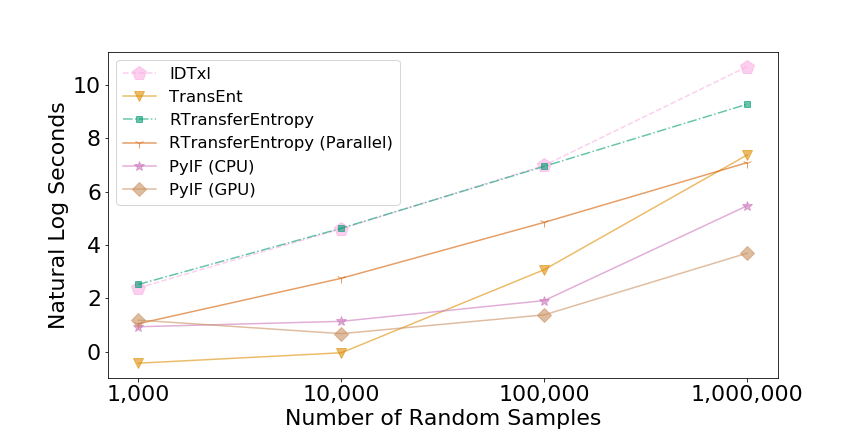
\includegraphics[scale=0.8]{figures/PyIF/WallTime-TE.png}}
  \caption{This figure shows the natural log time (in seconds) to estimate Transfer Entropy for each implementation (excluding Transfer Entropy Toolbox) for each dataset used in this study. }
  \label{TE-walltime}
\end{sidewaysfigure}


\begin{sidewaysfigure}[htb!]
  \centerline{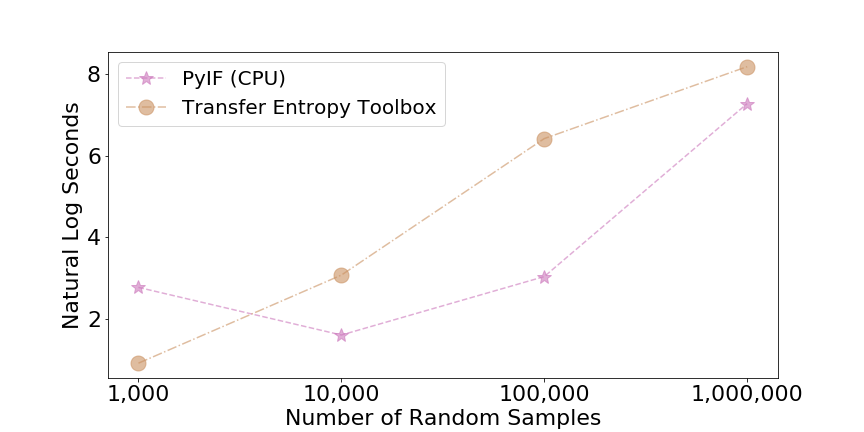
\includegraphics[scale=0.8]{figures/PyIF/WallTime-TE2.png}}
  \caption{This figure shows the natural log time (in seconds) to estimate Transfer Entropy between PyIF and Transfer Entropy Toolbox on an Engineering Workstation described in the Comparative Analysis section. Transfer Entropy Toolbox exceeded the maximum allowable CPU runtime for the Large Dataset. (1,000,000 observations). }
  \label{TE-walltime2}
\end{sidewaysfigure}

\clearpage

%\section*{Tables}

\begin{table}[htb!]
\centering
\resizebox{\columnwidth}{!}{
\begin{tabular}{|c|c|c|}
\hline
\textbf{Implementation}     & \textbf{Wall Time (in seconds)} & \textbf{Relative Performance to PyIF (CPU)} \\ \hline
IDTxl                       & 10.98                           & 4.28                                        \\ \hline
TransEnt                    & 0.656                           & 0.25                                        \\ \hline
RTransferEntropy            & 12.492                          & 4.87                                        \\ \hline
RTransferEntropy (Parallel) & 2.876                           & 1.12                                        \\ \hline
PyIF (CPU)                  & 2.564                           & 1                                           \\ \hline
PyIF (GPU)                  & 3.282                           & 1.28                \\ \hline                       
\end{tabular}
}
\caption{Micro Data results for the first analysis.}
\label{tab:MicroResults1}
\end{table}

\begin{table}[htb!]
\centering
\resizebox{\columnwidth}{!}{
\begin{tabular}{|c|c|c|} 
\hline
\textbf{Implementation}     & \textbf{Wall Time (in seconds)} & \textbf{Relative Performance to PyIF (CPU)} \\ \hline
IDTxl                       & 100.23                          & 31.94                                       \\ \hline
TransEnt                    & 0.968                           & 0.308                                       \\ \hline
RTransferEntropy            & 102.228                         & 32.57                                       \\ \hline
RTransferEntropy (Parallel) & 15.703                          & 5                                           \\ \hline
PyIF (CPU)                  & 3.138                           & 1                                           \\ \hline
PyIF (GPU)                  & 1.98                            & 0.63                                       \\ \hline
\end{tabular}
}
\caption{Small Data results for the first analysis.}
\label{tab:SmallResults1}
\end{table}

\begin{table}[htb!]
\centering
\resizebox{\columnwidth}{!}{
\begin{tabular}{|c|c|c|}
\hline
\textbf{Implementation}     & \textbf{Wall Time (in seconds)} & \textbf{Relative Performance to PyIF (CPU)} \\
IDTxl                       & 1070.749                        & 152.89                                      \\ \hline
TransEnt                    & 21.708                          & 3.03                                        \\ \hline
RTransferEntropy            & 1036.661                        & 152                                         \\ \hline
RTransferEntropy (Parallel) & 127.281                         & 18.66                                       \\ \hline
PyIF (CPU)                  & 6.82                            & 1                                           \\ \hline
PyIF (GPU)                  & 3.996                           & 0.58                      \\ \hline                 
\end{tabular}
}
\caption{Medium Data results for the first analysis.}
\label{tab:MediumResults1}
\end{table}

\begin{table}[htb!]
\centering
\resizebox{\columnwidth}{!}{
\begin{tabular}{|c|c|c|}
\hline
\textbf{Implementation}     & \textbf{Wall Time (in seconds)} & \textbf{Relative Performance to PyIF (CPU)} \\ \hline
IDTxl                       & 43150.129                       & 181.97                                      \\ \hline
TransEnt                    & 1585.942                        & 6.68                                        \\ \hline
RTransferEntropy            & 10592.77                        & 44.67                                       \\ \hline
RTransferEntropy (Parallel) & 1188.636                        & 5.01                                        \\ \hline
PyIF (CPU)                  & 237.122                         & 1                                           \\ \hline
PyIF (GPU)                  & 40.231                          & 0.16                                    \\ \hline   
\end{tabular}
}
\caption{Large Data results for the first analysis.}
\label{tab:LargeResults1}
\end{table}



% ake seperate table
\begin{table}[htb!]
\centering
\resizebox{\columnwidth}{!}{
		\begin{tabular}{ |c|c|c|  }
			\hline
			Implementation & Wall Time (in seconds) &  Relative Performance to PyIF (CPU) \\
 			\hline
			 \multicolumn{3}{|c|}{Micro Dataset Results (1000 Obs.)} \\
 			\hline
 			PyIF (CPU)   & 16.049 & 1.00\\ \hline
 			Transfer Entropy Toolbox & 2.5012 & 0.15 \\ \hline
 			\multicolumn{3}{|c|}{Small Dataset Results (10,000 Obs.)} \\
 			PyIF (CPU)   & 4.989 & 1.00\\ \hline
			 Transfer Entropy Toolbox & 21.6880 & 4.347 \\ \hline
 			\multicolumn{3}{|c|}{Medium Dataset Results (100,000 Obs.)} \\
 			\hline
 			PyIF (CPU)   & 20.915 & 1.00\\ \hline
			Transfer Entropy Toolbox & 616.8712 & 29.49 \\ \hline
 			\multicolumn{3}{|c|}{Large Dataset Results (1,00,000 Obs.)} \\
 			\hline
 			PyIF (CPU)   & 1455.725 & 1.00\\ \hline
			 Transfer Entropy Toolbox & $>$ 3600 & $>$ 2.47\\ 
			 \hline
			 

		\end{tabular}
	}
		\caption{Results for the second analysis.}
		%\caption{The wall time and relative performance to PyIF (CPU) to estimate Transfer Entropy between PyIF and Transfer Entropy Toolbox on an Engineering Workstation machine as described in the section Comparative Analysis.}
	\label{DataTable-MATLAB}
	
\end{table}

%\clearpage
\bibliographystyle{plainnat}
\nobibliography{thesisbib}
\chapter{Cross-Firm Information Transfers During Earnings Season: A Network Approach} \label{Chapter:EATE}
\blfootnote{
	This chapter contains material from the following working paper:  Robert Brunner, Kelechi Ikegwu, Bryce Schonberger, and Jeff McMullin. Cross-firm information transfers during earnings season: A network approach, April 2021 
	
	%\nobibliography{thesisbib}
	%\begin{itemize}
	%	\item\bibentry{EA-TE}
	%\end{itemize}
}

\section{Introduction}


Major public-firms announce their annual earnings during the first quarter of the year.  The information embedded in these announcements affects the share price of the announcing firm and is incorporated in the share prices of other firms.  Existing literature in finance and accounting focuses on measuring information transfers as effects stemming from firm-specific information releases, such as earnings announcements (see \cite{Foster1981}). This chapter explores how firm information releases influence other firms in the economy without prior assumptions.   We make two simplifying decisions when testing for informational links: an ex-ante source of fundamental linkage between firms, and a time window over which an information transfer will occur.  On the first point, most previous studies assume that links between firms are both persistent and readily observable by a characteristic such as a shared industry (see \cite{Foster1981}) or a customer-supplier relationship (see \cite{OlsenDietrich1985,  AhernHarford2014}).  On the second point, most studies examine an event window, typically several days long, around specific firms' announcements, such as announcing firms in an industry (see \cite{Foster1981, ThomasZhang2008}).

Research by \cite{Billio2012} uses a network approach to examine cross-firm transfers implicit in monthly equity returns for large firms in the financial services sector.  Consistent with a dynamic network of links among these financial firms, these authors find that the extent of cross-firm information transfers increases in recent decades and is associated with significant systemic risk in the financial sector, particularly around the recent 2007-2009 Great Recession.  Evidence presented by \cite{Billio2012} raises the natural question of whether dynamic cross-firm information transfers are present in a broad-based sample of firms and what factors explain variation within this network.

We construct a novel network approach during Q1 2018,  where the network relies on pairwise TE estimates between firms as a proxy for information transfer. Our approach contributes to extant accounting and finance literature.  We provide novel evidence on the network of cross-firm links implied by the lead-lag structure implicit in high-frequency U.S. equity prices observed around releases of earnings information.  By tracing the network of information transfers directly,  we can document several features of cross-firm links that go beyond industry or customer/supplier relationships.  Finally,  we use a community detection algorithm to uncover latent clusters of firms with shared information links.  Ultimately we provide evidence that the presence and size of these communities significantly differ depending on the presence of earnings releases.  We hope to encourage future work designed to broaden our understanding of the complex system of information flows inherent in modern equity markets. 

For the remainder of this chapter,  we first discuss the datasets used in this study.   Next, we discuss the methodology for estimating cross-firm information transfers and discuss the network science used to create dynamic cross-firm information transfer networks. We also make observations about the structural properties of the networks.  Then, we conduct an analysis to determine the effect of earnings surprise on dynamic cross-firm information transfers, and we discuss the results of the analysis.  Finally we present an analysis involving community detection within the network of cross-firm  information transfers and conclude.

\section{Data}
The data in the study comes from Wharton Research Data Services (WRDS) (see \cite{WRDS}). We obtain security prices from the Trade and Quote (TAQ) dataset, which contains all trades and quotes that occurred at a sub-second level.  We use SAS code provided by \cite{HoldenJacobsen2014} to measure the national best bid/offer(NBBO) price. The price is updated as trades or quotes occur.  This means that the timing of the share price updated and depends on when these events occur.  %The NBBO prices are identified from the TAQ dataset and are sampled at particular rates. 

We obtain the NBBO price data for firms in the S\&P 500 in Q1 2018.  We construct ten datasets for each firm at different sampling rates. The sampling rates used in this study are: $1$ second,  $2$ seconds,  $3$ seconds,  $4$ seconds,  $5$ seconds, $10$ seconds,  $15$ seconds,  $30$ seconds,  $60$ seconds,  and $120$ seconds.  For example, at $1$ second sampling rate, there will be 60 NBBO price observations per minute for a particular firm.  CRSP and Compustat are used to obtain firm-specific information.  We also use the Institutional Brokers' Estimate System (IBES) to obtain earnings announcement dates and times as well as earnings surprise for firms in the S\&P 500 during Q1 2018.  Throughout the text, we describe how variables are used from IBES, CRSP, and Compustat. 

%Micro structure noise?
% HERE!
\section{Estimating Dynamic Information Transfer Between Firms}

We estimate the amount of information transfer between every unique pair of firms in the S\&P 500 during Q1 2018 (the first 61 days of 2018) by using TE.  To detect information transfer at the minute/sub-minute level between firms in the S\&P 500, we first obtain the NBBO prices from the TAQ data for all firms in the S\&P 500 in Q1 2018.  As described above,  we create ten datasets from the NBBO data for each date and firm.  We sample the NBBO price data with the following sampling rates: 1,  2,  3,  5,  6,  10,  15,  30,  60,  and 120 seconds. We select these sampling frequencies to allow for a sufficiently large sample of pricing observations in each time window to compute TE.  By sampling price at a wide range of frequencies we can determine at what speed the observed  information transfers peak.  

Next,  for each date,  firm, and sampling rate,  we estimate bi-variate TE  with the NBBO sampled price data using three 130 minute windows throughout the trading day. We use these three windows to determine if there are any consistent information flow patterns during the beginning (9:30am-11:40am), middle (11:40am-1:50pm), or end (1:50pm-4pm) of the trading day.  To summarize TE is estimated to a specific firm from each of the other firms in the S\&P 500 for that particular date,  sampling rate,  and window.  Given that there are 10 sampling rates,  3 windows,  61 days,  and 499 other firms, this amounts to 913,170 TE calculations per firm for Q1 2018 (or 456,585,000 TE calculations in total).  

Data from small sample rates will yield a high number of observations.  %Given that the existing open-source implementations were not suited to estimate bi-variate TE on big data (see Chapter \ref{Chapter:PyIF}) we utilize PyIF (see \cite{PyIF}). 
The 1-second sampling rate has the most observations and is the most costly to estimate TE.  For a particular trading day,   running TE computations with PyIF (see Chapter \ref{Chapter:PyIF}) on the HAL cluster at the National Center for Supercomputing Applications using a single NVIDIA V100 GPU to 1 firm from the other 499 firms for the three windows will take roughly 4 minutes.  For all 500 firms, this took about 2000 minutes.  For all days in Q1 2018, this took about 122,000 minutes (or about 85 days) at the 1-second sampling rate sequentially.  Subsequently, for the 2-second sampling rate, the data is reduced by half. Thus, the wall time was reduced by roughly half.   Given that we can run up to five jobs in parallel on HAL, 1-second TE estimates took 17 days to compute. 

% With PyIF computing TE estimates using the HAL cluster at the National Center for Supercomputing Applications using a single NVIDIA V100 GPU. 

\subsection{Algorithmic Process for Estimating Information Transfer Between firms}

In this section, we outline the algorithmic process to estimate information transfer between firms using the Q1 2018 data (see Algorithm \ref{alg:EstIF}).  In Algorithm \ref{alg:EstIF},  we create a dictionary to map combinations of dates and sampling rates with matrices of computed information transfers.  Given the dates of interest in line 2 and the sampling rates in line 3, we iterate through each date in line 4.  For a particular date, we iterate through each sampling rate in line 5.  For each unique combination of date and sampling rate, we select firms with observations in that date and sampling rate. Next, we create an empty matrix of size Firms\(_i\)\(^2\) by 3, and we use a counter variable to keep track of the observations in line 9. 

Next, we iterate through each firm in the set of firms\(_i\).  In Algorithm \ref{alg:EstIF} the trading day is split into three,  two hour and ten minute windows that represent the beginning (9:30am-11:40am),  middle (11:40am-1:50pm),  and end of the trading day (1:50pm-4pm).  In lines 10-12, we filter the NBBO prices for firm i to the beginning of the trading day,  middle of the trading day, and end of the trading day for a single firm from the set of firms\(_i\) . We repeat this process for all of the firms in the set firms\(_j\) and estimate TE from firm\(_j\) to firm\(_i\).   The TE estimate is assigned to row cnt\(_{ij}\) and column zero of the dateSR\_InfoFlow matrix for the particular key of the dictionary for the TE computation with the morning prices.  Subsequently, the TE estimate is assigned to row cnt\(_{ij}\) and column one or two for the middle of the trading day or end of the trading day, respectively.   Finally, we increment cnt\(_{ij}\) by one and repeat this process for all pair of firms, sampling rates, and days.  Following this algorithm produces a dictionary of computed TEs, our proxy for information transfers,  for each unique pair of date and sampling rate. We perform our  analyses on this data.  \\

\begin{algorithm}[H]
\setstretch{1.45}

\SetAlgoLined
%\KwResult{Write here the result }

dateSR\_InfoFlow := \{ \} \;
Dates := All Dates in Q1 2018 \;
SampleRates := [1, 2, 3, 4,  6, 10, 30, 60, 120] secs \;

\For{\(t \in \) Dates}{
	\For{\(SR \in \) SampleRates}{
		Firms\(_i \) := SelectFirms(\(t,SR\)) \;
		Firms\(_j \) := SelectFirms(\(t,SR\)) \;
		dateSR\_InfoFlow[(t,SR)] := Matrix(length(Firms\(_i\))\(^2\), 3) \;
		cnt\(_{ij}\): = 0 \;
		\For{Firm\(_i \in\) Firms\(_i\)}{
			MoPrices\(_i\) := Filter(Firm\(_i\), “9:30am-11:40am”) \;
			MidPrices\(_i\) := Filter(Firm\(_i\), “11:40am-1:50pm”) \;
			AfterPrices\(_i\) := Filter(Firm\(_i\), “1:50pm-4:00pm”) \;	
						
			\For{Firm\(_j \in\) Firms\(_j\)}{
				MoPrices\(_j\) := Filter(Firm\(_j\), “9:30am-11:40am”) \;
				MidPrices\(_j\) := Filter(Firm\(_j\), “11:40am-1:50pm”) \;
				AfterPrices\(_j\) := Filter(Firm\(_j\), “1:50pm-4:00pm”) \;
				
				dateSR\_InfoFlow[(t,SR)] [cnt\(_{ij}\),0] := ComputeTE(MoPrices\(_i\), MoPrices\(_j\)) \;
				dateSR\_InfoFlow[(t,SR)] [cnt\(_{ij}\),1] := ComputeTE(MidPrices\(_i\), MidPrices\(_j\)) \;
				dateSR\_InfoFlow[(t,SR)] [cnt\(_{ij}\),2] := ComputeTE(AfterPrices\(_i\), AfterPrices\(_j\)) \;
				
				cnt\(_{ij}\) += 1
			}
		}
	}
}

\caption{Estimating Information Transfers Between Firms}
\label{alg:EstIF}
\end{algorithm}


\subsection{Network Creation}

After we compute all bi-variate TE estimates, we conduct exploratory data analysis to find patterns or characteristics of the information transfer between firms to explore further.   We employ network analysis techniques (see Chapter \ref{sec:NetworkScience}) to create an information transfer network for all firms at date $t$, sampling rate $s$, and window $w$.  Figure \ref{fig:ExampleNetwork} shows a single network for January 2nd,  2018, during the morning window (9:30am-11:40am).  Each circle in the network is a node that represents a firm. The lines (or edges) between nodes have a thickness determined by the information transfer estimate as computed via transfer entropy. 

The information transfer network in Figure~\ref{fig:ExampleNetwork} has been filtered with a disparity filter (see \cite{Serrano}) to reduce the amount of edges in a network.  However, it is still challenging to gather insight from this network.  In addition, there is an information transfer network for each $t$,  $s$,  and $w$. Creating networks for all days,  sampling rates, and windows will produce roughly 1,830 networks, which will make it more difficult to discover general insights from the data by viewing them.  We take an alternative by examining at network measures to gain additional insights about the information transfer networks.

% For all 3 figures roughly 2000 edges are displayed, displaying the full 250,000 connections would yield a network where the ratio of firms to connections is too high to display in this display.  Nevertheless,  representing the data as a network offers an alternative strategy which allows us to compute common network metrics and explore the relationships between firms.

\section{Exploratory Data Analysis}

We now turn to an exploratory analysis of the computed information measures. Figure \ref{fig:TEDist} shows the distribution of information transfers for all days in Q1 2018 for all windows at each sampling rate.   Each subplot is for a particular sample rate,  the x-axis represents the bin value,  and the y-axis represents the percentage of observations in a bin.  Faster sampling rates have lower variance and higher means.  Slower sampling rates have higher variance and smaller means.  A possible explanation is that the frequency of observations decreases due to fewer non-overlapping observations during each 130-minute window.   For example,  there are 7,800 observations per firm at a 1-second sample rate and 130 observations per firm at a 1-minute sample rate. The 1-minute yields fewer data to compute TE and produces a noisier information transfer estimate. 

Table \ref{tab:TEDistIndSampleRate} show additional summary statistics of the information transfers at  each sampling rate.  The 75th and 99th percentile values increase while the median percentile (and lower) values decay as the sample rate becomes slower.  Table \ref{tab:TEMeanWindows} contains the average TE values computed for each of the 130-minute trading windows during the first quarter of 2018 for pairs of firms in the S\&P 500.  

Across sampling rates,  Table \ref{tab:TEMeanWindows} mean values exhibit similar patterns to Table \ref{tab:TEDistIndSampleRate} with a decrease in means as the sampling rates become slower.  Across the three 130-minute windows on each trading day, the 9:30 am-11:40 am (morning) window displays the highest average information transfer.  This latter result is consistent with a surge in trading at the market open each day.

In Table \ref{tab:TEMean30MinWindows},  we investigate the mean TE values at narrower time windows to determine when information transfers tend to peak during the trading day.  Table \ref{tab:TEMean30MinWindows} contains the average TE values computed for thirteen, non-overlapping, thirty-minute trading windows.  Across all sampling rates,  average TE values are highest during the first thirty minutes of the trading day.  Mean TE values then decay throughout the trading day at all sampling rates.  Sampling rates faster than 6 seconds have a slight burst of information transfer within the last hour of the trading day, consistent with information-based trading as part of the daily settlement (closing) trade. 


Table \ref{tab:TEMeanScaledWeightedOutDegree}} shows the average weighted out-degree of the information transfer network at various sampling rates across 61 morning trading periods (9:30am-11:40am).  We scale each degree measure by the number of firms in the network at each measurement period.  Since all firms in the information transfer networks are connected, the average weighted out-degree values across all firms in the first quarter of 2018 are equivalent to the mean weighted in-degree values.  Stated differently, the average of all incoming information transfers from a set of firms to a particular firm is equivalent to the average of all outgoing connections from a set of firms to a firm. The average weighted incoming and outgoing information transfer spikes at a sampling rate of 5 – 6 seconds.


%Given that the Kraskov estimator has a downward bias (see Chapter \ref{IFinFM}) some TE values are slightly below 0.  Figures \ref{fig:20180102-1sec-1of3},  \ref{fig:20180102-1sec-2of3},  and \ref{fig:20180102-1sec-3of3},  show examples of a reduced network on January 2nd 2018 at the 1 second sampling rate between 9:30am-11:40am, 11:40am-1:50pm, and 1:50pm-4pm respectively.   Each of these figures show a portion of the firms in the S\&P 500 and the connections between them, where the firms are the nodes and the connections are the edges with a thickness determined by the value of the transfer entropy estimate.  The highest 0.5\% of edges in the network at these particular times are displayed.  

Tables \ref{tab:TEAutoCorrIn} and \ref{tab:TEAutoCorrOut} present results of ordinary least squares models examining auto-correlation in daily measures of weighted network degree to determine whether firms’ centrality in the network of information transfers displays persistence.  In particular, Table \ref{tab:TEAutoCorrIn} (Table \ref{tab:TEAutoCorrOut}) presents auto-correlations for incoming (outgoing) information transfers based on the weighted in-degree (out-degree) computed from 9:30am-11:40am for each trading day in our 2018 sample period.  The $R^2$ values for both tables exhibit similar behaviors across sampling rates.  In particular, at faster sampling rates we see more explained variation from the morning information transfers with a gradual decay as the sample rates become slower.  The $R^2$ values for the auto-correlation models for outgoing information transfers during morning trading windows in Table \ref{tab:TEAutoCorrOut} are substantially higher than the incoming morning information transfers in Table \ref{tab:TEAutoCorrIn}.  This provides evidence that each firm's position in the information transfer network is persistent. 


\section{Earnings Surprise as a Determinant of Dynamic Information Transfers} % Section with Regression 


Prior literature finds that more informative news events elicit more robust stock price responses among peer firms (see \cite{Foster1981,  Brochet2018}).  Given this,  we examine whether firms with larger absolute earnings surprises (measured relative to the consensus analyst forecast) display stronger information transfers in response to their earnings announcement.  This analysis allows us to shed light on the dynamics of the information transfer network by focusing on variation in the timing of firm’s earnings announcements during earnings season and on variation in the news contained in the announcement.  

In particular,  we estimate an ordinary least squares regression model of the form:

\setlength{\arraycolsep}{0.0em}
\begin{eqnarray}
Y_{iwt} = \alpha + \beta_1 EA_{iwt}  * Morning_{iwt} + \beta_2 EA_{iwt}  * Morning_{iwt} * Abs\_Suprise_{iwt} + \nonumber\\
\beta_3 EA_{iwt}  * Afternoon_{iwt} + \beta_4 EA_{iwt}  * Afternoon_{iwt} * Abs\_Suprise_{iwt} + \nonumber\\
\beta_5 EA_{iwt}  * Evening_{iwt} + \beta_6 EA_{iwt}  * Evening_{iwt} * Abs\_Suprise_{iwt} + \nonumber\\
\beta_7 Share\_Turnover_{it} + \beta_8 Abs\_RET_{it} + \nonumber\\
\beta_9 Morning_{it} + \beta_{10} Evening_{it} + \eta_{i} + \lambda_t +  \epsilon_{i}
\label{eq:EA-Surprise}
\end{eqnarray}
\setlength{\arraycolsep}{1pt}

\noindent \(Y_{iwt}\) is the weighted out-degree (or in-degree) for the \(i^{th}\) firm at the day \(t\) and window \(w\) (i.e, morning, afternoon, or evening).    \(EA_{iwt}\) is an indicator variable for the \(i^{th}\) firm at day \(t\) and window \(w\)  which is set equal to one for trading days with an earnings announcement for the \(i^{th}\) firm made after the prior market close or during the current trading day and to zero otherwise.   \(Morning\),  \(Afternoon\),  and \(Evening\) are indicators variables set equal to one if the current observation is during the 9:30 am - 11:40 am, 11:40 am-1:50 pm,  and 1:50 pm-4:00 pm trading windows, respectively.   

\(Abs\_Surprise\) is the absolute value of the quarterly earnings surprise measured as the difference between actual earnings in I/B/E/S and the last available consensus analyst earnings forecast from the I/B/E/S Summary file,  scaled by the quarter-end stock price available from Compsutat.  As modeled above,  the \(Abs\_Surprise\) variable only enters the model for the first Morning, Afternoon, and Evening trading windows following the announcement.   \(Share\_Turnover\) controls for the number of shares traded during the trading day, scaled by the number of shares outstanding on CRSP.  \(Abs\_RET\) is the absolute value of the close-to-close stock return from CRSP for the trading day.  Equation \ref{eq:EA-Surprise} treats each 130-minute trading window for each firm as a distinct observation.   To focus on within-firm variation in centrality we include firm-fixed effects \(\eta_1\) and trading day fixed-effects \(\lambda_t\). This analysis excludes four outlying observations with absolute earnings surprises larger than 5\% of price. 

We present results of estimating Equation~\ref{eq:EA-Surprise} in Tables~\ref{tab:TEDetOutDeg} and \ref{tab:TEDetInDeg},  where Table \ref{tab:TEDetOutDeg} (Table \ref{tab:TEDetInDeg}) presents results of OLS models where weighted out-degree (in-degree) is the dependent variable.   Results in Table \ref{tab:TEDetOutDeg} show that a firm’s weighted out-degree in the network of information transfers is significantly higher in the trading periods immediately following its earnings announcement when the firm announces a larger earnings surprise. In particular, the positive coefficient on the \(EA*Morning*Abs\_Surprise\) term across the sample rates in models (1) – (10) ranges from 1.672 in model (1) for the 1-second sample rate to 3.117 in model (4) for the 5-second sample rate.  All estimates are statistically significant at a 5\% two-tailed level.  Further, the pattern in coefficients on the \(EA*Morning*Abs\_Surprise\) term across models (1) – (10) in Table \ref{tab:TEDetOutDeg} suggests an information transfer that peaks at 5 seconds, consistent with our transfer entropy estimates presented in Table \ref{tab:TEDistIndSampleRate}.  A significant relation between weighted\_out-degree and earnings news persists into the afternoon trading window at faster sample rates, with significant positive coefficients on the \(EA*Afternoon*Abs\_Surprise\) term for sample rates ranging from 1 second to 3 seconds in models (1) – (3) (two-tailed p-values < 0.05). 

Turning to results in Table \ref{tab:TEDetInDeg} for weighted network in-degree shows that in contrast to results in Table \ref{tab:TEDetOutDeg},  weighted\_in-degree displays limited variation with the magnitude of earnings news released. Except for the \(EA*Morning*Abs\_Surprise\) term in models (1) and (2) for the fastest sample rates, coefficients on the interaction terms with \(Abs\_Surprise\) are generally insignificant at conventional levels and display no clear pattern across sample rates. We interpret these results as suggesting that transfers out to other firms are significant in response to the magnitude of earnings news released, while transfers in are limited in response to the news released.

\section{Community Detection}

We attempt to use community detection algorithms on the information transfer networks to uncover dynamic community formation across morning trading windows.  To limit computational time, we select three morning trading periods for analysis: two periods with a large number of earnings announcements (January 31 and February 1) and one period with no earnings announcements (March 13). We further focus on information transfers at faster speeds by taking the average information transfer across 1 – 6 second sampling rates for each of the three morning trading windows selected and reconstruct the information transfer network.  

In network science literature,  a standard definition of a community is having more nodes grouped where there is a higher density of edges within the group than between groups.  Given that the information transfer networks are relatively large, we utilize the Clauset-Newman-Moore greedy modularity maximization algorithm to find communities \citep[see][]{Clauset2005}.  While the Clauset-Newman-Moore algorithm aims to find communities in vast networks, it cannot find communities in the information transfer networks. 

The density in our information transfer networks are \(1\), whereas \cite{Clauset2005} benchmark network had a density of \(0.0000125\). Another way to think of this is that the ratio of edges to nodes in our network is 100 times greater than their benchmark network.  While we would ideally employ a community detection algorithm able to scale to the size of these information transfer networks, we are unaware of an such an algorithm.  Thus, we take an alternative approach by reducing the nodes-to-edges ratios for our information transfer networks. This allows us to use standard community detection algorithms.  


To use the Clauset-Newman-Moore algorithm, we combat the density issue by reducing the density (or the node to edges ratio).  \cite{Serrano} introduced the concept of disparity filters for weighted networks.  In this paper, they outline the algorithm to apply a disparity filter to networks.  \cite{Serrano} measures the strength of a node \(i\) as:

\begin{equation}
s_i = \sum_j w_{ij}.
\end{equation}

\noindent \(w_{ij}\) is the weight of the edge or transfer entropy value in the information transfer networks.  Each of the outgoing edges is scaled by \(s_i\): 

\begin{equation}
p_{ij} = \frac{w_{ij}}{s_i}.
\end{equation}

\noindent The disparity filter algorithm is based on the p-value statistical significance test of the null model of an information transfer network. \cite{Serrano} shows that the null model for a given network with a node of degree \(k\) is:

\begin{equation}
\alpha_{ij} = (1 - p_{ij})^{k-1}
\end{equation}

\noindent Meaning that \(\alpha_{ij}\) is the probability of having a normalized weight larger or equal to \(p_{ij}\) in the null model.  Selecting an \(\alpha\) will filter out all \(\alpha_{ij}\)'s larger than it resulting in the "network backbone" that contains significant edges between nodes.

We apply a disparity filter (see \cite{Serrano}) to three information transfer networks to identify the network backbone.  Stated differently,  the disparity filter locally identifies statistically relevant weighted edges and can filter out relevant connections across all scales of interactions between firms.  Specifically, this method removes any edge that is weaker than a statistical cutoff designed to measure the importance of a given connection to each node.  As a result, the key input for the disparity filter is a researcher-selected value for \(\alpha \) used to identify sufficiently strong connections between nodes. 

Our procedure is as follows. We first take the average information transfer across 1 – 6 second sampling rates for the morning trading windows for the three dates and reconstruct the information transfer networks.  Next, we apply the disparity filter to find the network backbone, which requires a value for \(\alpha\). The selection of \(\alpha\) requires fine tuning.  Table \ref{tab:backBoneSizes} shows the amount of nodes and edges remaining in a filtered network at a particular  \(\alpha\) value.  A smaller \(\alpha\) will yield an information transfer network that is too sparse to detect communities. A large \(\alpha\) will yield an information transfer network that is too dense to detect communities. 

We select \(\alpha\) based on the Clauset-Newman-Moore algorithm’s ability to detect communities for the most firms in the sample information transfer networks.  We found that when \(\alpha\) = 0.375,  we can detect communities for 100\% of the firms on February 1st and 97\% of the firms on January 31st and March 13th.  We find fewer communities formed during announcement days (January 31st and February 1st) than the trading day with no announcements (March 13th).  However,  most of the community’s sizes during the announcement days are larger than the communities in the March 13th information transfer network (see Figure \ref{fig:NetworkBackboneCommunitySizes}).  On this point,  Figure \ref{fig:NetworkBackboneCommunitySizes} shows that most of the firms in the March 13th information transfer network are in communities with 1, 2, or 3 other firms. During the announcement days, it is less likely to see communities with 1, 2, or 3 other firms; instead, we find more communities with larger sizes.

On the two days with many earnings announcements,  the communities typically have only one firm that announced.  There are three cases where a community has two firms that announced and one case where three firms announced. We see a diverse set of industries connected within and across the detected communities.   Figure \ref{fig:Community20180313full} presents the full set of nodes and resulting communities for the information transfer network for the March 13th morning trading window. This figure shows the presence of several larger communities with a handful of central (larger) nodes. In addition, Figure \ref{fig:Community20180313full} shows a number of firms (in gray) appearing with small (or no) communities.   To aid in graphically presenting these communities, Figures \ref{fig:Community20180131},  \ref{fig:Community20180201}, and \ref{fig:Community20180313}  presents only communities with at least 9 firms in the resulting community.  

For all the information transfer networks, there is a dynamic formation of hubs.  Some hubs reoccur, and others form during a particular trading day.   For example,  in Figures \ref{fig:Community20180131},  \ref{fig:Community20180201}, and \ref{fig:Community20180313} Amazon (AMZN), News Corp (NWS), and Mettler-Toledo International Inc (MTD) are hubs during the announcement days and the non-announcement day despite the different connections that form to each of these hubs.  However, when Boeing (BA) announced on January 31st, it temporarily appears as a hub in Figure~\ref{fig:Community20180131} for that morning information transfer network. The networks' characteristics provide evidence that the networks are not random, which provides evidence that we capture valid cross-firm information transfers via our measurement of transfer entropies. 
 

\section{Conclusion}

We introduce a new approach to examine information transfers around earnings season.  We study the network effect of earnings announcements by constructing daily networks of pairwise cross-firm information transfers.  Our approach to construct these networks relies on non-parametric estimates in equity prices with measures of transfer entropy drawn from information theory.  While it is known that earnings information produced by a single firm is incorporated into the firm's equity price,  we provide evidence that this information flows to the equity prices of other firms across industries.  In particular our tests show that cross-firm links are substantially stronger for firms on days with releases of earnings information and firms with more unexpected earnings news, consistent with the network of cross-firm information transfers dynamically responding to shifts in the information landscape.  Further,  we find that communities form between firms with links that are not adequately captured by characteristics that are the focus of existing literature.  These analyses also demonstrate that the prior literature’s focus on measuring information connections between firms in the same industry or along the supply chain likely result in missing important information linkages across more diverse firms. 


%Future work?

%Communtity detection algorithm for denser network


\newpage
\section{Figures and Tables}
%\subsection{Figures}

\rotatebox{90}{\begin{minipage}{0.9\textheight}
   \centerline{ 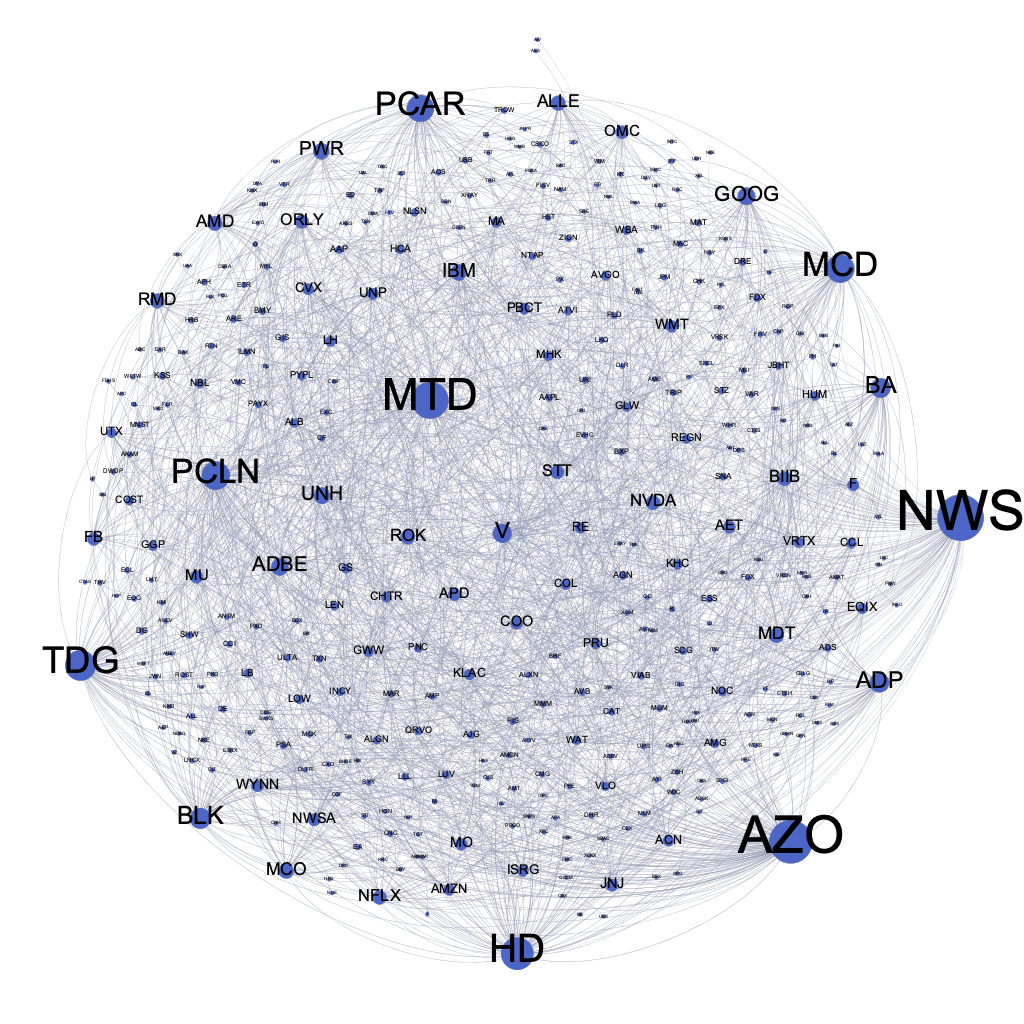
\includegraphics[width=0.7\textwidth]{figures/EarnAnnounceTE/ExampleNetwork-Jan2nd.png}}
    \captionof{figure}{This figure shows an example network on January 2nd during the morning window (9:30 am-11:40 am) at the 1-second sampling rate.}
  \label{fig:ExampleNetwork}
\end{minipage}}



%\begin{figure}[htb!]
%  \centerline{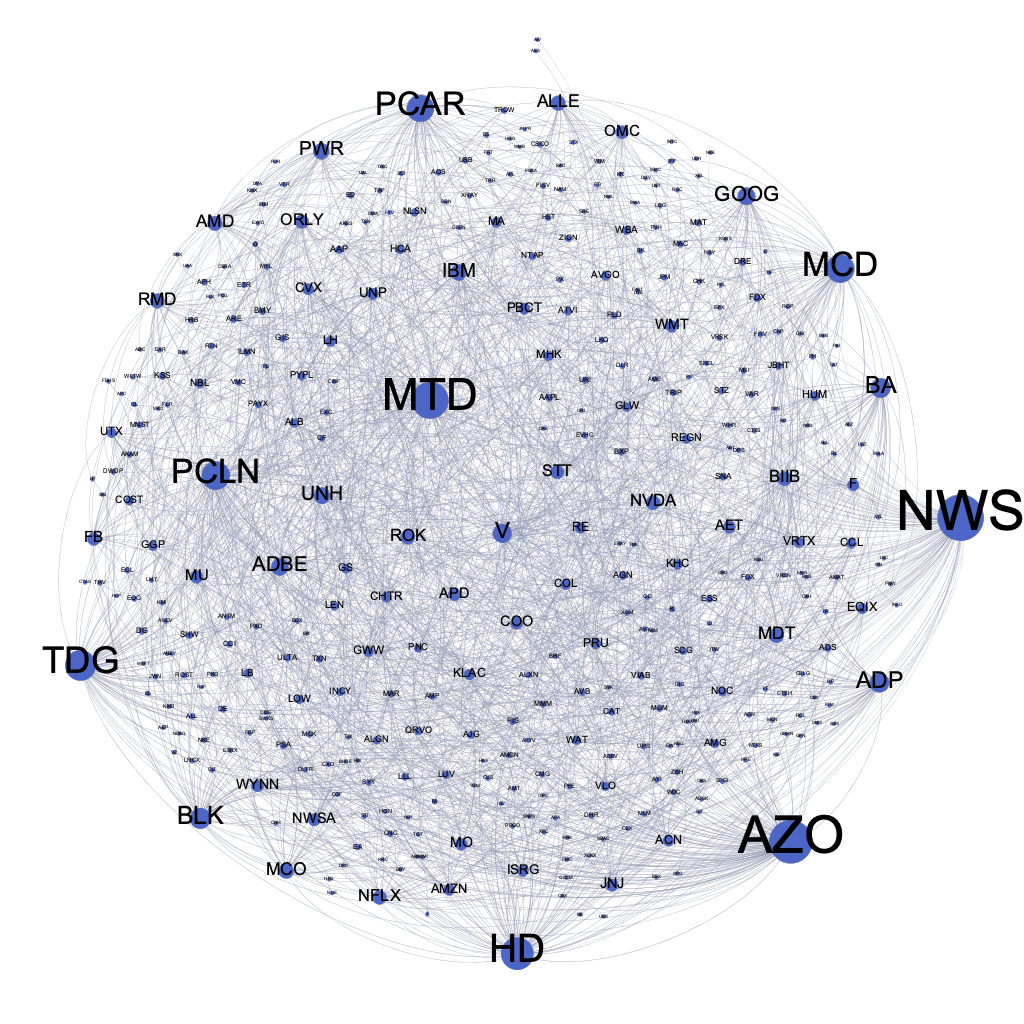
\includegraphics[scale=0.45]{figures/EarnAnnounceTE/ExampleNetwork-Jan2nd.png}}
%  \caption{This figure shows an example network on January 2nd during the morning window (9:30 am-11:40 am) at the 1-second sampling rate.}
%  \label{fig:ExampleNetwork}
%\end{figure}

\begin{figure}[htb!]
  \centerline{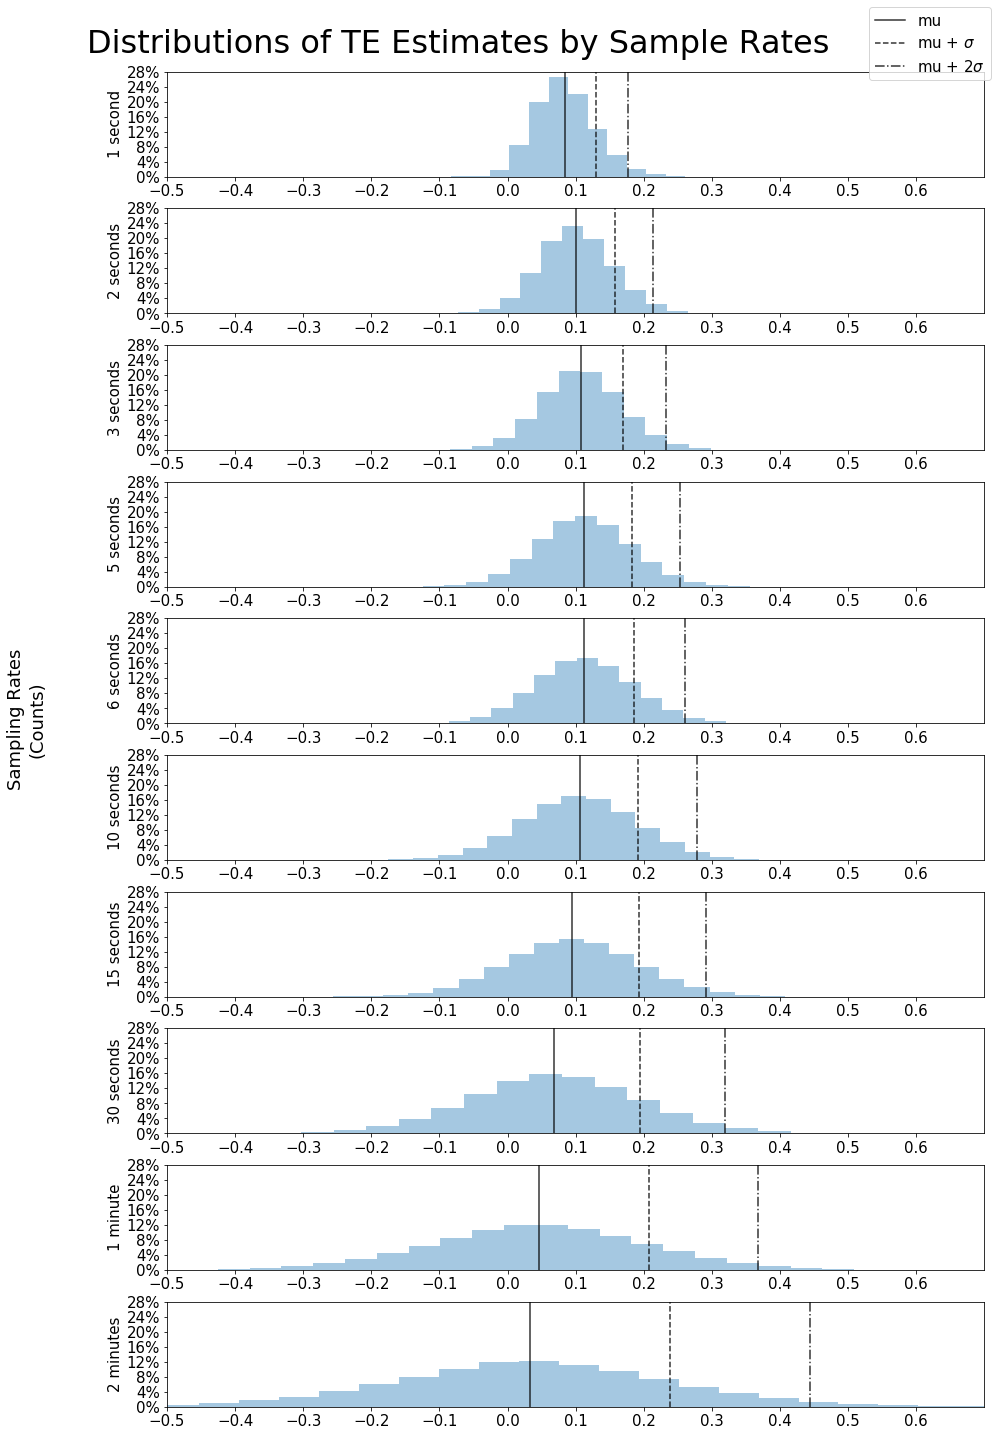
\includegraphics[scale=0.4]{figures/EarnAnnounceTE/TEDist.png}}
  \caption{This figure shows the distributions of information transfers between firms during Q1 2018 for all sampling rates.}
  \label{fig:TEDist}
\end{figure}

\begin{sidewaysfigure}[htb!]
  \centerline{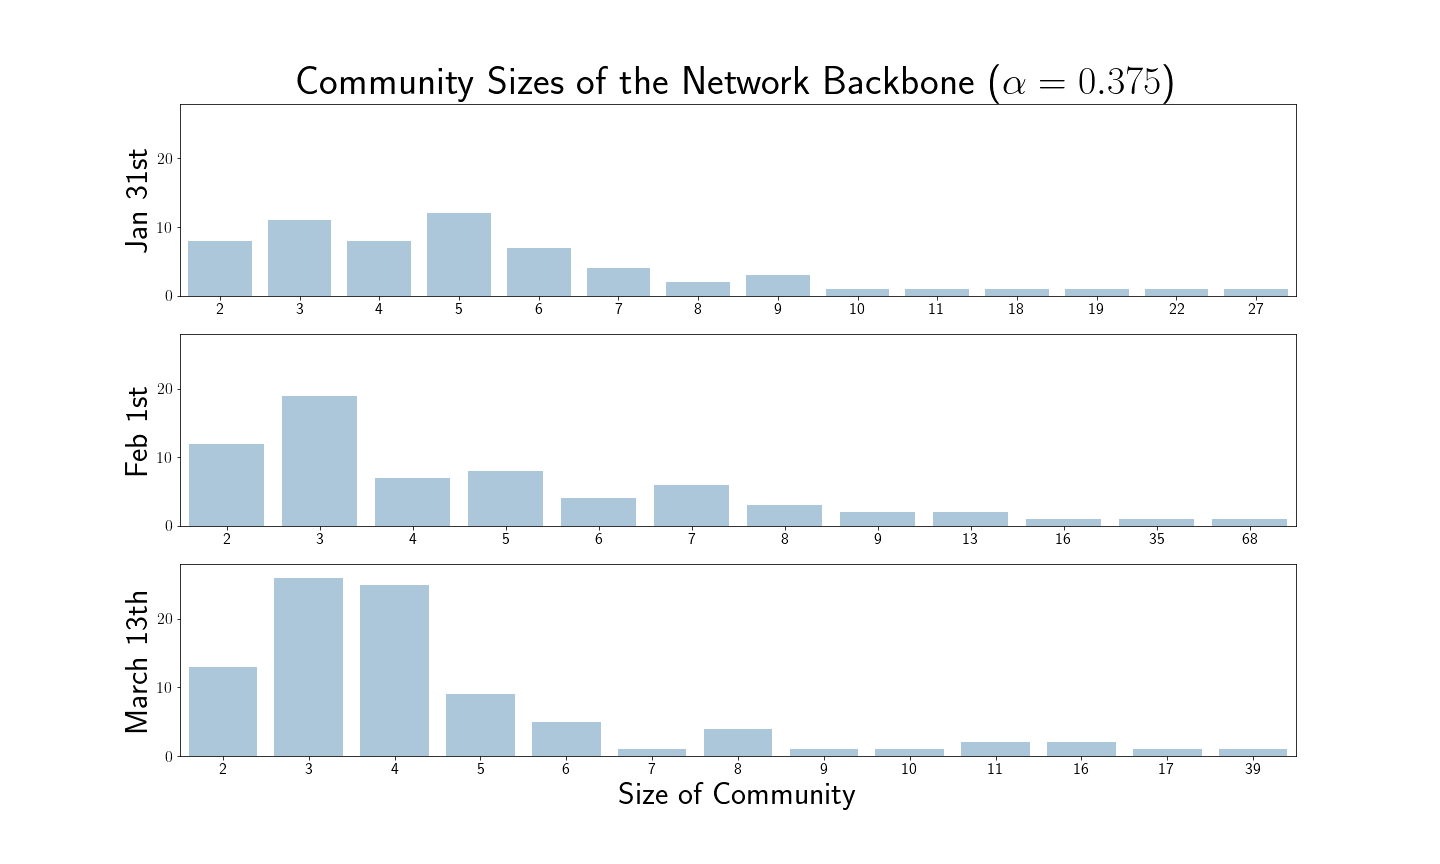
\includegraphics[scale=0.4]{figures/EarnAnnounceTE/NetworkBackboneCommunitySizes.png}}
  \caption{Community sizes of the network backbone when $\alpha=0.375$ for January 31st,  February 1st,  and March 13th}
  \label{fig:NetworkBackboneCommunitySizes}
\end{sidewaysfigure}

% Communtity Detection

\begin{figure}[htb!]
  \centerline{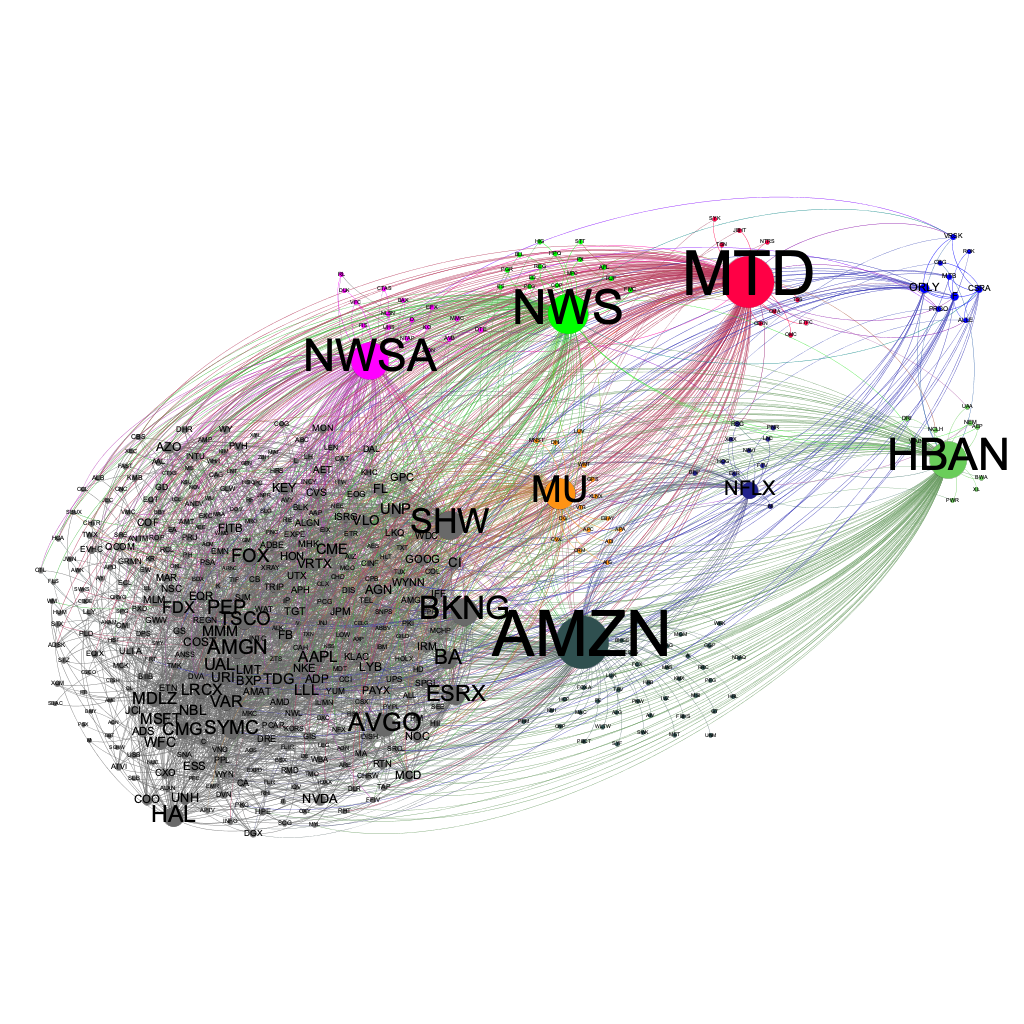
\includegraphics[scale=0.5]{figures/EarnAnnounceTE/20180313mt-8colored-curved}}
  \caption{This figure shows the backbone network displaying communities for March 13th.  Each color represents a specific community, and the node's size represents the degree of the node.  All communities and nodes with at least 9 firms appear with a color other than gray for each community. }
  \label{fig:Community20180313full}
\end{figure}


\begin{figure}[htb!]
  \centerline{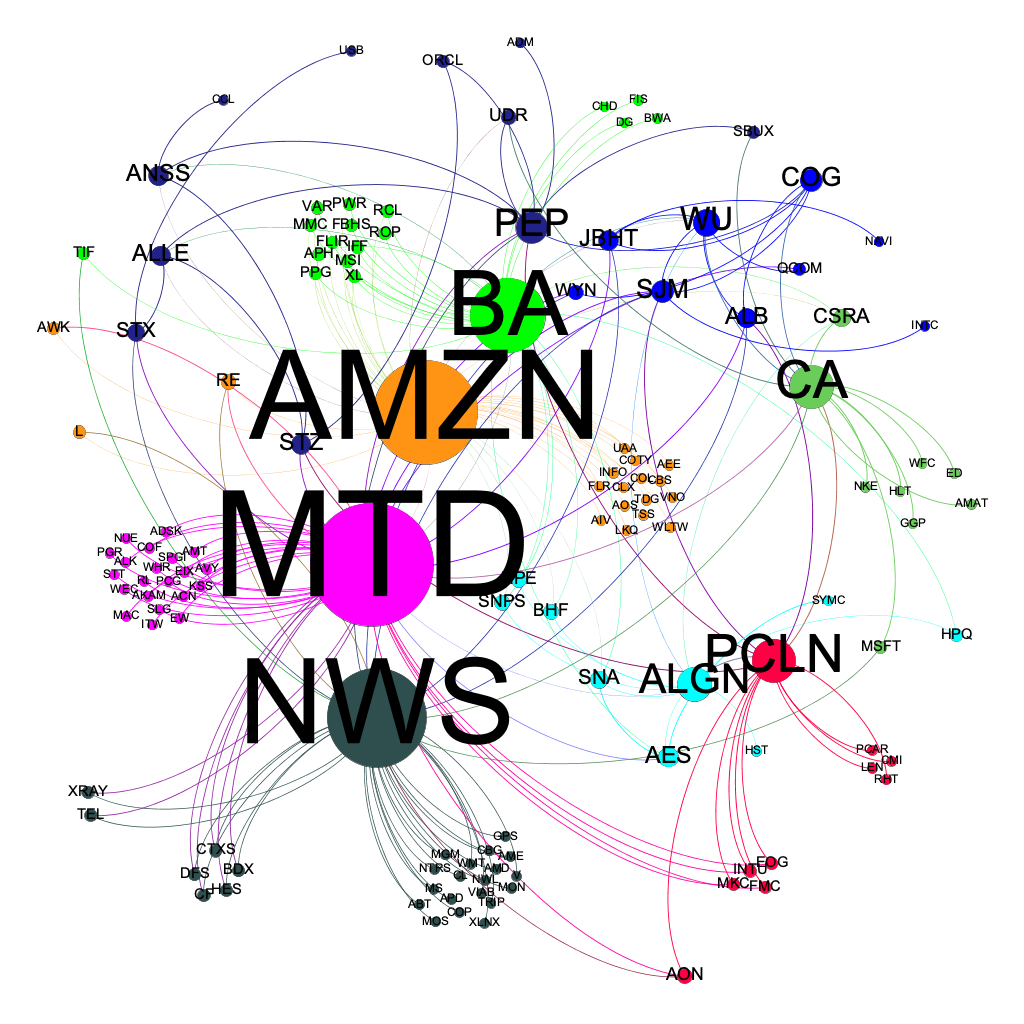
\includegraphics[scale=0.5]{figures/EarnAnnounceTE/20180131OnlyC-curved.png}}
  \caption{This figure shows the backbone network displaying communities for January 31st, where at least nine firms are in the community.  Each color represents a specific community, and the node's size represents the degree of the node.}
  \label{fig:Community20180131}
\end{figure}

\begin{figure}[htb!]
  \centerline{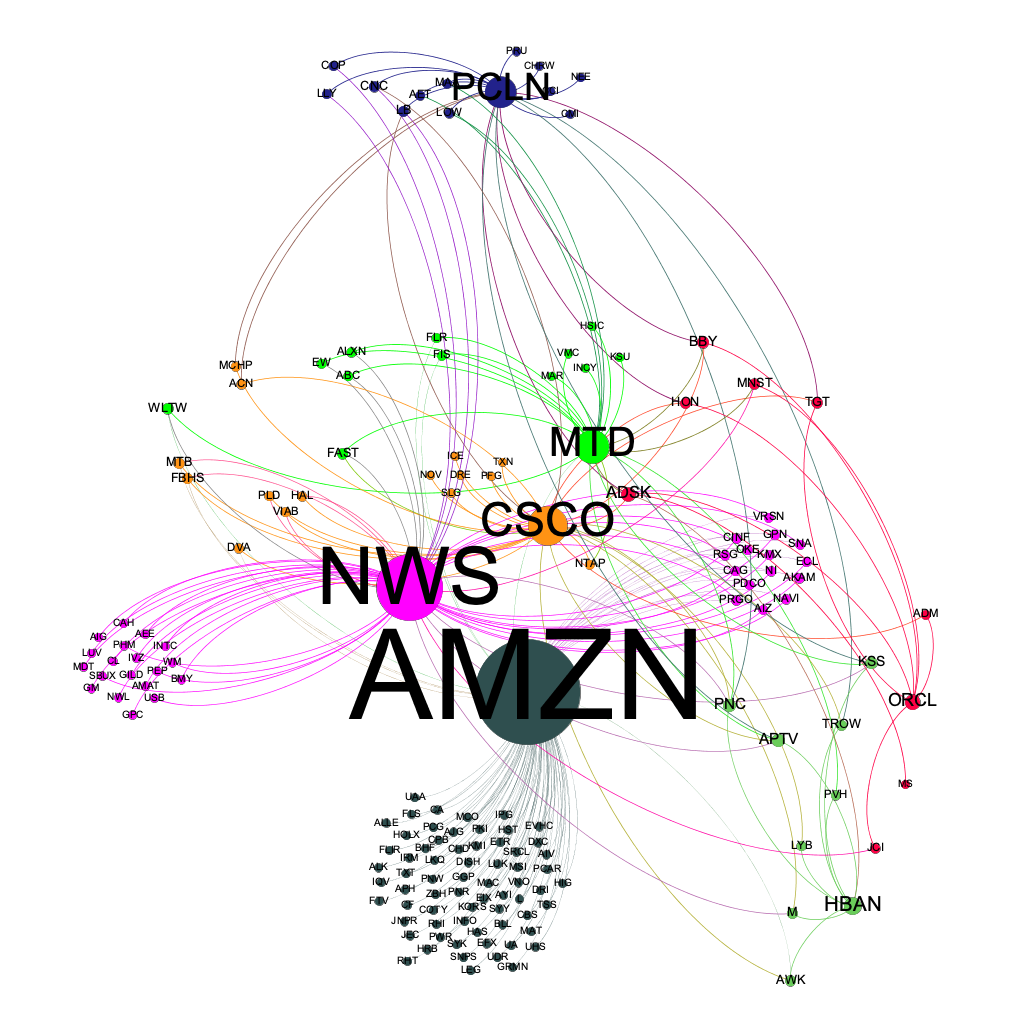
\includegraphics[scale=0.5]{figures/EarnAnnounceTE/20180201OnlyC-curved.png}}
  \caption{This figure shows the backbone network displaying communities for February 1st, where at least nine firms are in the community.  Each color represents a specific community, and the node's size represents the degree of the node.}
  \label{fig:Community20180201}
\end{figure}

\begin{figure}[htb!]
  \centerline{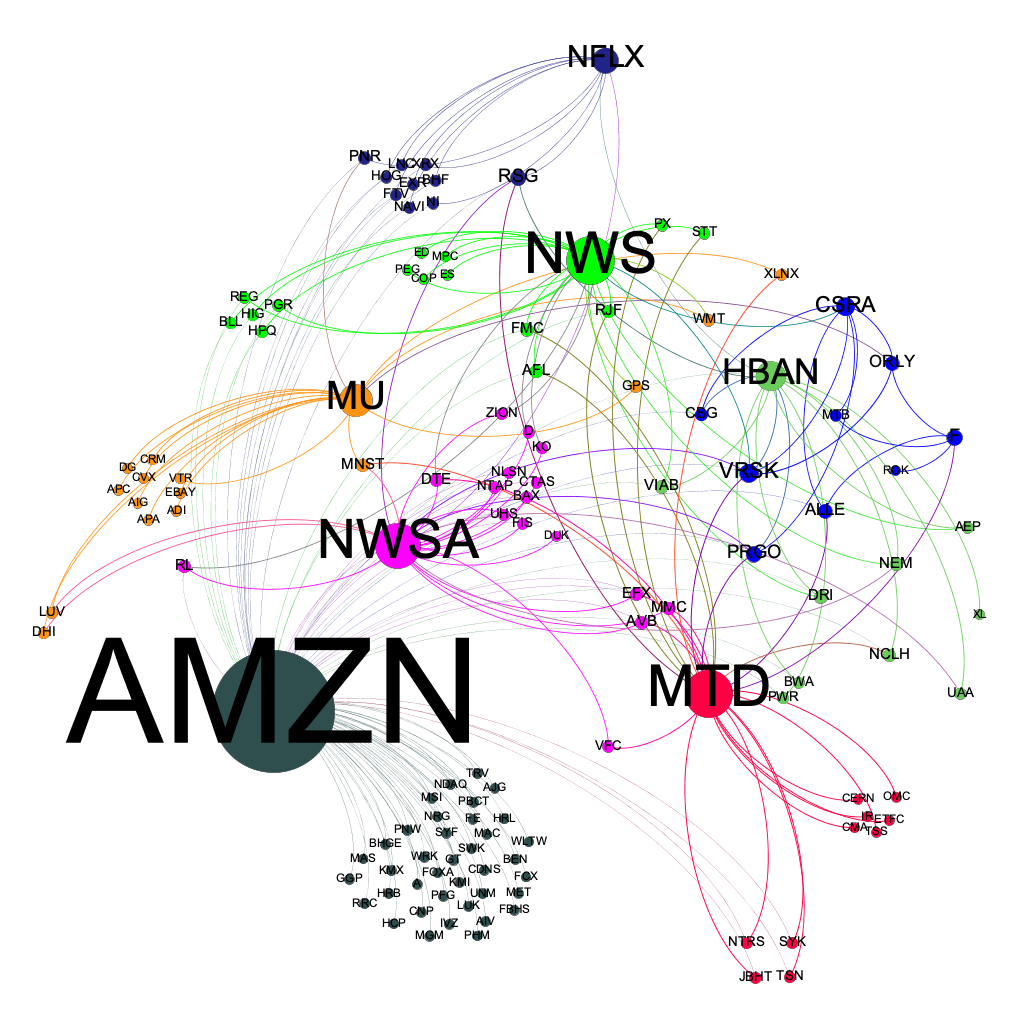
\includegraphics[scale=0.5]{figures/EarnAnnounceTE/20180313OnlyC-curved.png}}
  \caption{This figure shows the backbone network displaying communities for March 13th where at least nine firms are in the community.  Each color represents a specific community, and the node's size represents the degree of the node.}
  \label{fig:Community20180313}
\end{figure}



\clearpage

\begin{sidewaystable*}[htb!]
\centering
\resizebox{\columnwidth}{!}{
\begin{tabular}{|l|c|c|c|c|c|c|c|c|c|c|}
\hline
\multicolumn{1}{|r|}{\textbf{Sample Rate}} & \textbf{1 second} & \textbf{2 seconds} & \textbf{3 seconds} & \textbf{5 seconds} & \textbf{6 seconds} & \textbf{10 seconds} & \textbf{15 seconds} & \textbf{30 seconds} & \textbf{1 minute} & \textbf{2 minutes} \\ \hline
\textbf{Mean}                              & 0.084             & 0.101              & 0.108              & 0.112              & 0.112              & 0.106               & 0.094               & 0.069               & 0.046             & 0.033              \\ \hline
\textbf{St. Deviation}                     & 0.046             & 0.056              & 0.062              & 0.070              & 0.074              & 0.086               & 0.099               & 0.125               & 0.161             & 0.206              \\ \hline
\textbf{1st percentile}                    & -0.014            & -0.025             & -0.033             & -0.052             & -0.061             & -0.099              & -0.141              & -0.233              & -0.344            & -0.472             \\ \hline
\textbf{Q1}                                & 0.054             & 0.065              & 0.069              & 0.067              & 0.064              & 0.049               & 0.030               & -0.013              & -0.058            & -0.098             \\ \hline
\textbf{Median}                            & 0.082             & 0.100              & 0.108              & 0.112              & 0.112              & 0.106               & 0.094               & 0.069               & 0.047             & 0.034              \\ \hline
\textbf{Q3}                                & 0.112             & 0.136              & 0.148              & 0.158              & 0.160              & 0.163               & 0.159               & 0.152               & 0.153             & 0.167              \\ \hline
\textbf{99th percentile}                   & 0.201             & 0.234              & 0.253              & 0.275              & 0.283              & 0.306               & 0.323               & 0.359               & 0.422             & 0.517              \\ \hline
\end{tabular}
}
\caption{This table shows the summary statistics for transfer entropy estimates during non-overlapping 130-minute trading windows. }
\label{tab:TEDistIndSampleRate}
\end{sidewaystable*}


\begin{sidewaystable*}[htb!]
\centering
\resizebox{\columnwidth}{!}{
\begin{tabular}{|c|c|c|c|c|c|c|c|c|c|c|}
\hline
\multicolumn{1}{|r|}{\textbf{Sample Rate}} & \textbf{1 second} & \textbf{2 seconds} & \textbf{3 seconds} & \textbf{5 seconds} & \textbf{6 seconds} & \textbf{10 seconds} & \textbf{15 seconds} & \textbf{30 seconds} & \textbf{1 minute} & \textbf{2 minutes} \\ \hline
\textbf{9:30am-11:40am}                    & 0.097             & 0.117              & 0.125              & 0.130              & 0.130              & 0.123               & 0.109               & 0.082               & 0.058             & 0.044              \\ \hline
\textbf{11:40am-1:50pm}                    & 0.071             & 0.088              & 0.096              & 0.102              & 0.103              & 0.100               & 0.091               & 0.067               & 0.044             & 0.030              \\ \hline
\textbf{1:50pm-4pm}                        & 0.083             & 0.098              & 0.103              & 0.105              & 0.103              & 0.095               & 0.082               & 0.057               & 0.037             & 0.024              \\ \hline
\end{tabular}
}
\caption{Mean transfer entropy estimates for non-overlapping 130-minute daily trading windows at each sample rate.}
\label{tab:TEMeanWindows}
\end{sidewaystable*}

\begin{sidewaystable*}[htb!]
\centering
\resizebox{\columnwidth}{!}{
\begin{tabular}{|c|c|c|c|c|c|c|c|c|}
\hline
\multicolumn{1}{|r|}{\textbf{Sample Rate}} & \textbf{1 second} & \textbf{2 seconds} & \textbf{3 seconds} & \textbf{5 seconds} & \textbf{6 seconds} & \textbf{10 seconds} & \textbf{15 seconds} & \textbf{30 seconds} \\ \hline
\textbf{09:30AM-10:00AM}                   & 0.099             & 0.118              & 0.127              & 0.130              & 0.129              & 0.118               & 0.105               & 0.078               \\ \hline
\textbf{10:00AM-10:30AM}                   & 0.085             & 0.101              & 0.107              & 0.109              & 0.108              & 0.098               & 0.084               & 0.058               \\ \hline
\textbf{10:30AM-11:00AM}                   & 0.077             & 0.093              & 0.099              & 0.101              & 0.100              & 0.092               & 0.082               & 0.058               \\ \hline
\textbf{11:00AM-11:30AM}                   & 0.073             & 0.087              & 0.093              & 0.096              & 0.095              & 0.089               & 0.077               & 0.056               \\ \hline
\textbf{11:30AM-12:00PM}                   & 0.069             & 0.085              & 0.091              & 0.095              & 0.095              & 0.090               & 0.080               & 0.059               \\ \hline
\textbf{12:00PM-12:30PM}                   & 0.065             & 0.080              & 0.086              & 0.091              & 0.091              & 0.087               & 0.080               & 0.058               \\ \hline
\textbf{12:30PM-01:00PM}                   & 0.061             & 0.076              & 0.084              & 0.089              & 0.089              & 0.086               & 0.078               & 0.057               \\ \hline
\textbf{01:00PM-01:30PM}                   & 0.061             & 0.076              & 0.082              & 0.086              & 0.088              & 0.085               & 0.076               & 0.057               \\ \hline
\textbf{01:30PM-02:00PM}                   & 0.062             & 0.076              & 0.083              & 0.088              & 0.089              & 0.085               & 0.076               & 0.058               \\ \hline
\textbf{02:00PM-02:30PM}                   & 0.067             & 0.081              & 0.087              & 0.091              & 0.091              & 0.085               & 0.076               & 0.053               \\ \hline
\textbf{02:30PM-03:00PM}                   & 0.066             & 0.079              & 0.086              & 0.089              & 0.088              & 0.082               & 0.072               & 0.052               \\ \hline
\textbf{03:00PM-03:30PM}                   & 0.072             & 0.084              & 0.090              & 0.090              & 0.088              & 0.079               & 0.067               & 0.043               \\ \hline
\textbf{03:30PM-04:00PM}                   & 0.087             & 0.093              & 0.091              & 0.084              & 0.080              & 0.067               & 0.055               & 0.041               \\ \hline
\end{tabular}}
\caption{Mean transfer entropy estimates for non-overlapping 30-minute daily trading windows at each sample rate.}
\label{tab:TEMean30MinWindows}
\end{sidewaystable*}

\begin{sidewaystable*}[htb!]
\centering
\resizebox{\columnwidth}{!}{
\begin{tabular}{r|c|c|c|c|c|c|c|c|c|c|}
\cline{2-11}
\multicolumn{1}{l|}{}      & 1 SECOND & 2 SECONDS & 3 SECONDS & 5 SECONDS & 6 SECONDS & 10 SECONDS & 15 SECONDS & 30 SECONDS & 1 MINUTE & 2 MINUTES \\ \hline
\multicolumn{1}{|c|}{MEAN} & 0.253    & 0.305     & 0.328     & 0.341     & 0.342     & 0.331      & 0.309      & 0.273      & 0.268    & 0.294     \\ \hline
\multicolumn{1}{|c|}{STD}  & 0.037    & 0.031     & 0.024     & 0.015     & 0.014     & 0.020      & 0.027      & 0.033      & 0.030    & 0.026     \\ \hline
\multicolumn{1}{|c|}{MIN}  & 0.205    & 0.260     & 0.291     & 0.317     & 0.312     & 0.271      & 0.227      & 0.193      & 0.200    & 0.235     \\ \hline
\multicolumn{1}{|c|}{1\%}  & 0.207    & 0.260     & 0.294     & 0.318     & 0.315     & 0.272      & 0.233      & 0.200      & 0.201    & 0.239     \\ \hline
\multicolumn{1}{|c|}{25\%} & 0.224    & 0.281     & 0.309     & 0.330     & 0.332     & 0.323      & 0.296      & 0.257      & 0.250    & 0.278     \\ \hline
\multicolumn{1}{|c|}{50\%} & 0.251    & 0.302     & 0.326     & 0.338     & 0.339     & 0.336      & 0.313      & 0.280      & 0.268    & 0.296     \\ \hline
\multicolumn{1}{|c|}{75\%} & 0.266    & 0.318     & 0.340     & 0.351     & 0.350     & 0.343      & 0.331      & 0.300      & 0.290    & 0.315     \\ \hline
\multicolumn{1}{|c|}{99\%} & 0.367    & 0.385     & 0.383     & 0.379     & 0.376     & 0.367      & 0.345      & 0.325      & 0.321    & 0.337     \\ \hline
\multicolumn{1}{|c|}{MAX}  & 0.373    & 0.389     & 0.384     & 0.380     & 0.383     & 0.369      & 0.345      & 0.326      & 0.324    & 0.337     \\ \hline
\end{tabular}}
\caption{This table presents summary statistics across the 61 morning trading periods (9:30 am - 11:40 am) during the first-quarter of 2018 for weighted  out-degree scaled by the amount of firms in the network for measures of transfer entropy at each sample rate.}
\label{tab:TEMeanScaledWeightedOutDegree}
\end{sidewaystable*}


\begin{sidewaystable}[htb!]
\centering
\resizebox{\columnwidth}{!}{
\begin{tabular}{ccccccccccc}
\hline
\multicolumn{1}{|c|}{\textbf{Sample Rate}} &
  \multicolumn{1}{c|}{\textbf{1 second}} &
  \multicolumn{1}{c|}{\textbf{2 seconds}} &
  \multicolumn{1}{c|}{\textbf{3 seconds}} &
  \multicolumn{1}{c|}{\textbf{5 seconds}} &
  \multicolumn{1}{c|}{\textbf{6 seconds}} &
  \multicolumn{1}{c|}{\textbf{10 seconds}} &
  \multicolumn{1}{c|}{\textbf{15 seconds}} &
  \multicolumn{1}{c|}{\textbf{30 seconds}} &
  \multicolumn{1}{c|}{\textbf{1 minute}} &
  \multicolumn{1}{c|}{\textbf{2 minutes}} \\ \hline
\multicolumn{1}{|c|}{\textbf{Intercept}} &
  \multicolumn{1}{c|}{0.039***} &
  \multicolumn{1}{c|}{0.060***} &
  \multicolumn{1}{c|}{0.077***} &
  \multicolumn{1}{c|}{0.091***} &
  \multicolumn{1}{c|}{0.094***} &
  \multicolumn{1}{c|}{0.091***} &
  \multicolumn{1}{c|}{0.085***} &
  \multicolumn{1}{c|}{0.071***} &
  \multicolumn{1}{c|}{0.055***} &
  \multicolumn{1}{c|}{0.043***} \\ \hline
\multicolumn{1}{|c|}{} &
  \multicolumn{1}{c|}{(0.001)} &
  \multicolumn{1}{c|}{(0.002)} &
  \multicolumn{1}{c|}{(0.002)} &
  \multicolumn{1}{c|}{(0.002)} &
  \multicolumn{1}{c|}{(0.002)} &
  \multicolumn{1}{c|}{(0.002)} &
  \multicolumn{1}{c|}{(0.002)} &
  \multicolumn{1}{c|}{(0.001)} &
  \multicolumn{1}{c|}{(0.001)} &
  \multicolumn{1}{c|}{(0.001)} \\ \hline
\multicolumn{1}{|c|}{\textbf{Wtd\_InDegree$_{t-1}$}} &
  \multicolumn{1}{c|}{0.602***} &
  \multicolumn{1}{c|}{0.484***} &
  \multicolumn{1}{c|}{0.385***} &
  \multicolumn{1}{c|}{0.296***} &
  \multicolumn{1}{c|}{0.277***} &
  \multicolumn{1}{c|}{0.251***} &
  \multicolumn{1}{c|}{0.222***} &
  \multicolumn{1}{c|}{0.124***} &
  \multicolumn{1}{c|}{0.039***} &
  \multicolumn{1}{c|}{0.020***} \\ \hline
\multicolumn{1}{|c|}{} &
  \multicolumn{1}{c|}{(0.012)} &
  \multicolumn{1}{c|}{(0.012)} &
  \multicolumn{1}{c|}{(0.013)} &
  \multicolumn{1}{c|}{(0.014)} &
  \multicolumn{1}{c|}{(0.013)} &
  \multicolumn{1}{c|}{(0.011)} &
  \multicolumn{1}{c|}{(0.010)} &
  \multicolumn{1}{c|}{(0.008)} &
  \multicolumn{1}{c|}{(0.006)} &
  \multicolumn{1}{c|}{(0.006)} \\ \hline
 &
   &
   &
   &
   &
   &
   &
   &
   &
   &
   \\ \hline
\multicolumn{1}{|c|}{\textbf{Observations}} &
  \multicolumn{1}{c|}{29,642} &
  \multicolumn{1}{c|}{29,642} &
  \multicolumn{1}{c|}{29,642} &
  \multicolumn{1}{c|}{29,642} &
  \multicolumn{1}{c|}{29,642} &
  \multicolumn{1}{c|}{29,642} &
  \multicolumn{1}{c|}{29,642} &
  \multicolumn{1}{c|}{29,642} &
  \multicolumn{1}{c|}{29,642} &
  \multicolumn{1}{c|}{29,642} \\ \hline
\multicolumn{1}{|c|}{\textbf{Adjusted R2}} &
  \multicolumn{1}{c|}{0.361} &
  \multicolumn{1}{c|}{0.234} &
  \multicolumn{1}{c|}{0.148} &
  \multicolumn{1}{c|}{0.087} &
  \multicolumn{1}{c|}{0.077} &
  \multicolumn{1}{c|}{0.063} &
  \multicolumn{1}{c|}{0.049} &
  \multicolumn{1}{c|}{0.015} &
  \multicolumn{1}{c|}{0.001} &
  \multicolumn{1}{c|}{0.000} \\ \hline
\end{tabular}}
% This table presents the results of ordinary least squares models examining auto-correlation in the daily network of information transfers using all 130-minute Morning trading windows (9:30 am to 11:40 am) during the 2018 earnings season to measure persistence from trading day \(t\) to \(t+1\).  
\caption{This table presents the results of ordinary least squares models examining auto-correlation in  weighted daily in-degree (Wtd\_InDegree) scaled by the number of firms in the network.  We use all 130-minute morning trading windows (9:30 am to 11:40 am) during the 2018 earnings season to measure persistence from trading day \(t\) to \(t+1\).   Standard errors clustered by firm appear in parentheses below each coefficient. *, **, and *** indicate significance at the 10\%,  5\%, and 1\% levels, respectively. }
\label{tab:TEAutoCorrIn}
\end{sidewaystable}

\begin{sidewaystable*}[htb!]
\centering
\resizebox{\columnwidth}{!}{
\begin{tabular}{lcccccccccc}
\hline
\multicolumn{1}{|c|}{\textbf{Sample Rate}} &
  \multicolumn{1}{c|}{\textbf{1 second}} &
  \multicolumn{1}{c|}{\textbf{2 seconds}} &
  \multicolumn{1}{c|}{\textbf{3 seconds}} &
  \multicolumn{1}{c|}{\textbf{5 seconds}} &
  \multicolumn{1}{c|}{\textbf{6 seconds}} &
  \multicolumn{1}{c|}{\textbf{10 seconds}} &
  \multicolumn{1}{c|}{\textbf{15 seconds}} &
  \multicolumn{1}{c|}{\textbf{30 seconds}} &
  \multicolumn{1}{c|}{\textbf{1 minute}} &
  \multicolumn{1}{c|}{\textbf{2 minutes}} \\ \hline
\multicolumn{1}{|c|}{\textbf{Intercept}} &
  \multicolumn{1}{c|}{0.015***} &
  \multicolumn{1}{c|}{0.019***} &
  \multicolumn{1}{c|}{0.023***} &
  \multicolumn{1}{c|}{0.029***} &
  \multicolumn{1}{c|}{0.033***} &
  \multicolumn{1}{c|}{0.039***} &
  \multicolumn{1}{c|}{0.037***} &
  \multicolumn{1}{c|}{0.032***} &
  \multicolumn{1}{c|}{0.027***} &
  \multicolumn{1}{c|}{0.025***} \\ \hline
\multicolumn{1}{|l|}{} &
  \multicolumn{1}{c|}{(0.004)} &
  \multicolumn{1}{c|}{(0.005)} &
  \multicolumn{1}{c|}{(0.006)} &
  \multicolumn{1}{c|}{(0.008)} &
  \multicolumn{1}{c|}{(0.008)} &
  \multicolumn{1}{c|}{(0.009)} &
  \multicolumn{1}{c|}{(0.009)} &
  \multicolumn{1}{c|}{(0.006)} &
  \multicolumn{1}{c|}{(0.004)} &
  \multicolumn{1}{c|}{(0.003)} \\ \hline
\multicolumn{1}{|c|}{\textbf{Wtd\_OutDegree$_{t-1}$}} &
  \multicolumn{1}{c|}{0.847***} &
  \multicolumn{1}{c|}{0.838***} &
  \multicolumn{1}{c|}{0.819***} &
  \multicolumn{1}{c|}{0.773***} &
  \multicolumn{1}{c|}{0.748***} &
  \multicolumn{1}{c|}{0.680***} &
  \multicolumn{1}{c|}{0.659***} &
  \multicolumn{1}{c|}{0.605***} &
  \multicolumn{1}{c|}{0.535***} &
  \multicolumn{1}{c|}{0.419***} \\ \hline
\multicolumn{1}{|l|}{} &
  \multicolumn{1}{c|}{(0.038)} &
  \multicolumn{1}{c|}{(0.043)} &
  \multicolumn{1}{c|}{(0.047)} &
  \multicolumn{1}{c|}{(0.057)} &
  \multicolumn{1}{c|}{(0.061)} &
  \multicolumn{1}{c|}{(0.074)} &
  \multicolumn{1}{c|}{(0.076)} &
  \multicolumn{1}{c|}{(0.073)} &
  \multicolumn{1}{c|}{(0.069)} &
  \multicolumn{1}{c|}{(0.061)} \\ \hline
 &
  \multicolumn{1}{l}{} &
  \multicolumn{1}{l}{} &
  \multicolumn{1}{l}{} &
  \multicolumn{1}{l}{} &
  \multicolumn{1}{l}{} &
  \multicolumn{1}{l}{} &
  \multicolumn{1}{l}{} &
  \multicolumn{1}{l}{} &
  \multicolumn{1}{l}{} &
  \multicolumn{1}{l}{} \\ \hline
\multicolumn{1}{|c|}{\textbf{Observations}} &
  \multicolumn{1}{c|}{29,642} &
  \multicolumn{1}{c|}{29,642} &
  \multicolumn{1}{c|}{29,642} &
  \multicolumn{1}{c|}{29,642} &
  \multicolumn{1}{c|}{29,642} &
  \multicolumn{1}{c|}{29,642} &
  \multicolumn{1}{c|}{29,642} &
  \multicolumn{1}{c|}{29,642} &
  \multicolumn{1}{c|}{29,642} &
  \multicolumn{1}{c|}{29,642} \\ \hline
\multicolumn{1}{|c|}{\textbf{Adjusted R2}} &
  \multicolumn{1}{c|}{0.702} &
  \multicolumn{1}{c|}{0.689} &
  \multicolumn{1}{c|}{0.658} &
  \multicolumn{1}{c|}{0.587} &
  \multicolumn{1}{c|}{0.551} &
  \multicolumn{1}{c|}{0.456} &
  \multicolumn{1}{c|}{0.43} &
  \multicolumn{1}{c|}{0.366} &
  \multicolumn{1}{c|}{0.287} &
  \multicolumn{1}{c|}{0.177} \\ \hline
\end{tabular}}
\caption{This table presents the results of ordinary least squares models examining auto-correlation in  weighted daily out-degree (Wtd\_OutDegree) scaled by the number of firms in the network.  We use all 130-minute morning trading windows (9:30 am to 11:40 am) during the 2018 earnings season to measure persistence from trading day \(t\) to \(t+1\).   Standard errors clustered by firm appear in parentheses below each coefficient. *, **, and *** indicate significance at the 10\%,  5\%, and 1\% levels, respectively. }
\label{tab:TEAutoCorrOut}
\end{sidewaystable*}


\begin{sidewaystable*}[htb!]
\centering
\resizebox{\columnwidth}{!}{
\begin{tabular}{rrrrrrrrrrr}
\hline
\multicolumn{1}{|r|}{Sample Rate} &
  \multicolumn{1}{r|}{1sec} &
  \multicolumn{1}{r|}{2sec} &
  \multicolumn{1}{r|}{3sec} &
  \multicolumn{1}{r|}{5sec} &
  \multicolumn{1}{r|}{6sec} &
  \multicolumn{1}{r|}{10sec} &
  \multicolumn{1}{r|}{15sec} &
  \multicolumn{1}{r|}{30sec} &
  \multicolumn{1}{r|}{1min} &
  \multicolumn{1}{r|}{2min} \\ \hline
\multicolumn{1}{|r|}{Model} &
  \multicolumn{1}{r|}{(1)} &
  \multicolumn{1}{r|}{(2)} &
  \multicolumn{1}{r|}{(3)} &
  \multicolumn{1}{r|}{(4)} &
  \multicolumn{1}{r|}{(5)} &
  \multicolumn{1}{r|}{(6)} &
  \multicolumn{1}{r|}{(7)} &
  \multicolumn{1}{r|}{(8)} &
  \multicolumn{1}{r|}{(9)} &
  \multicolumn{1}{r|}{(10)} \\ \hline
\multicolumn{1}{|r|}{EA$_{iwt}$ * Morning$_{wt}$} &
  \multicolumn{1}{r|}{-0.013***} &
  \multicolumn{1}{r|}{-0.024***} &
  \multicolumn{1}{r|}{-0.030***} &
  \multicolumn{1}{r|}{-0.032***} &
  \multicolumn{1}{r|}{-0.033***} &
  \multicolumn{1}{r|}{-0.031***} &
  \multicolumn{1}{r|}{-0.026***} &
  \multicolumn{1}{r|}{-0.021***} &
  \multicolumn{1}{r|}{-0.015***} &
  \multicolumn{1}{r|}{-0.014***} \\ \hline
\multicolumn{1}{|r|}{} &
  \multicolumn{1}{r|}{(0.002)} &
  \multicolumn{1}{r|}{(0.003)} &
  \multicolumn{1}{r|}{(0.003)} &
  \multicolumn{1}{r|}{(0.003)} &
  \multicolumn{1}{r|}{(0.003)} &
  \multicolumn{1}{r|}{(0.003)} &
  \multicolumn{1}{r|}{(0.003)} &
  \multicolumn{1}{r|}{(0.002)} &
  \multicolumn{1}{r|}{(0.002)} &
  \multicolumn{1}{r|}{(0.002)} \\ \hline
\multicolumn{1}{|r|}{EA$_{iwt}$ * Morning$_{wt}$ * Abs\_Surprise$_{iwt}$} &
  \multicolumn{1}{r|}{1.672**} &
  \multicolumn{1}{r|}{2.627***} &
  \multicolumn{1}{r|}{2.995***} &
  \multicolumn{1}{r|}{3.117***} &
  \multicolumn{1}{r|}{3.094***} &
  \multicolumn{1}{r|}{2.920***} &
  \multicolumn{1}{r|}{2.510***} &
  \multicolumn{1}{r|}{2.525***} &
  \multicolumn{1}{r|}{2.379***} &
  \multicolumn{1}{r|}{1.686**} \\ \hline
\multicolumn{1}{|r|}{} &
  \multicolumn{1}{r|}{(0.660)} &
  \multicolumn{1}{r|}{(0.802)} &
  \multicolumn{1}{r|}{(0.853)} &
  \multicolumn{1}{r|}{(0.899)} &
  \multicolumn{1}{r|}{(0.922)} &
  \multicolumn{1}{r|}{(0.923)} &
  \multicolumn{1}{r|}{(0.858)} &
  \multicolumn{1}{r|}{(0.744)} &
  \multicolumn{1}{r|}{(0.660)} &
  \multicolumn{1}{r|}{(0.762)} \\ \hline
\multicolumn{1}{|r|}{EA$_{iwt}$ * Afternoon$_{wt}$} &
  \multicolumn{1}{r|}{0.006***} &
  \multicolumn{1}{r|}{0.006***} &
  \multicolumn{1}{r|}{0.006***} &
  \multicolumn{1}{r|}{0.007***} &
  \multicolumn{1}{r|}{0.006***} &
  \multicolumn{1}{r|}{0.007***} &
  \multicolumn{1}{r|}{0.005***} &
  \multicolumn{1}{r|}{0.002} &
  \multicolumn{1}{r|}{-0.002} &
  \multicolumn{1}{r|}{-0.007***} \\ \hline
\multicolumn{1}{|r|}{} &
  \multicolumn{1}{r|}{(0.001)} &
  \multicolumn{1}{r|}{(0.001)} &
  \multicolumn{1}{r|}{(0.001)} &
  \multicolumn{1}{r|}{(0.001)} &
  \multicolumn{1}{r|}{(0.001)} &
  \multicolumn{1}{r|}{(0.002)} &
  \multicolumn{1}{r|}{(0.002)} &
  \multicolumn{1}{r|}{(0.002)} &
  \multicolumn{1}{r|}{(0.002)} &
  \multicolumn{1}{r|}{(0.002)} \\ \hline
\multicolumn{1}{|r|}{EA$_{iwt}$ * Afternoon$_{wt}$ * Abs\_Surprise$_{iwt}$} &
  \multicolumn{1}{r|}{0.672**} &
  \multicolumn{1}{r|}{0.882**} &
  \multicolumn{1}{r|}{0.946**} &
  \multicolumn{1}{r|}{0.784*} &
  \multicolumn{1}{r|}{0.755} &
  \multicolumn{1}{r|}{0.715} &
  \multicolumn{1}{r|}{0.795} &
  \multicolumn{1}{r|}{0.649} &
  \multicolumn{1}{r|}{1.019*} &
  \multicolumn{1}{r|}{1.058} \\ \hline
\multicolumn{1}{|r|}{} &
  \multicolumn{1}{r|}{(0.321)} &
  \multicolumn{1}{r|}{(0.408)} &
  \multicolumn{1}{r|}{(0.480)} &
  \multicolumn{1}{r|}{(0.476)} &
  \multicolumn{1}{r|}{(0.533)} &
  \multicolumn{1}{r|}{(0.594)} &
  \multicolumn{1}{r|}{(0.571)} &
  \multicolumn{1}{r|}{(0.596)} &
  \multicolumn{1}{r|}{(0.595)} &
  \multicolumn{1}{r|}{(0.823)} \\ \hline
\multicolumn{1}{|r|}{EA$_{iwt}$ * Evening$_{wt}$} &
  \multicolumn{1}{r|}{0.008***} &
  \multicolumn{1}{r|}{0.009***} &
  \multicolumn{1}{r|}{0.008***} &
  \multicolumn{1}{r|}{0.007***} &
  \multicolumn{1}{r|}{0.007***} &
  \multicolumn{1}{r|}{0.005***} &
  \multicolumn{1}{r|}{0.003**} &
  \multicolumn{1}{r|}{-0.001} &
  \multicolumn{1}{r|}{-0.001} &
  \multicolumn{1}{r|}{-0.006***} \\ \hline
\multicolumn{1}{|r|}{} &
  \multicolumn{1}{r|}{(0.001)} &
  \multicolumn{1}{r|}{(0.001)} &
  \multicolumn{1}{r|}{(0.001)} &
  \multicolumn{1}{r|}{(0.001)} &
  \multicolumn{1}{r|}{(0.001)} &
  \multicolumn{1}{r|}{(0.001)} &
  \multicolumn{1}{r|}{(0.001)} &
  \multicolumn{1}{r|}{(0.001)} &
  \multicolumn{1}{r|}{(0.002)} &
  \multicolumn{1}{r|}{(0.002)} \\ \hline
\multicolumn{1}{|r|}{EA$_{iwt}$ * Evening$_{wt}$ * Abs\_Surprise$_{iwt}$} &
  \multicolumn{1}{r|}{-0.045} &
  \multicolumn{1}{r|}{0.0001} &
  \multicolumn{1}{r|}{0.031} &
  \multicolumn{1}{r|}{0.174} &
  \multicolumn{1}{r|}{-0.022} &
  \multicolumn{1}{r|}{0.102} &
  \multicolumn{1}{r|}{0.008} &
  \multicolumn{1}{r|}{0.829*} &
  \multicolumn{1}{r|}{0.382} &
  \multicolumn{1}{r|}{0.716} \\ \hline
\multicolumn{1}{|r|}{} &
  \multicolumn{1}{r|}{(0.366)} &
  \multicolumn{1}{r|}{(0.375)} &
  \multicolumn{1}{r|}{(0.389)} &
  \multicolumn{1}{r|}{(0.389)} &
  \multicolumn{1}{r|}{(0.417)} &
  \multicolumn{1}{r|}{(0.436)} &
  \multicolumn{1}{r|}{(0.493)} &
  \multicolumn{1}{r|}{(0.499)} &
  \multicolumn{1}{r|}{(0.587)} &
  \multicolumn{1}{r|}{(0.711)} \\ \hline
\multicolumn{1}{|r|}{Share\_Turnover$_{it}$} &
  \multicolumn{1}{r|}{-0.171***} &
  \multicolumn{1}{r|}{-0.304***} &
  \multicolumn{1}{r|}{-0.360***} &
  \multicolumn{1}{r|}{-0.395***} &
  \multicolumn{1}{r|}{-0.409***} &
  \multicolumn{1}{r|}{-0.394***} &
  \multicolumn{1}{r|}{-0.393***} &
  \multicolumn{1}{r|}{-0.345***} &
  \multicolumn{1}{r|}{-0.246***} &
  \multicolumn{1}{r|}{-0.242***} \\ \hline
\multicolumn{1}{|r|}{} &
  \multicolumn{1}{r|}{(0.066)} &
  \multicolumn{1}{r|}{(0.074)} &
  \multicolumn{1}{r|}{(0.075)} &
  \multicolumn{1}{r|}{(0.075)} &
  \multicolumn{1}{r|}{(0.076)} &
  \multicolumn{1}{r|}{(0.072)} &
  \multicolumn{1}{r|}{(0.070)} &
  \multicolumn{1}{r|}{(0.063)} &
  \multicolumn{1}{r|}{(0.057)} &
  \multicolumn{1}{r|}{(0.050)} \\ \hline
\multicolumn{1}{|r|}{Abs\_RET$_{it}$} &
  \multicolumn{1}{r|}{0.065***} &
  \multicolumn{1}{r|}{0.094***} &
  \multicolumn{1}{r|}{0.120***} &
  \multicolumn{1}{r|}{0.150***} &
  \multicolumn{1}{r|}{0.159***} &
  \multicolumn{1}{r|}{0.176***} &
  \multicolumn{1}{r|}{0.177***} &
  \multicolumn{1}{r|}{0.179***} &
  \multicolumn{1}{r|}{0.120***} &
  \multicolumn{1}{r|}{0.200***} \\ \hline
\multicolumn{1}{|r|}{} &
  \multicolumn{1}{r|}{(0.012)} &
  \multicolumn{1}{r|}{(0.014)} &
  \multicolumn{1}{r|}{(0.015)} &
  \multicolumn{1}{r|}{(0.016)} &
  \multicolumn{1}{r|}{(0.016)} &
  \multicolumn{1}{r|}{(0.016)} &
  \multicolumn{1}{r|}{(0.016)} &
  \multicolumn{1}{r|}{(0.015)} &
  \multicolumn{1}{r|}{(0.014)} &
  \multicolumn{1}{r|}{(0.013)} \\ \hline
\multicolumn{1}{|r|}{Morning$_{wt}$} &
  \multicolumn{1}{r|}{0.026***} &
  \multicolumn{1}{r|}{0.029***} &
  \multicolumn{1}{r|}{0.030***} &
  \multicolumn{1}{r|}{0.029***} &
  \multicolumn{1}{r|}{0.027***} &
  \multicolumn{1}{r|}{0.023***} &
  \multicolumn{1}{r|}{0.019***} &
  \multicolumn{1}{r|}{0.015***} &
  \multicolumn{1}{r|}{0.014***} &
  \multicolumn{1}{r|}{0.014***} \\ \hline
\multicolumn{1}{|r|}{} &
  \multicolumn{1}{r|}{(0.000)} &
  \multicolumn{1}{r|}{(0.000)} &
  \multicolumn{1}{r|}{(0.000)} &
  \multicolumn{1}{r|}{(0.000)} &
  \multicolumn{1}{r|}{(0.000)} &
  \multicolumn{1}{r|}{(0.000)} &
  \multicolumn{1}{r|}{(0.000)} &
  \multicolumn{1}{r|}{(0.000)} &
  \multicolumn{1}{r|}{(0.000)} &
  \multicolumn{1}{r|}{(0.000)} \\ \hline
\multicolumn{1}{|r|}{Evening$_{wt}$} &
  \multicolumn{1}{r|}{0.012***} &
  \multicolumn{1}{r|}{0.010***} &
  \multicolumn{1}{r|}{0.007***} &
  \multicolumn{1}{r|}{0.003***} &
  \multicolumn{1}{r|}{-0.0002} &
  \multicolumn{1}{r|}{-0.005***} &
  \multicolumn{1}{r|}{-0.009***} &
  \multicolumn{1}{r|}{-0.010***} &
  \multicolumn{1}{r|}{-0.007***} &
  \multicolumn{1}{r|}{-0.005***} \\ \hline
\multicolumn{1}{|r|}{} &
  \multicolumn{1}{r|}{(0.000)} &
  \multicolumn{1}{r|}{(0.000)} &
  \multicolumn{1}{r|}{(0.000)} &
  \multicolumn{1}{r|}{(0.000)} &
  \multicolumn{1}{r|}{(0.000)} &
  \multicolumn{1}{r|}{(0.000)} &
  \multicolumn{1}{r|}{(0.000)} &
  \multicolumn{1}{r|}{(0.000)} &
  \multicolumn{1}{r|}{(0.000)} &
  \multicolumn{1}{r|}{(0.000)} \\ \hline
\multicolumn{1}{l}{} &
  \multicolumn{1}{l}{} &
  \multicolumn{1}{l}{} &
  \multicolumn{1}{l}{} &
  \multicolumn{1}{l}{} &
  \multicolumn{1}{l}{} &
  \multicolumn{1}{l}{} &
  \multicolumn{1}{l}{} &
  \multicolumn{1}{l}{} &
  \multicolumn{1}{l}{} &
  \multicolumn{1}{l}{} \\ \hline
\multicolumn{1}{|l|}{Fixed Effects} &
  \multicolumn{1}{c|}{Firm, Week} &
  \multicolumn{1}{c|}{Firm, Week} &
  \multicolumn{1}{c|}{Firm, Week} &
  \multicolumn{1}{c|}{Firm, Week} &
  \multicolumn{1}{c|}{Firm, Week} &
  \multicolumn{1}{c|}{Firm, Week} &
  \multicolumn{1}{c|}{Firm, Week} &
  \multicolumn{1}{c|}{Firm, Week} &
  \multicolumn{1}{c|}{Firm, Week} &
  \multicolumn{1}{c|}{Firm, Week} \\ \hline
\multicolumn{1}{|l|}{Observations} &
  \multicolumn{1}{c|}{89,322} &
  \multicolumn{1}{c|}{89,322} &
  \multicolumn{1}{c|}{89,322} &
  \multicolumn{1}{c|}{89,322} &
  \multicolumn{1}{c|}{89,322} &
  \multicolumn{1}{c|}{89,322} &
  \multicolumn{1}{c|}{89,322} &
  \multicolumn{1}{c|}{89,322} &
  \multicolumn{1}{c|}{89,322} &
  \multicolumn{1}{c|}{89,322} \\ \hline
\multicolumn{1}{|l|}{Adjusted $R^2$} &
  \multicolumn{1}{c|}{0.761} &
  \multicolumn{1}{c|}{0.774} &
  \multicolumn{1}{c|}{0.760} &
  \multicolumn{1}{c|}{0.722} &
  \multicolumn{1}{c|}{0.703} &
  \multicolumn{1}{c|}{0.646} &
  \multicolumn{1}{c|}{0.620} &
  \multicolumn{1}{c|}{0.600} &
  \multicolumn{1}{c|}{0.537} &
  \multicolumn{1}{c|}{0.417} \\ \hline
\end{tabular}}
\caption{This table presents results of ordinary least squares regressions where the dependent variable is the weighted out-degree scaled by number of firms in the network.  We test for earnings surprise as a determinant of daily outgoing information transfers.  Standard errors clustered by firm appear in parentheses below each coefficient.  *, **, and *** indicate significance at the 10\%, 5\%, and 1\% levels, respectively. }
\label{tab:TEDetOutDeg}
\end{sidewaystable*}

% Please add the following required packages to your document preamble:
% \usepackage{graphicx}
\begin{sidewaystable*}[htb!]
\resizebox{\columnwidth}{!}{%
\begin{tabular}{rcccccccccc}
\hline
\multicolumn{1}{|r|}{Sample Rate} &
  \multicolumn{1}{c|}{1sec} &
  \multicolumn{1}{c|}{2sec} &
  \multicolumn{1}{c|}{3sec} &
  \multicolumn{1}{c|}{5sec} &
  \multicolumn{1}{c|}{6sec} &
  \multicolumn{1}{c|}{10sec} &
  \multicolumn{1}{c|}{15sec} &
  \multicolumn{1}{c|}{30sec} &
  \multicolumn{1}{c|}{1min} &
  \multicolumn{1}{c|}{2min} \\ \hline
\multicolumn{1}{|r|}{Model} &
  \multicolumn{1}{c|}{(1)} &
  \multicolumn{1}{c|}{(2)} &
  \multicolumn{1}{c|}{(3)} &
  \multicolumn{1}{c|}{(4)} &
  \multicolumn{1}{c|}{(5)} &
  \multicolumn{1}{c|}{(6)} &
  \multicolumn{1}{c|}{(7)} &
  \multicolumn{1}{c|}{(8)} &
  \multicolumn{1}{c|}{(9)} &
  \multicolumn{1}{c|}{(10)} \\ \hline
\multicolumn{1}{|r|}{EA$_{iwt}$ * Morning$_{wt}$} &
  \multicolumn{1}{c|}{0.014***} &
  \multicolumn{1}{c|}{0.013***} &
  \multicolumn{1}{c|}{0.012***} &
  \multicolumn{1}{c|}{0.011***} &
  \multicolumn{1}{c|}{0.013***} &
  \multicolumn{1}{c|}{0.008**} &
  \multicolumn{1}{c|}{0.008**} &
  \multicolumn{1}{c|}{0.014***} &
  \multicolumn{1}{c|}{0.019***} &
  \multicolumn{1}{c|}{0.006} \\ \hline
\multicolumn{1}{|r|}{} &
  \multicolumn{1}{c|}{(0.002)} &
  \multicolumn{1}{c|}{(0.002)} &
  \multicolumn{1}{c|}{(0.003)} &
  \multicolumn{1}{c|}{(0.003)} &
  \multicolumn{1}{c|}{(0.003)} &
  \multicolumn{1}{c|}{(0.004)} &
  \multicolumn{1}{c|}{(0.004)} &
  \multicolumn{1}{c|}{(0.005)} &
  \multicolumn{1}{c|}{(0.006)} &
  \multicolumn{1}{c|}{(0.008)} \\ \hline
\multicolumn{1}{|r|}{EA$_{iwt}$ * Morning$_{wt}$ * Abs\_Surprise$_{iwt}$} &
  \multicolumn{1}{c|}{1.619**} &
  \multicolumn{1}{c|}{1.531*} &
  \multicolumn{1}{c|}{1.066} &
  \multicolumn{1}{c|}{1.134} &
  \multicolumn{1}{c|}{0.121} &
  \multicolumn{1}{c|}{0.213} &
  \multicolumn{1}{c|}{1.907} &
  \multicolumn{1}{c|}{-1.06} &
  \multicolumn{1}{c|}{2.655} &
  \multicolumn{1}{c|}{-0.816} \\ \hline
\multicolumn{1}{|r|}{} &
  \multicolumn{1}{c|}{(0.803)} &
  \multicolumn{1}{c|}{(0.852)} &
  \multicolumn{1}{c|}{(1.084)} &
  \multicolumn{1}{c|}{(0.942)} &
  \multicolumn{1}{c|}{(1.202)} &
  \multicolumn{1}{c|}{(1.487)} &
  \multicolumn{1}{c|}{(1.627)} &
  \multicolumn{1}{c|}{(2.530)} &
  \multicolumn{1}{c|}{(2.390)} &
  \multicolumn{1}{c|}{(3.893)} \\ \hline
\multicolumn{1}{|r|}{EA$_{iwt}$ * Afternoon$_{wt}$} &
  \multicolumn{1}{c|}{0.006***} &
  \multicolumn{1}{c|}{0.010***} &
  \multicolumn{1}{c|}{0.014***} &
  \multicolumn{1}{c|}{0.018***} &
  \multicolumn{1}{c|}{0.020***} &
  \multicolumn{1}{c|}{0.019***} &
  \multicolumn{1}{c|}{0.017***} &
  \multicolumn{1}{c|}{0.012**} &
  \multicolumn{1}{c|}{0.001} &
  \multicolumn{1}{c|}{-0.003} \\ \hline
\multicolumn{1}{|r|}{} &
  \multicolumn{1}{c|}{(0.002)} &
  \multicolumn{1}{c|}{(0.002)} &
  \multicolumn{1}{c|}{(0.002)} &
  \multicolumn{1}{c|}{(0.003)} &
  \multicolumn{1}{c|}{(0.003)} &
  \multicolumn{1}{c|}{(0.003)} &
  \multicolumn{1}{c|}{(0.004)} &
  \multicolumn{1}{c|}{(0.005)} &
  \multicolumn{1}{c|}{(0.006)} &
  \multicolumn{1}{c|}{(0.008)} \\ \hline
\multicolumn{1}{|r|}{EA$_{iwt}$ * Afternoon$_{wt}$ * Abs\_Surprise$_{iwt}$} &
  \multicolumn{1}{c|}{0.821} &
  \multicolumn{1}{c|}{0.789} &
  \multicolumn{1}{c|}{0.365} &
  \multicolumn{1}{c|}{-0.287} &
  \multicolumn{1}{c|}{0.922} &
  \multicolumn{1}{c|}{0.18} &
  \multicolumn{1}{c|}{1.932} &
  \multicolumn{1}{c|}{2.072} &
  \multicolumn{1}{c|}{2.737} &
  \multicolumn{1}{c|}{4.522} \\ \hline
\multicolumn{1}{|r|}{} &
  \multicolumn{1}{c|}{(0.635)} &
  \multicolumn{1}{c|}{(0.710)} &
  \multicolumn{1}{c|}{(1.067)} &
  \multicolumn{1}{c|}{(1.121)} &
  \multicolumn{1}{c|}{(1.033)} &
  \multicolumn{1}{c|}{(1.289)} &
  \multicolumn{1}{c|}{(1.598)} &
  \multicolumn{1}{c|}{(2.087)} &
  \multicolumn{1}{c|}{(2.145)} &
  \multicolumn{1}{c|}{(3.070)} \\ \hline
\multicolumn{1}{|r|}{EA$_{iwt}$ * Evening$_{wt}$} &
  \multicolumn{1}{c|}{0.008***} &
  \multicolumn{1}{c|}{0.013***} &
  \multicolumn{1}{c|}{0.014***} &
  \multicolumn{1}{c|}{0.012***} &
  \multicolumn{1}{c|}{0.015***} &
  \multicolumn{1}{c|}{0.017***} &
  \multicolumn{1}{c|}{0.018***} &
  \multicolumn{1}{c|}{0.009*} &
  \multicolumn{1}{c|}{0.013**} &
  \multicolumn{1}{c|}{0.011} \\ \hline
\multicolumn{1}{|r|}{} &
  \multicolumn{1}{c|}{-0.002} &
  \multicolumn{1}{c|}{-0.002} &
  \multicolumn{1}{c|}{-0.002} &
  \multicolumn{1}{c|}{-0.002} &
  \multicolumn{1}{c|}{-0.003} &
  \multicolumn{1}{c|}{-0.003} &
  \multicolumn{1}{c|}{-0.004} &
  \multicolumn{1}{c|}{-0.005} &
  \multicolumn{1}{c|}{-0.006} &
  \multicolumn{1}{c|}{-0.008} \\ \hline
\multicolumn{1}{|r|}{EA$_{iwt}$ * Evening$_{wt}$ * Abs\_Surprise$_{iwt}$} &
  \multicolumn{1}{c|}{0.826} &
  \multicolumn{1}{c|}{0.1} &
  \multicolumn{1}{c|}{0.731} &
  \multicolumn{1}{c|}{2.201**} &
  \multicolumn{1}{c|}{-0.392} &
  \multicolumn{1}{c|}{-0.72} &
  \multicolumn{1}{c|}{0.7} &
  \multicolumn{1}{c|}{5.270***} &
  \multicolumn{1}{c|}{0.974} &
  \multicolumn{1}{c|}{0.91} \\ \hline
\multicolumn{1}{|r|}{} &
  \multicolumn{1}{c|}{(0.613)} &
  \multicolumn{1}{c|}{(0.679)} &
  \multicolumn{1}{c|}{(0.932)} &
  \multicolumn{1}{c|}{(1.078)} &
  \multicolumn{1}{c|}{(1.141)} &
  \multicolumn{1}{c|}{(1.335)} &
  \multicolumn{1}{c|}{(1.608)} &
  \multicolumn{1}{c|}{(1.960)} &
  \multicolumn{1}{c|}{(2.684)} &
  \multicolumn{1}{c|}{(3.591)} \\ \hline
\multicolumn{1}{|r|}{Share\_Turnover$_{it}$} &
  \multicolumn{1}{c|}{0.538***} &
  \multicolumn{1}{c|}{0.462***} &
  \multicolumn{1}{c|}{0.354***} &
  \multicolumn{1}{c|}{0.148**} &
  \multicolumn{1}{c|}{0.064} &
  \multicolumn{1}{c|}{-0.075} &
  \multicolumn{1}{c|}{-0.196***} &
  \multicolumn{1}{c|}{-0.087} &
  \multicolumn{1}{c|}{0.084} &
  \multicolumn{1}{c|}{0.115} \\ \hline
\multicolumn{1}{|r|}{} &
  \multicolumn{1}{c|}{(0.079)} &
  \multicolumn{1}{c|}{(0.079)} &
  \multicolumn{1}{c|}{(0.074)} &
  \multicolumn{1}{c|}{(0.065)} &
  \multicolumn{1}{c|}{(0.060)} &
  \multicolumn{1}{c|}{(0.052)} &
  \multicolumn{1}{c|}{(0.063)} &
  \multicolumn{1}{c|}{(0.058)} &
  \multicolumn{1}{c|}{(0.075)} &
  \multicolumn{1}{c|}{(0.094)} \\ \hline
\multicolumn{1}{|r|}{Abs\_RET$_{it}$} &
  \multicolumn{1}{c|}{0.026**} &
  \multicolumn{1}{c|}{0.007} &
  \multicolumn{1}{c|}{-0.023} &
  \multicolumn{1}{c|}{-0.060***} &
  \multicolumn{1}{c|}{-0.081***} &
  \multicolumn{1}{c|}{-0.126***} &
  \multicolumn{1}{c|}{-0.138***} &
  \multicolumn{1}{c|}{-0.143***} &
  \multicolumn{1}{c|}{-0.196***} &
  \multicolumn{1}{c|}{-0.159***} \\ \hline
\multicolumn{1}{|r|}{} &
  \multicolumn{1}{c|}{(0.011)} &
  \multicolumn{1}{c|}{(0.013)} &
  \multicolumn{1}{c|}{(0.015)} &
  \multicolumn{1}{c|}{(0.017)} &
  \multicolumn{1}{c|}{(0.018)} &
  \multicolumn{1}{c|}{(0.021)} &
  \multicolumn{1}{c|}{(0.024)} &
  \multicolumn{1}{c|}{(0.030)} &
  \multicolumn{1}{c|}{(0.035)} &
  \multicolumn{1}{c|}{(0.050)} \\ \hline
\multicolumn{1}{|r|}{Morning$_{wt}$} &
  \multicolumn{1}{c|}{0.025***} &
  \multicolumn{1}{c|}{0.029***} &
  \multicolumn{1}{c|}{0.029***} &
  \multicolumn{1}{c|}{0.028***} &
  \multicolumn{1}{c|}{0.027***} &
  \multicolumn{1}{c|}{0.023***} &
  \multicolumn{1}{c|}{0.018***} &
  \multicolumn{1}{c|}{0.015***} &
  \multicolumn{1}{c|}{0.013***} &
  \multicolumn{1}{c|}{0.014***} \\ \hline
\multicolumn{1}{|r|}{} &
  \multicolumn{1}{c|}{(0.001)} &
  \multicolumn{1}{c|}{(0.001)} &
  \multicolumn{1}{c|}{(0.001)} &
  \multicolumn{1}{c|}{(0.001)} &
  \multicolumn{1}{c|}{(0.001)} &
  \multicolumn{1}{c|}{(0.001)} &
  \multicolumn{1}{c|}{(0.001)} &
  \multicolumn{1}{c|}{(0.001)} &
  \multicolumn{1}{c|}{(0.001)} &
  \multicolumn{1}{c|}{(0.001)} \\ \hline
\multicolumn{1}{|r|}{Evening$_{wt}$} &
  \multicolumn{1}{c|}{0.012***} &
  \multicolumn{1}{c|}{0.009***} &
  \multicolumn{1}{c|}{0.007***} &
  \multicolumn{1}{c|}{0.003***} &
  \multicolumn{1}{c|}{-0.0002} &
  \multicolumn{1}{c|}{-0.006***} &
  \multicolumn{1}{c|}{-0.009***} &
  \multicolumn{1}{c|}{-0.010***} &
  \multicolumn{1}{c|}{-0.008***} &
  \multicolumn{1}{c|}{-0.006***} \\ \hline
\multicolumn{1}{|r|}{} &
  \multicolumn{1}{c|}{(0.000)} &
  \multicolumn{1}{c|}{(0.000)} &
  \multicolumn{1}{c|}{(0.001)} &
  \multicolumn{1}{c|}{(0.001)} &
  \multicolumn{1}{c|}{(0.001)} &
  \multicolumn{1}{c|}{(0.001)} &
  \multicolumn{1}{c|}{(0.001)} &
  \multicolumn{1}{c|}{(0.001)} &
  \multicolumn{1}{c|}{(0.001)} &
  \multicolumn{1}{c|}{(0.001)} \\ \hline
 &
   &
   &
   &
  \multicolumn{1}{l}{} &
  \multicolumn{1}{l}{} &
  \multicolumn{1}{l}{} &
  \multicolumn{1}{l}{} &
  \multicolumn{1}{l}{} &
  \multicolumn{1}{l}{} &
  \multicolumn{1}{l}{} \\ \hline
\multicolumn{1}{|r|}{Fixed Effects} &
  \multicolumn{1}{c|}{Firm, Week} &
  \multicolumn{1}{c|}{Firm, Week} &
  \multicolumn{1}{c|}{Firm, Week} &
  \multicolumn{1}{c|}{Firm, Week} &
  \multicolumn{1}{c|}{Firm, Week} &
  \multicolumn{1}{c|}{Firm, Week} &
  \multicolumn{1}{c|}{Firm, Week} &
  \multicolumn{1}{c|}{Firm, Week} &
  \multicolumn{1}{c|}{Firm, Week} &
  \multicolumn{1}{c|}{Firm, Week} \\ \hline
\multicolumn{1}{|r|}{Observations} &
  \multicolumn{1}{c|}{89,322} &
  \multicolumn{1}{c|}{89,322} &
  \multicolumn{1}{c|}{89,322} &
  \multicolumn{1}{c|}{89,322} &
  \multicolumn{1}{c|}{89,322} &
  \multicolumn{1}{c|}{89,322} &
  \multicolumn{1}{c|}{89,322} &
  \multicolumn{1}{c|}{89,322} &
  \multicolumn{1}{c|}{89,322} &
  \multicolumn{1}{c|}{89,322} \\ \hline
\multicolumn{1}{|r|}{Adjusted R2} &
  \multicolumn{1}{c|}{0.521} &
  \multicolumn{1}{c|}{0.42} &
  \multicolumn{1}{c|}{0.338} &
  \multicolumn{1}{c|}{0.259} &
  \multicolumn{1}{c|}{0.244} &
  \multicolumn{1}{c|}{0.216} &
  \multicolumn{1}{c|}{0.182} &
  \multicolumn{1}{c|}{0.107} &
  \multicolumn{1}{c|}{0.042} &
  \multicolumn{1}{c|}{0.016} \\ \hline
\end{tabular}%
}
\caption{ This table presents results of ordinary least squares regressions where the dependent variable is the weighted out-degree scaled by number of firms in the network.  We test for earnings surprise as a determinant of daily incoming information transfers.  Standard errors clustered by firm appear in parentheses below each coefficient.  *, **, and *** indicate significance at the 10\%, 5\%, and 1\% levels, respectively. }
\label{tab:TEDetInDeg}
\end{sidewaystable*}

% Please add the following required packages to your document preamble:
% \usepackage{graphicx}
\begin{sidewaystable}[htb!]
\resizebox{\textwidth}{!}{%
\begin{tabular}{|l|l|l|l|l|l|l|l|l|}
\hline
\textbf{$\alpha$ levels} & \textbf{1} & \textbf{0.5} & \textbf{0.4} & \textbf{0.375} & \textbf{0.35} & \textbf{0.325} & \textbf{0.3} & \textbf{0.2} \\ \hline
\textbf{Jan 31st} & (498, 247506) & (498, 41802) & (450, 3082) & (361, 1353) & (257, 592)  & (153, 240) & (85, 110)  & (3, 2)   \\ \hline
\textbf{Feb 1st}  & (498, 247506) & (498, 41244) & (464, 3181) & (414, 1574) & (324, 804)  & (219, 418) & (145, 219) & (8, 6)   \\ \hline
\textbf{Mar 13th} & (494, 243542) & (494, 47139) & (487, 5010) & (459, 2568) & (402, 1335) & (306, 714) & (215, 396) & (34, 40) \\ \hline
\end{tabular}%
}
\caption{This table shows the number of nodes and edges in network backbones at various $\alpha$ levels for January 31st (Jan 31st),  February 1st (Feb 1st),  and March 13th (Mar 13th).  Each table cell has the number notes followed by the number of edges.  For example,  Jan 31st has a node count of 498 and an edge count of 247,506 when $\alpha=1$.}
\label{tab:backBoneSizes}
\end{sidewaystable}

%\clearpage
\bibliographystyle{plainnat}
\nobibliography{thesisbib}
%\bibliography{thesisbib}
%\include{6-CommunityDetection}
\chapter{Conclusion}


\section{Summary and Conclusion}

% SML Chapter
%In Chapter \ref{Chapter:SML}, we introduced SML, a programming language agnostic framework that integrates a query-like language to simplify the development of machine learning pipelines.   We provided a high level overview of it’s architecture and grammar. We applied SML to several well-known machine learning problems and demonstrated the benefits of this new approach, such as how the amount of code one has to write significantly decreases when using SML.  

%In the future, we can extend the connector in SML's architecture to support more machine learning libraries and additional programming languages.  We also can extend SML’s web application to include additional functionality to improve the ease of use.  Feature selection, model selection, and parameter optimization are additional areas that can be added to SML. In addition to improving SML itself, we also can perform more comparative analyses as tests against similar works.  

% ABIS Chapter
In Chapter \ref{Chapter:ABIS}, we used random forest trees in a supervised learning paradigm to predict the annual direction of profitability for firms with minimal information.  We generated out-of-sample predictions of directional changes (increases or decreases) in five profitability measures: return on equity (ROE), return on assets (ROA), return on net operating assets (RNOA), cash flow from operations (CFO), and free cash flow (FCF) from 2011-2016. We found that the classification accuracy for each measure outperformed  random walk models.

We can further improve the classification accuracies by selecting a model that yields better performance but offers less interpretability.  Given that we focus on a minimal set of features in this research, we can incorporate additional features for additional performance gains. With more observations, we can also extend the methodology outlined in this paper to a regression setting and make predictions about the magnitudes of profitability.

% PyIF Chapter
In Chapter \ref{Chapter:PyIF}, we develop a new software package to estimate bi-variate transfer entropy  (TE).  Our method scaled better to larger data than existing implementations.  On large data, our implementation, PyIF, is up to 1072 times faster utilizing GPUs and up to 181 times faster utilizing CPUs than existing implementations that estimate bi-variate TE. For future work, we plan to improve the existing code base to improve the computational performance of PyIF.  In addition to this, we plan to implement additional estimators to estimate bi-variate TE.


% Earnings TE Chapter

In Chapter \ref{Chapter:EATE}, we introduced a new approach to examine information transfers around earnings announcements.  We studied the network effect of earnings announcements by constructing daily networks of pairwise cross-firm information transfers.  Our approach to construct this network relies on non-parametric estimates in equity prices with measures of transfer entropy drawn from information theory.  We provide evidence that earnings information produced by a single firm flows to other firms across industries.  Results from our tests showed that cross-firm links are substantially stronger for firms on days with releases of earnings information and for firms with more unexpected earnings news.

%\RC{Made several big changes in this next paragraph. Please verify.}

% hat cross-firm links are more likely for firms with a shared industry, 
Further,  we found that communities of firms in the network also form between firms with links that are not adequately captured by characteristics as defined by the existing literature.  We plan to develop community detection algorithms to work in very dense weighted networks such as our information transfer networks as a  future work.  %We also plan to explore the utility of information transfers for market performance predictions.



%\clearpage
%\bibliographystyle{plainnat}
%\bibliography{thesisbib}

\bibliographystyle{plainnat}
\nobibliography{thesisbib}




\chapter*{References}
\renewcommand{\bibsection}{}
\bibliographystyle{plainnat}
\bibliography{thesisbib}


\appendix
\chapter{Standard Machine Learning Language Supplemental Code}
\section{Iris Python Code}

This shows the code required to replicate the same actions of the SML \(Query\) in Figure \ref{fig:SML:IrisQuery}. It's important to note that detailed documentation is publicly available in \textsuperscript{\ref{lab:iris:git}}, the purpose of this figure is to highlight the level of complexity relative to a SML query.

\begin{lstlisting}[language=python]
import pandas as pd
import numpy as np

from sklearn.preprocessing import label_binarize
import sklearn.cross_validation as cv
from sklearn.multiclass import OneVsRestClassifier
from sklearn.svm import SVC
from sklearn.metrics import roc_curve, auc

import matplotlib.pyplot as plt
import seaborn as sns
names = ['sepal length(cm)', 'sepal width(cm)', 'petal length(cm)', 'petal width(cm)', 'species']
data = pd.read_csv('../data/iris.csv', names=names)

iris_classes = ['Iris-setosa', 'Iris-versicolor', 'Iris-virginica']
features = np.c_[data.drop('species',1).values]
labels = label_binarize(data['species'], classes=iris_classes)
n_classes = labels.shape[1]

x_train, x_test, y_train, y_test = cv.train_test_split(features, labels, test_size=0.25)
svm = OneVsRestClassifier(SVC(kernel='linear', probability=True))
l = svm.fit(x_train, y_train)
predict_score = model.decision_function(x_test)
test_set_results = model.score(x_test, y_test) * 100
print ('SVM Prediction Accuracy = {0:6.2f}%'.format(test_set_results) )
 fpr = dict()
tpr = dict()
roc_auc = dict()

for i in range(n_classes):
fpr[i], tpr[i], _ = roc_curve(y_test[:, i], predict_score[:, i])
roc_auc[i] = auc(fpr[i], tpr[i])
plt.rcParams['figure.figsize']=(12,12)
# Class Info
columns = [0,1,2,3]
cmap_class = ['Purples_r', 'Greens_r', 'Oranges_r', 'Greys_r' ]
color_class1D = ['purple', 'darkgreen', 'orange', 'grey']
column_headers =  data.columns.values.tolist() # Grab headers from df
column_headers = [column_headers[x] for x in columns] # Map headers to indices selected

label = 'species'
fig, ax = plt.subplots(len(columns), len(columns))
for ic, cc, cc1D in zip(iris_classes, cmap_class, color_class1D): 
  iris_class_data = data.loc[data.species == ic] # sep class
   
  #Generate kde plot matrix for class
  for col1, i in enumerate(columns):
      for col2, j in enumerate(columns):
          if i == j:
              sns.kdeplot(iris_class_data[iris_class_data.columns[col1]], ax=ax[col1][col2], color=cc1D, shade=True, legend=False)
          else:
              sns.kdeplot( iris_class_data[iris_class_data.columns[col1]], iris_class_data[iris_class_data.columns[col2]], ax=ax[col1][col2], cmap=cc)    
          # Formatting
          if j == 0:
              ax[i,j].set_xticklabels([])
              ax[i,j].set_ylabel(column_headers[i])
              ax[i,j].set_xlabel('')
              if i == len(columns)-1:
                  ax[i,j].set_xlabel(column_headers[j])
          elif i == len(columns)-1:
              ax[i,j].tick_params(axis='y', which='major', bottom='off')
              ax[i,j].set_yticklabels([])
              ax[i,j].set_xlabel(column_headers[j])
              ax[i,j].set_ylabel('')                
          else:
              ax[i,j].set_xticklabels([])
              ax[i,j].set_xlabel('')
              
              ax[i,j].set_yticklabels([])
              ax[i,j].set_ylabel('')
  
plt.show()
plt.close()
\end{lstlisting}

\clearpage

\section{Auto-MPG Python Code}
This shows the code required to replicate the same actions of the SML \(Query\) in Figure \ref{fig:SML:AutoMPGQuery}. It's important to note that detailed documentation is publicly available in \textsuperscript{\ref{lab:SML:AUTO}}, the purpose of this figure is to highlight the level of complexity relative to a SML query.
\begin{lstlisting}[language=python]
import pandas as pd
import numpy as np

import matplotlib.pyplot as plt
from sklearn import linear_model
from sklearn.cross_validation import train_test_split
from sklearn.learning_curve import learning_curve, validation_curve

import matplotlib.pyplot as plt
import seaborn as sns

plt.rcParams['figure.figsize']=(12,12)
sns.set()
 
names = ['mpg', 'cylinders', 'displacement', 'horsepower', 'weight', 'acceleration', 'model_year', 'origin', 'car_name']
 
#load dataset
data = pd.read_csv('../data/auto-mpg.csv', sep = '\s+', header = None, names = names)
data_clean=data.applymap(lambda x: np.nan if x == '?' else x).dropna()
X = data_clean[['cylinders', 'displacement', 'horsepower', 'weight', 'acceleration', 'model_year', "origin"]]
#Select target column
y = data_clean['mpg']
#Split data into training and testing sets
X_train, X_test, y_train, y_test = train_test_split(X, y, train_size=0.8, test_size=0.2)

# Define and train  linear regression model
estimator = linear_model.LinearRegression()# Generate Learning Cures
train_sizes, train_scores, test_scores = learning_curve(estimator, X_train, y_train) 
# Train Linear Regression Model
estimator.fit(X_train, y_train)# Generate Validation Curves
param_range = np.arange(0, 5)

v_train_scores, v_test_scores = validation_curve(estimator, X_test, y_test, param_name='normalize', param_range=param_range)

score = estimator.score(X_test, y_test)
print('Accuracy :', score)
g = sns.PairGrid(data_clean, palette='PuOr_r')
g = g.map_diag(sns.kdeplot, shade=True) # can't add color arg...
 
g = g.map_upper(sns.kdeplot, cmap='PuOr_r')
g = g.map_lower(sns.kdeplot, cmap='PuOr_r')
 
plt.show()
plt.close()
 
color_pal = ['purple', 'dark green', 'orange', 'grey'] # For 1-D KDE
cmap_pal = ['PuOr_r'] # For 2-D KDE
classes = [] # May not have a class for categories

column_headers =  data_clean.columns.values.tolist() # Grab headers from df
column_headers = [column_headers[x] for x in columns] # Map headers to indices selected
 
fig, ax = plt.subplots(len(columns), len(columns))
if not classes:
  for col1, i in enumerate(columns):
      for col2, j in enumerate(columns):
          if i == j:
              sns.kdeplot(data_clean[data_clean.columns[col1]], ax=ax[col1][col2], color=color_pal[0], shade=True, legend=False)
          else:
              sns.kdeplot( data_clean[data_clean.columns[col1]], data_clean[data_clean.columns[col2]], ax=ax[col1][col2], cmap=cmap_pal[0])

           # Formatting
           if j == 0:
               ax[i,j].set_xticklabels([])
               ax[i,j].set_ylabel(column_headers[i])
               ax[i,j].set_xlabel('')
                if i == len(columns)-1:
                   ax[i,j].set_xlabel(column_headers[j])
            elif i == len(columns)-1:
                ax[i,j].tick_params(axis='y', which='major', bottom='off')
                ax[i,j].set_yticklabels([])
                ax[i,j].set_xlabel(column_headers[j])
                ax[i,j].set_ylabel('')            
            else:
                ax[i,j].set_xticklabels([])
                ax[i,j].set_xlabel('')            
                ax[i,j].set_yticklabels([])
                ax[i,j].set_ylabel('')
plt.show()
plt.close()
 
plt.figure()
plt.xlabel("Validation examples")
plt.ylabel("Score")
 
v_train_scores_mean = np.mean(v_train_scores, axis=1)
v_train_scores_std = np.std(v_train_scores, axis=1)
v_test_scores_mean = np.mean(v_test_scores, axis=1)
v_test_scores_std = np.std(v_test_scores, axis=1)
 
plt.fill_between(param_range, v_train_scores_mean - v_train_scores_std, v_train_scores_mean + v_train_scores_std, alpha=0.1, color="orange")
plt.fill_between(param_range, v_test_scores_mean - v_test_scores_std, v_test_scores_mean + v_test_scores_std, alpha=0.1, color="purple")plt.plot(param_range, v_train_scores_mean, 'o-', color="orange", label="Training score")
 
plt.plot(param_range, v_test_scores_mean, 'o-', color="purple", label="Cross-validation score")
 
plt.legend(loc="best")
plt.show()
plt.close()
\end{lstlisting}
%\chapter{Standard Machine Learning Language Supplemental Code}
\section{Iris Python Code}

This shows the code required to replicate the same actions of the SML \(Query\) in Figure \ref{fig:SML:IrisQuery}. It's important to note that detailed documentation is publicly available in \textsuperscript{\ref{lab:iris:git}}, the purpose of this figure is to highlight the level of complexity relative to a SML query.

\begin{lstlisting}[language=python]
import pandas as pd
import numpy as np

from sklearn.preprocessing import label_binarize
import sklearn.cross_validation as cv
from sklearn.multiclass import OneVsRestClassifier
from sklearn.svm import SVC
from sklearn.metrics import roc_curve, auc

import matplotlib.pyplot as plt
import seaborn as sns
names = ['sepal length(cm)', 'sepal width(cm)', 'petal length(cm)', 'petal width(cm)', 'species']
data = pd.read_csv('../data/iris.csv', names=names)

iris_classes = ['Iris-setosa', 'Iris-versicolor', 'Iris-virginica']
features = np.c_[data.drop('species',1).values]
labels = label_binarize(data['species'], classes=iris_classes)
n_classes = labels.shape[1]

x_train, x_test, y_train, y_test = cv.train_test_split(features, labels, test_size=0.25)
svm = OneVsRestClassifier(SVC(kernel='linear', probability=True))
l = svm.fit(x_train, y_train)
predict_score = model.decision_function(x_test)
test_set_results = model.score(x_test, y_test) * 100
print ('SVM Prediction Accuracy = {0:6.2f}%'.format(test_set_results) )
 fpr = dict()
tpr = dict()
roc_auc = dict()

for i in range(n_classes):
fpr[i], tpr[i], _ = roc_curve(y_test[:, i], predict_score[:, i])
roc_auc[i] = auc(fpr[i], tpr[i])
plt.rcParams['figure.figsize']=(12,12)
# Class Info
columns = [0,1,2,3]
cmap_class = ['Purples_r', 'Greens_r', 'Oranges_r', 'Greys_r' ]
color_class1D = ['purple', 'darkgreen', 'orange', 'grey']
column_headers =  data.columns.values.tolist() # Grab headers from df
column_headers = [column_headers[x] for x in columns] # Map headers to indices selected

label = 'species'
fig, ax = plt.subplots(len(columns), len(columns))
for ic, cc, cc1D in zip(iris_classes, cmap_class, color_class1D): 
  iris_class_data = data.loc[data.species == ic] # sep class
   
  #Generate kde plot matrix for class
  for col1, i in enumerate(columns):
      for col2, j in enumerate(columns):
          if i == j:
              sns.kdeplot(iris_class_data[iris_class_data.columns[col1]], ax=ax[col1][col2], color=cc1D, shade=True, legend=False)
          else:
              sns.kdeplot( iris_class_data[iris_class_data.columns[col1]], iris_class_data[iris_class_data.columns[col2]], ax=ax[col1][col2], cmap=cc)    
          # Formatting
          if j == 0:
              ax[i,j].set_xticklabels([])
              ax[i,j].set_ylabel(column_headers[i])
              ax[i,j].set_xlabel('')
              if i == len(columns)-1:
                  ax[i,j].set_xlabel(column_headers[j])
          elif i == len(columns)-1:
              ax[i,j].tick_params(axis='y', which='major', bottom='off')
              ax[i,j].set_yticklabels([])
              ax[i,j].set_xlabel(column_headers[j])
              ax[i,j].set_ylabel('')                
          else:
              ax[i,j].set_xticklabels([])
              ax[i,j].set_xlabel('')
              
              ax[i,j].set_yticklabels([])
              ax[i,j].set_ylabel('')
  
plt.show()
plt.close()
\end{lstlisting}

\clearpage

\section{Auto-MPG Python Code}
This shows the code required to replicate the same actions of the SML \(Query\) in Figure \ref{fig:SML:AutoMPGQuery}. It's important to note that detailed documentation is publicly available in \textsuperscript{\ref{lab:SML:AUTO}}, the purpose of this figure is to highlight the level of complexity relative to a SML query.
\begin{lstlisting}[language=python]
import pandas as pd
import numpy as np

import matplotlib.pyplot as plt
from sklearn import linear_model
from sklearn.cross_validation import train_test_split
from sklearn.learning_curve import learning_curve, validation_curve

import matplotlib.pyplot as plt
import seaborn as sns

plt.rcParams['figure.figsize']=(12,12)
sns.set()
 
names = ['mpg', 'cylinders', 'displacement', 'horsepower', 'weight', 'acceleration', 'model_year', 'origin', 'car_name']
 
#load dataset
data = pd.read_csv('../data/auto-mpg.csv', sep = '\s+', header = None, names = names)
data_clean=data.applymap(lambda x: np.nan if x == '?' else x).dropna()
X = data_clean[['cylinders', 'displacement', 'horsepower', 'weight', 'acceleration', 'model_year', "origin"]]
#Select target column
y = data_clean['mpg']
#Split data into training and testing sets
X_train, X_test, y_train, y_test = train_test_split(X, y, train_size=0.8, test_size=0.2)

# Define and train  linear regression model
estimator = linear_model.LinearRegression()# Generate Learning Cures
train_sizes, train_scores, test_scores = learning_curve(estimator, X_train, y_train) 
# Train Linear Regression Model
estimator.fit(X_train, y_train)# Generate Validation Curves
param_range = np.arange(0, 5)

v_train_scores, v_test_scores = validation_curve(estimator, X_test, y_test, param_name='normalize', param_range=param_range)

score = estimator.score(X_test, y_test)
print('Accuracy :', score)
g = sns.PairGrid(data_clean, palette='PuOr_r')
g = g.map_diag(sns.kdeplot, shade=True) # can't add color arg...
 
g = g.map_upper(sns.kdeplot, cmap='PuOr_r')
g = g.map_lower(sns.kdeplot, cmap='PuOr_r')
 
plt.show()
plt.close()
 
color_pal = ['purple', 'dark green', 'orange', 'grey'] # For 1-D KDE
cmap_pal = ['PuOr_r'] # For 2-D KDE
classes = [] # May not have a class for categories

column_headers =  data_clean.columns.values.tolist() # Grab headers from df
column_headers = [column_headers[x] for x in columns] # Map headers to indices selected
 
fig, ax = plt.subplots(len(columns), len(columns))
if not classes:
  for col1, i in enumerate(columns):
      for col2, j in enumerate(columns):
          if i == j:
              sns.kdeplot(data_clean[data_clean.columns[col1]], ax=ax[col1][col2], color=color_pal[0], shade=True, legend=False)
          else:
              sns.kdeplot( data_clean[data_clean.columns[col1]], data_clean[data_clean.columns[col2]], ax=ax[col1][col2], cmap=cmap_pal[0])

           # Formatting
           if j == 0:
               ax[i,j].set_xticklabels([])
               ax[i,j].set_ylabel(column_headers[i])
               ax[i,j].set_xlabel('')
                if i == len(columns)-1:
                   ax[i,j].set_xlabel(column_headers[j])
            elif i == len(columns)-1:
                ax[i,j].tick_params(axis='y', which='major', bottom='off')
                ax[i,j].set_yticklabels([])
                ax[i,j].set_xlabel(column_headers[j])
                ax[i,j].set_ylabel('')            
            else:
                ax[i,j].set_xticklabels([])
                ax[i,j].set_xlabel('')            
                ax[i,j].set_yticklabels([])
                ax[i,j].set_ylabel('')
plt.show()
plt.close()
 
plt.figure()
plt.xlabel("Validation examples")
plt.ylabel("Score")
 
v_train_scores_mean = np.mean(v_train_scores, axis=1)
v_train_scores_std = np.std(v_train_scores, axis=1)
v_test_scores_mean = np.mean(v_test_scores, axis=1)
v_test_scores_std = np.std(v_test_scores, axis=1)
 
plt.fill_between(param_range, v_train_scores_mean - v_train_scores_std, v_train_scores_mean + v_train_scores_std, alpha=0.1, color="orange")
plt.fill_between(param_range, v_test_scores_mean - v_test_scores_std, v_test_scores_mean + v_test_scores_std, alpha=0.1, color="purple")plt.plot(param_range, v_train_scores_mean, 'o-', color="orange", label="Training score")
 
plt.plot(param_range, v_test_scores_mean, 'o-', color="purple", label="Cross-validation score")
 
plt.legend(loc="best")
plt.show()
plt.close()
\end{lstlisting}

\backmatter

\end{document}
\endinput
%%
